        %%******************************************%%
        %%                                          %%
        %%        Modello di tesi di laurea         %%
        %%            di Andrea Giraldin            %%
        %%                                          %%
        %%             2 novembre 2012              %%
        %%                                          %%
        %%******************************************%%


% I seguenti commenti speciali impostano:
% 1. 
% 2. PDFLaTeX come motore di composizione;
% 3. tesi.tex come documento principale;
% 4. il controllo ortografico italiano per l'editor.

% !TEX encoding = UTF-8
% !TEX TS-program = pdflatex
% !TEX root = tesi.tex
% !TEX spellcheck = it-IT

\documentclass[10pt,                    % corpo del font principale
               a4paper,                 % carta A4
               twoside,                 % impagina per fronte-retro
               openright,               % inizio capitoli a destra
               english,                 
               italian,                 
               ]{book}    

\usepackage[utf8]{inputenc}             % codifica di input; anche [latin1] va bene
                                        % NOTA BENE! va accordata con le preferenze dell'editor

%**************************************************************
% Importazione package
%************************************************************** 

%\usepackage{amsmath,amssymb,amsthm}    % matematica

\usepackage[english, italian]{babel}    % per scrivere in italiano e in inglese;
                                        % l'ultima lingua (l'italiano) risulta predefinita

\usepackage{bookmark}                   % segnalibri

\usepackage{textcomp}                   % caratteri speciali

\usepackage{caption}                    % didascalie

\usepackage{chngpage,calc}              % centra il frontespizio

\usepackage{csquotes}                   % gestisce automaticamente i caratteri (")

\usepackage{emptypage}                  % pagine vuote senza testatina e piede di pagina

\usepackage{epigraph}					% per epigrafi

\usepackage{eurosym}                    % simbolo dell'euro

\usepackage[T1]{fontenc}                % codifica dei font:
                                        % NOTA BENE! richiede una distribuzione *completa* di LaTeX

%\usepackage{indentfirst}               % rientra il primo paragrafo di ogni sezione

\usepackage{graphicx}                   % immagini

\usepackage{hyperref}                   % collegamenti ipertestuali

%\usepackage[binding=5mm]{layaureo}     % margini ottimizzati per l'A4; rilegatura di 5 mm

\usepackage{listings}                   % codici

\usepackage{microtype}                  % microtipografia

\usepackage{mparhack,fixltx2e,relsize}  % finezze tipografiche

\usepackage{nameref}                    % visualizza nome dei riferimenti                                      

\usepackage[font=small]{quoting}        % citazioni

\usepackage{subfig}                     % sottofigure, sottotabelle

\usepackage[italian]{varioref}          % riferimenti completi della pagina

\usepackage{color}
\usepackage[dvipsnames]{xcolor,colortbl}% colori

\usepackage{booktabs}                   % tabelle                                       
\usepackage{tabularx}                   % tabelle di larghezza prefissata                                    
\usepackage{longtable}                  % tabelle su più pagine                                        
\usepackage{ltxtable}                   % tabelle su più pagine e adattabili in larghezza

\usepackage[toc, acronym]{glossaries}   % glossario
                                        % per includerlo nel documento bisogna:
                                        % 1. compilare una prima volta tesi.tex;
                                        % 2. eseguire: makeindex -s tesi.ist -t tesi.glg -o tesi.gls tesi.glo
                                        % 3. eseguire: makeindex -s tesi.ist -t tesi.alg -o tesi.acr tesi.acn
                                        % 4. compilare due volte tesi.tex.

\usepackage[backend=bibtex,style=verbose-ibid,hyperref,backref]{biblatex}
                                        % eccellente pacchetto per la bibliografia; 
                                        % produce uno stile di citazione autore-anno; 
                                        % lo stile "numeric-comp" produce riferimenti numerici
                                        % per includerlo nel documento bisogna:
                                        % 1. compilare una prima volta tesi.tex;
                                        % 2. eseguire: biber tesi
                                        % 3. compilare ancora tesi.tex.

\usepackage[a4paper, top = 3.5cm, bottom = 3cm, left = 3.5cm, right = 4.5cm]{geometry}

\usepackage{fancyhdr}                   % header personalizzati

%**************************************************************
% Frontespizio
%**************************************************************
\newcommand{\myName}{Maurizio Biancucci}                        % autore
\newcommand{\myTitle}{Design e implementazione di tools e funzionalità di debug grafico per lo sviluppo di videogame 3D}                    
\newcommand{\myDegree}{Tesi di laurea triennale}                % tipo di tesi
\newcommand{\myUni}{Università degli Studi di Padova}           % università
\newcommand{\myFaculty}{Corso di Laurea in Informatica}         % facoltà
\newcommand{\myDepartment}{Dipartimento di Matematica}          % dipartimento
\newcommand{\myProf}{Claudio Enrico Palazzi}                    % relatore
\newcommand{\myLocation}{Padova}                                % dove
\newcommand{\myAA}{2013-2014}                                   % anno accademico
\newcommand{\myTime}{Set 2014}                                  % quando                       % dati personali per identificare l'autore

%**************************************************************
% file contenente le impostazioni della tesi
%**************************************************************

%**************************************************************
% Impostazioni di header
%**************************************************************
\pagestyle{fancy}
\fancyhead[RE,LO]{\miniaturalogo}
\setlength{\headsep}{1.25cm}
\newcommand{\miniaturalogo}{
\includegraphics[height = 1.25cm]{immagini/logo-unipd}}

%**************************************************************
% Impostazioni di impaginazione
% see: http://wwwcdf.pd.infn.it/AppuntiLinux/a2547.htm
%**************************************************************

\setlength{\parindent}{14pt}   % larghezza rientro della prima riga
\setlength{\parskip}{0pt}   % distanza tra i paragrafi

%**************************************************************
% Impostazioni di biblatex
%**************************************************************
\bibliography{bibliografia} % database di biblatex 

\defbibheading{bibliography}
{
    \cleardoublepage
    \phantomsection 
    \addcontentsline{toc}{chapter}{\bibname}
    \chapter*{\bibname\markboth{\bibname}{\bibname}}
}

\setlength\bibitemsep{1.5\itemsep} % spazio tra entry

\DeclareBibliographyCategory{opere}
\DeclareBibliographyCategory{web}

\defbibheading{opere}{\section*{Riferimenti bibliografici}}
\defbibheading{web}{\section*{Siti Web consultati}}


%**************************************************************
% Impostazioni di caption
%**************************************************************
\captionsetup{
    tableposition=top,
    figureposition=bottom,
    font=small,
    format=hang,
    labelfont=bf
}

%**************************************************************
% Impostazioni di glossaries
%**************************************************************

%**************************************************************
% Acronimi
%**************************************************************
\renewcommand{\acronymname}{Acronimi e abbreviazioni}

\newacronym[description={\glslink{apig}{Application Program Interface}}]
    {api}{API}{Application Program Interface}

\newacronym[description={\glslink{umlg}{Unified Modeling Language}}]
    {uml}{UML}{Unified Modeling Language}

%**************************************************************
% Glossario
%**************************************************************
%\renewcommand{\glossaryname}{Glossario}

\newglossaryentry{racing}
{
    name=\glslink{racing}{racing},
    text=racing,
    sort=racing,
    description={in informatica con il termine \emph{Application Programming Interface API} (ing. interfaccia di programmazione di un'applicazione) si indica ogni insieme di procedure disponibili al programmatore, di solito raggruppate a formare un set di strumenti specifici per l'espletamento di un determinato compito all'interno di un certo programma. La finalità è ottenere un'astrazione, di solito tra l'hardware e il programmatore o tra software a basso e quello ad alto livello semplificando così il lavoro di programmazione}
}

\newglossaryentry{Junior}
{
	name=\glslink{Junior}{Junior},
	text=Junior,
	sort=Junior,
	description={in informatica con il termine \emph{Application Programming Interface API} (ing. interfaccia di programmazione di un'applicazione) si indica ogni insieme di procedure disponibili al programmatore, di solito raggruppate a formare un set di strumenti specifici per l'espletamento di un determinato compito all'interno di un certo programma. La finalità è ottenere un'astrazione, di solito tra l'hardware e il programmatore o tra software a basso e quello ad alto livello semplificando così il lavoro di programmazione}
}

\newglossaryentry{team}
{
	name=\glslink{team}{team},
	text=team,
	sort=team,
	description={in informatica con il termine \emph{Application Programming Interface API} (ing. interfaccia di programmazione di un'applicazione) si indica ogni insieme di procedure disponibili al programmatore, di solito raggruppate a formare un set di strumenti specifici per l'espletamento di un determinato compito all'interno di un certo programma. La finalità è ottenere un'astrazione, di solito tra l'hardware e il programmatore o tra software a basso e quello ad alto livello semplificando così il lavoro di programmazione}
}

\newglossaryentry{engine}
{
	name=\glslink{engine}{engine},
	text=racing,
	sort=racing,
	description={in informatica con il termine \emph{Application Programming Interface API} (ing. interfaccia di programmazione di un'applicazione) si indica ogni insieme di procedure disponibili al programmatore, di solito raggruppate a formare un set di strumenti specifici per l'espletamento di un determinato compito all'interno di un certo programma. La finalità è ottenere un'astrazione, di solito tra l'hardware e il programmatore o tra software a basso e quello ad alto livello semplificando così il lavoro di programmazione}
}

\newglossaryentry{debug}
{
	name=\glslink{debug}{debug},
	text=debug,
	sort=debug,
	description={in informatica con il termine \emph{Application Programming Interface API} (ing. interfaccia di programmazione di un'applicazione) si indica ogni insieme di procedure disponibili al programmatore, di solito raggruppate a formare un set di strumenti specifici per l'espletamento di un determinato compito all'interno di un certo programma. La finalità è ottenere un'astrazione, di solito tra l'hardware e il programmatore o tra software a basso e quello ad alto livello semplificando così il lavoro di programmazione}
}

\newglossaryentry{refactoring}
{
	name=\glslink{refactoring}{refactoring},
	text=refactoring,
	sort=refactoring,
	description={in informatica con il termine \emph{Application Programming Interface API} (ing. interfaccia di programmazione di un'applicazione) si indica ogni insieme di procedure disponibili al programmatore, di solito raggruppate a formare un set di strumenti specifici per l'espletamento di un determinato compito all'interno di un certo programma. La finalità è ottenere un'astrazione, di solito tra l'hardware e il programmatore o tra software a basso e quello ad alto livello semplificando così il lavoro di programmazione}
}

\newglossaryentry{TRC/TCR}
{
	name=\glslink{TRC/TCR}{TRC/TCR},
	text=TRC/TCR,
	sort=TRC/TCR,
	description={in informatica con il termine \emph{Application Programming Interface API} (ing. interfaccia di programmazione di un'applicazione) si indica ogni insieme di procedure disponibili al programmatore, di solito raggruppate a formare un set di strumenti specifici per l'espletamento di un determinato compito all'interno di un certo programma. La finalità è ottenere un'astrazione, di solito tra l'hardware e il programmatore o tra software a basso e quello ad alto livello semplificando così il lavoro di programmazione}
}

\newglossaryentry{Day One}
{
	name=\glslink{Day One}{Day One},
	text=Day One,
	sort=Day One,
	description={in informatica con il termine \emph{Application Programming Interface API} (ing. interfaccia di programmazione di un'applicazione) si indica ogni insieme di procedure disponibili al programmatore, di solito raggruppate a formare un set di strumenti specifici per l'espletamento di un determinato compito all'interno di un certo programma. La finalità è ottenere un'astrazione, di solito tra l'hardware e il programmatore o tra software a basso e quello ad alto livello semplificando così il lavoro di programmazione}
}

\newglossaryentry{hackerate}
{
	name=\glslink{hackerate}{hackerate},
	text=hackerate,
	sort=hackerate,
	description={in informatica con il termine \emph{Application Programming Interface API} (ing. interfaccia di programmazione di un'applicazione) si indica ogni insieme di procedure disponibili al programmatore, di solito raggruppate a formare un set di strumenti specifici per l'espletamento di un determinato compito all'interno di un certo programma. La finalità è ottenere un'astrazione, di solito tra l'hardware e il programmatore o tra software a basso e quello ad alto livello semplificando così il lavoro di programmazione}
}

\newglossaryentry{ban}
{
	name=\glslink{ban}{ban},
	text=ban,
	sort=ban,
	description={in informatica con il termine \emph{Application Programming Interface API} (ing. interfaccia di programmazione di un'applicazione) si indica ogni insieme di procedure disponibili al programmatore, di solito raggruppate a formare un set di strumenti specifici per l'espletamento di un determinato compito all'interno di un certo programma. La finalità è ottenere un'astrazione, di solito tra l'hardware e il programmatore o tra software a basso e quello ad alto livello semplificando così il lavoro di programmazione}
}

\newglossaryentry{PSN}
{
	name=\glslink{PSN}{PSN},
	text=PSN,
	sort=PSN,
	description={in informatica con il termine \emph{Application Programming Interface API} (ing. interfaccia di programmazione di un'applicazione) si indica ogni insieme di procedure disponibili al programmatore, di solito raggruppate a formare un set di strumenti specifici per l'espletamento di un determinato compito all'interno di un certo programma. La finalità è ottenere un'astrazione, di solito tra l'hardware e il programmatore o tra software a basso e quello ad alto livello semplificando così il lavoro di programmazione}
}

\newglossaryentry{bug}
{
	name=\glslink{bug}{bug},
	text=bug,
	sort=bug,
	description={in informatica con il termine \emph{Application Programming Interface API} (ing. interfaccia di programmazione di un'applicazione) si indica ogni insieme di procedure disponibili al prograbugmmatore, di solito raggruppate a formare un set di strumenti specifici per l'espletamento di un determinato compito all'interno di un certo programma. La finalità è ottenere un'astrazione, di solito tra l'hardware e il programmatore o tra software a basso e quello ad alto livello semplificando così il lavoro di programmazione}
}

\newglossaryentry{leaderboard}
{
	name=\glslink{leaderboard}{leaderboard},
	text=leaderboard,
	sort=leaderboard,
	description={in informatica con il termine \emph{Application Programming Interface API} (ing. interfaccia di programmazione di un'applicazione) si indica ogni insieme di procedure disponibili al leaderboard, di solito raggruppate a formare un set di strumenti specifici per l'espletamento di un determinato compito all'interno di un certo programma. La finalità è ottenere un'astrazione, di solito tra l'hardware e il programmatore o tra software a basso e quello ad alto livello semplificando così il lavoro di programmazione}
}

\newglossaryentry{middleware}
{
	name=\glslink{middleware}{middleware},
	text=middleware,
	sort=middleware,
	description={in informatica con il termine \emph{Application Programming Interface API} (ing. interfaccia di programmazione di un'applicazione) si indica ogni insieme di procedure disponibili al leaderboard, di solito raggruppate a formare un set di strumenti specifici per l'espletamento di un determinato compito all'interno di un certo programma. La finalità è ottenere un'astrazione, di solito tra l'hardware e il programmatore o tra software a basso e quello ad alto livello semplificando così il lavoro di programmazione}
}

\newglossaryentry{Raknet}
{
	name=\glslink{Raknet}{Raknet},
	text=Raknet,
	sort=Raknet,
	description={in informatica con il termine \emph{Application Programming Interface API} (ing. interfaccia di programmazione di un'applicazione) si indica ogni insieme di procedure disponibili al leaderboard, di solito raggruppate a formare un set di strumenti specifici per l'espletamento di un determinato compito all'interno di un certo programma. La finalità è ottenere un'astrazione, di solito tra l'hardware e il programmatore o tra software a basso e quello ad alto livello semplificando così il lavoro di programmazione}
}

\newglossaryentry{Microsoft Project}
{
	name=\glslink{Microsoft Project}{Microsoft Project},
	text=Microsoft Project,
	sort=Microsoft Project,
	description={in informatica con il termine \emph{Application Programming Interface API} (ing. interfaccia di programmazione di un'applicazione) si indica ogni insieme di procedure disponibili al leaderboard, di solito raggruppate a formare un set di strumenti specifici per l'espletamento di un determinato compito all'interno di un certo programma. La finalità è ottenere un'astrazione, di solito tra l'hardware e il programmatore o tra software a basso e quello ad alto livello semplificando così il lavoro di programmazione}
}

\newglossaryentry{AAA}
{
	name=\glslink{AAA}{AAA},
	text=AAA,
	sort=AAA,
	description={in informatica con il termine \emph{Application Programming Interface API} (ing. interfaccia di programmazione di un'applicazione) si indica ogni insieme di procedure disponibili al leaderboard, di solito raggruppate a formare un set di strumenti specifici per l'espletamento di un determinato compito all'interno di un certo programma. La finalità è ottenere un'astrazione, di solito tra l'hardware e il programmatore o tra software a basso e quello ad alto livello semplificando così il lavoro di programmazione}
}

\newglossaryentry{First Playable}
{
	name=\glslink{First Playable}{First Playable},
	text=First Playable,
	sort=First Playable,
	description={in informatica con il termine \emph{Application Programming Interface API} (ing. interfaccia di programmazione di un'applicazione) si indica ogni insieme di procedure disponibili al leaderboard, di solito raggruppate a formare un set di strumenti specifici per l'espletamento di un determinato compito all'interno di un certo programma. La finalità è ottenere un'astrazione, di solito tra l'hardware e il programmatore o tra software a basso e quello ad alto livello semplificando così il lavoro di programmazione}
}

\newglossaryentry{Vertical Slice}
{
	name=\glslink{Vertical Slice}{Vertical Slice},
	text=Vertical Slice,
	sort=Vertical Slice,
	description={in informatica con il termine \emph{Application Programming Interface API} (ing. interfaccia di programmazione di un'applicazione) si indica ogni insieme di procedure disponibili al leaderboard, di solito raggruppate a formare un set di strumenti specifici per l'espletamento di un determinato compito all'interno di un certo programma. La finalità è ottenere un'astrazione, di solito tra l'hardware e il programmatore o tra software a basso e quello ad alto livello semplificando così il lavoro di programmazione}
}

\newglossaryentry{mesh}
{
	name=\glslink{mesh}{mesh},
	text=mesh,
	sort=mesh,
	description={in informatica con il termine \emph{Application Programming Interface API} (ing. interfaccia di programmazione di un'applicazione) si indica ogni insieme di procedure disponibili al leaderboard, di solito raggruppate a formare un set di strumenti specifici per l'espletamento di un determinato compito all'interno di un certo programma. La finalità è ottenere un'astrazione, di solito tra l'hardware e il programmatore o tra software a basso e quello ad alto livello semplificando così il lavoro di programmazione}
}

\newglossaryentry{texture}
{
	name=\glslink{texture}{texture},
	text=texture,
	sort=texture,
	description={in informatica con il termine \emph{Application Programming Interface API} (ing. interfaccia di programmazione di un'applicazione) si indica ogni insieme di procedure disponibili al leaderboard, di solito raggruppate a formare un set di strumenti specifici per l'espletamento di un determinato compito all'interno di un certo programma. La finalità è ottenere un'astrazione, di solito tra l'hardware e il programmatore o tra software a basso e quello ad alto livello semplificando così il lavoro di programmazione}
}

\newglossaryentry{XML}
{
	name=\glslink{XML}{XML},
	text=XML,
	sort=XML,
	description={in informatica con il termine \emph{Application Programming Interface API} (ing. interfaccia di programmazione di un'applicazione) si indica ogni insieme di procedure disponibili al leaderboard, di solito raggruppate a formare un set di strumenti specifici per l'espletamento di un determinato compito all'interno di un certo programma. La finalità è ottenere un'astrazione, di solito tra l'hardware e il programmatore o tra software a basso e quello ad alto livello semplificando così il lavoro di programmazione}
}

\newglossaryentry{LUA}
{
	name=\glslink{LUA}{LUA},
	text=LUA,
	sort=LUA,
	description={in informatica con il termine \emph{Application Programming Interface API} (ing. interfaccia di programmazione di un'applicazione) si indica ogni insieme di procedure disponibili al leaderboard, di solito raggruppate a formare un set di strumenti specifici per l'espletamento di un determinato compito all'interno di un certo programma. La finalità è ottenere un'astrazione, di solito tra l'hardware e il programmatore o tra software a basso e quello ad alto livello semplificando così il lavoro di programmazione}
}

\newglossaryentry{blend tree}
{
	name=\glslink{blend tree}{blend tree},
	text=blend tree,
	sort=blend tree,
	description={in informatica con il termine \emph{Application Programming Interface API} (ing. interfaccia di programmazione di un'applicazione) si indica ogni insieme di procedure disponibili al leaderboard, di solito raggruppate a formare un set di strumenti specifici per l'espletamento di un determinato compito all'interno di un certo programma. La finalità è ottenere un'astrazione, di solito tra l'hardware e il programmatore o tra software a basso e quello ad alto livello semplificando così il lavoro di programmazione}
}

\newglossaryentry{Perforce}
{
	name=\glslink{Perforce}{Perforce},
	text=Perforce,
	sort=Perforce,
	description={in informatica con il termine \emph{Application Programming Interface API} (ing. interfaccia di programmazione di un'applicazione) si indica ogni insieme di procedure disponibili al leaderboard, di solito raggruppate a formare un set di strumenti specifici per l'espletamento di un determinato compito all'interno di un certo programma. La finalità è ottenere un'astrazione, di solito tra l'hardware e il programmatore o tra software a basso e quello ad alto livello semplificando così il lavoro di programmazione}
}

\newglossaryentry{Alienware}
{
	name=\glslink{Alienware}{Alienware},
	text=Alienware,
	sort=Alienware,
	description={in informatica con il termine \emph{Application Programming Interface API} (ing. interfaccia di programmazione di un'applicazione) si indica ogni insieme di procedure disponibili al leaderboard, di solito raggruppate a formare un set di strumenti specifici per l'espletamento di un determinato compito all'interno di un certo programma. La finalità è ottenere un'astrazione, di solito tra l'hardware e il programmatore o tra software a basso e quello ad alto livello semplificando così il lavoro di programmazione}
}

\newglossaryentry{delta}
{
	name=\glslink{delta}{delta},
	text=delta,
	sort=delta,
	description={in informatica con il termine \emph{Application Programming Interface API} (ing. interfaccia di programmazione di un'applicazione) si indica ogni insieme di procedure disponibili al leaderboard, di solito raggruppate a formare un set di strumenti specifici per l'espletamento di un determinato compito all'interno di un certo programma. La finalità è ottenere un'astrazione, di solito tra l'hardware e il programmatore o tra software a basso e quello ad alto livello semplificando così il lavoro di programmazione}
}

\newglossaryentry{serializzazione}
{
	name=\glslink{serializzazione}{serializzazione},
	text=serializzazione,
	sort=serializzazione,
	description={in informatica con il termine \emph{Application Programming Interface API} (ing. interfaccia di programmazione di un'applicazione) si indica ogni insieme di procedure disponibili al leaderboard, di solito raggruppate a formare un set di strumenti specifici per l'espletamento di un determinato compito all'interno di un certo programma. La finalità è ottenere un'astrazione, di solito tra l'hardware e il programmatore o tra software a basso e quello ad alto livello semplificando così il lavoro di programmazione}
}

\newglossaryentry{sistema di integrazione continua}
{
	name=\glslink{sistema di integrazione continua}{sistema di integrazione continua},
	text=sistema di integrazione continua,
	sort=sistema di integrazione continua,
	description={in informatica con il termine \emph{Application Programming Interface API} (ing. interfaccia di programmazione di un'applicazione) si indica ogni insieme di procedure disponibili al leaderboard, di solito raggruppate a formare un set di strumenti specifici per l'espletamento di un determinato compito all'interno di un certo programma. La finalità è ottenere un'astrazione, di solito tra l'hardware e il programmatore o tra software a basso e quello ad alto livello semplificando così il lavoro di programmazione}
}

\newglossaryentry{build}
{
	name=\glslink{build}{build},
	text=build,
	sort=build,
	description={in informatica con il termine \emph{Application Programming Interface API} (ing. interfaccia di programmazione di un'applicazione) si indica ogni insieme di procedure disponibili al leaderboard, di solito raggruppate a formare un set di strumenti specifici per l'espletamento di un determinato compito all'interno di un certo programma. La finalità è ottenere un'astrazione, di solito tra l'hardware e il programmatore o tra software a basso e quello ad alto livello semplificando così il lavoro di programmazione}
} % database di termini
\makeglossaries


%**************************************************************
% Impostazioni di graphicx
%**************************************************************
\graphicspath{{immagini/}} % cartella dove sono riposte le immagini


%**************************************************************
% Impostazioni di hyperref
%**************************************************************
\hypersetup{
    %hyperfootnotes=false,
    %pdfpagelabels,
    %draft,	% = elimina tutti i link (utile per stampe in bianco e nero)
    colorlinks=true,
    linktocpage=true,
    pdfstartpage=1,
    pdfstartview=FitV,
    % decommenta la riga seguente per avere link in nero (per esempio per la stampa in bianco e nero)
    %colorlinks=false, linktocpage=false, pdfborder={0 0 0}, pdfstartpage=1, pdfstartview=FitV,
    breaklinks=true,
    pdfpagemode=UseNone,
    pageanchor=true,
    pdfpagemode=UseOutlines,
    plainpages=false,
    bookmarksnumbered,
    bookmarksopen=true,
    bookmarksopenlevel=1,
    hypertexnames=true,
    pdfhighlight=/O,
    %nesting=true,
    %frenchlinks,
    urlcolor=webbrown,
    linkcolor=RoyalBlue,
    citecolor=webgreen,
    %pagecolor=RoyalBlue,
    %urlcolor=Black, linkcolor=Black, citecolor=Black, %pagecolor=Black,
    pdftitle={\myTitle},
    pdfauthor={\textcopyright\ \myName, \myUni, \myFaculty},
    pdfsubject={},
    pdfkeywords={},
    pdfcreator={pdfLaTeX},
    pdfproducer={LaTeX}
}

%**************************************************************
% Impostazioni di itemize
%**************************************************************
\renewcommand{\labelitemi}{$\bullet$}

%\renewcommand{\labelitemi}{$\bullet$}
%\renewcommand{\labelitemii}{$\cdot$}
%\renewcommand{\labelitemiii}{$\diamond$}
%\renewcommand{\labelitemiv}{$\ast$}


%**************************************************************
% Impostazioni di listings
%**************************************************************
\lstset{
    language=[LaTeX]Tex,%C++,
    keywordstyle=\color{RoyalBlue}, %\bfseries,
    basicstyle=\small\ttfamily,
    %identifierstyle=\color{NavyBlue},
    commentstyle=\color{Green}\ttfamily,
    stringstyle=\rmfamily,
    numbers=none, %left,%
    numberstyle=\scriptsize, %\tiny
    stepnumber=5,
    numbersep=8pt,
    showstringspaces=false,
    breaklines=true,
    frameround=ftff,
    frame=single
} 


%**************************************************************
% Impostazioni di xcolor
%**************************************************************
\definecolor{webgreen}{rgb}{0,.5,0}
\definecolor{webbrown}{rgb}{.6,0,0}


%**************************************************************
% Altro
%**************************************************************

\newcommand{\omissis}{[\dots\negthinspace]} % produce [...]

% eccezioni all'algoritmo di sillabazione
\hyphenation
{
    ma-cro-istru-zio-ne
    gi-ral-din
}

\newcommand{\sectionname}{sezione}
\addto\captionsitalian{\renewcommand{\figurename}{figura}
                       \renewcommand{\tablename}{tabella}}

\newcommand{\gloss}{\ped{\it g}}

\newcommand{\intro}[1]{\emph{\textsf{#1}}}

%**************************************************************
% Environment per ``rischi''
%**************************************************************
\newcounter{riskcounter}                % define a counter
\setcounter{riskcounter}{0}             % set the counter to some initial value

%%%% Parameters
% #1: Title
\newenvironment{risk}[1]{
    \refstepcounter{riskcounter}        % increment counter
    \par \noindent                      % start new paragraph
    \textbf{\arabic{riskcounter}. #1}   % display the title before the 
                                        % content of the environment is displayed 
}{
    \par\medskip
}

\newcommand{\riskname}{Rischio}

\newcommand{\riskdescription}[1]{\textbf{\\Descrizione:} #1.}

\newcommand{\risksolution}[1]{\textbf{\\Soluzione:} #1.}

%**************************************************************
% Environment per ``use case''
%**************************************************************
\newcounter{usecasecounter}             % define a counter
\setcounter{usecasecounter}{0}          % set the counter to some initial value

%%%% Parameters
% #1: ID
% #2: Nome
\newenvironment{usecase}[2]{
    \renewcommand{\theusecasecounter}{\usecasename #1}  % this is where the display of 
                                                        % the counter is overwritten/modified
    \refstepcounter{usecasecounter}             % increment counter
    \vspace{10pt}
    \par \noindent                              % start new paragraph
    {\large \textbf{\usecasename #1: #2}}       % display the title before the 
                                                % content of the environment is displayed 
    \medskip
}{
    \medskip
}

\newcommand{\usecasename}{UC}

\newcommand{\usecaseactors}[1]{\textbf{\\Attori Principali:} #1. \vspace{4pt}}
\newcommand{\usecasepre}[1]{\textbf{\\Precondizioni:} #1. \vspace{4pt}}
\newcommand{\usecasedesc}[1]{\textbf{\\Descrizione:} #1. \vspace{4pt}}
\newcommand{\usecasepost}[1]{\textbf{\\Postcondizioni:} #1. \vspace{4pt}}
\newcommand{\usecasealt}[1]{\textbf{\\Scenario Alternativo:} #1. \vspace{4pt}}

%**************************************************************
% Environment per ``namespace description''
%**************************************************************

\newenvironment{namespacedesc}{
    \vspace{10pt}
    \par \noindent                              % start new paragraph
    \begin{description} 
}{
    \end{description}
    \medskip
}

\newcommand{\classdesc}[2]{\item[\textbf{#1:}] #2}

%**************************************************************
% Paragrafo
%**************************************************************

\newcommand{\paragrafo} {
	\hspace*{1cm}
}

%**************************************************************
% Apici e virgolette
%**************************************************************

\newcommand{\dq}[1] % testo
{\textquotedblleft#1\textquotedblright}

\newcommand{\sq}[1] % testo
{\textquoteleft#1\textquoteright}

%**************************************************************
% Tabella
%**************************************************************
\setlength{\tabcolsep}{6pt}
\renewcommand{\arraystretch}{1.75}

%**************************************************************
% Colore
%**************************************************************
\definecolor{headcolor}{RGB}{56,169,164}
\definecolor{subheadercolor}{RGB}{140,213,219}
\definecolor{row1}{RGB}{225,244,243}
\definecolor{row2}{RGB}{184,231,228}                     % file con le impostazioni personali

\begin{document}
%**************************************************************
% Materiale iniziale
%**************************************************************
\frontmatter
% !TEX encoding = UTF-8
% !TEX TS-program = pdflatex
% !TEX root = ../tesi.tex
% !TEX spellcheck = it-IT

%**************************************************************
% Frontespizio 
%**************************************************************
\begin{titlepage}

\begin{center}

\begin{LARGE}
\textbf{\myUni}\\
\end{LARGE}

\vspace{10pt}

\begin{Large}
\textsc{\myDepartment}\\
\end{Large}

\vspace{10pt}

\begin{large}
\textsc{\myFaculty}\\
\end{large}

\vspace{30pt}
\begin{figure}[htbp]
\begin{center}

\includegraphics[height=6cm]{logo-unipd}
\end{center}
\end{figure}
\vspace{30pt} 

\begin{LARGE}
\begin{center}
\textbf{\myTitle}\\
\end{center}
\end{LARGE}

\vspace{10pt} 

\begin{large}
\textsl{\myDegree}\\
\end{large}

\vspace{40pt} 

\begin{large}
\begin{flushleft}
\textit{Relatore}\\ 
\vspace{5pt} 
Prof. \myProf
\end{flushleft}

\vspace{0pt} 

\begin{flushright}
\textit{Laureando}\\ 
\vspace{5pt} 
\myName
\end{flushright}
\end{large}

\vspace{40pt}

\line(1, 0){338} \\
\begin{normalsize}
\textsc{Anno Accademico \myAA}
\end{normalsize}

\end{center}
\end{titlepage} 
% !TEX encoding = UTF-8
% !TEX TS-program = pdflatex
% !TEX root = ../tesi.tex
% !TEX spellcheck = it-IT

%**************************************************************
% Colophon
%**************************************************************
\clearpage
\phantomsection
\thispagestyle{empty}

\hfill

\vfill

\noindent\myName: \textit{\myTitle,}
\myDegree,
\textcopyright\ \myTime.
% !TEX encoding = UTF-8
% !TEX TS-program = pdflatex
% !TEX root = ../tesi.tex
% !TEX spellcheck = it-IT

%**************************************************************
% Dedica
%**************************************************************
\cleardoublepage
\phantomsection
\thispagestyle{empty}
\pdfbookmark{Dedica}{Dedica}

\vspace*{3cm}

\begin{center}
Lorem ipsum dolor sit amet, consectetuer adipiscing elit. \\ \medskip
--- Oscar Wilde    
\end{center}

\medskip

\begin{center}
Dedicato a ...
\end{center}

% !TEX encoding = UTF-8
% !TEX TS-program = pdflatex
% !TEX root = ../tesi.tex
% !TEX spellcheck = it-IT

%**************************************************************
% Sommario
%**************************************************************
\cleardoublepage
\phantomsection
\pdfbookmark{Sommario}{Sommario}
\begingroup
\let\clearpage\relax
\let\cleardoublepage\relax
\let\cleardoublepage\relax

\chapter*{Sommario}

Lo scopo del presente documento è descrivere il lavoro svolto dal laureando Maurizio Biancucci durante lo stage, della durata di 320 ore, svolto presso Milestone S.r.l.
Gli obbiettivi erano molteplici: dapprima lo sviluppo di strumenti atti a velocizzare il debug e la stesura di file XML e successivamente, il disegno di elementi grafici di debug all'interno di giochi multipiattaforma.

%\vfill
%
%\selectlanguage{english}
%\pdfbookmark{Abstract}{Abstract}
%\chapter*{Abstract}
%
%\selectlanguage{italian}

\endgroup			

\vfill


% !TEX encoding = UTF-8
% !TEX TS-program = pdflatex
% !TEX root = ../tesi.tex
% !TEX spellcheck = it-IT

%**************************************************************
% Ringraziamenti
%**************************************************************
\cleardoublepage
\phantomsection
\pdfbookmark{Ringraziamenti}{ringraziamenti}

\begin{flushright}{
	\slshape    
	``Life is really simple, but we insist on making it complicated''} \\ 
	\medskip
    --- Confucius
\end{flushright}


\bigskip

\begingroup
\let\clearpage\relax
\let\cleardoublepage\relax
\let\cleardoublepage\relax

\chapter*{Ringraziamenti}

\noindent \textit{Innanzitutto, vorrei esprimere la mia gratitudine al Prof. NomeDelProfessore, relatore della mia tesi, per l'aiuto e il sostegno fornitomi durante la stesura del lavoro.}\\

\noindent \textit{Desidero ringraziare con affetto i miei genitori per il sostegno, il grande aiuto e per essermi stati vicini in ogni momento durante gli anni di studio.}\\

\noindent \textit{Ho desiderio di ringraziare poi i miei amici per tutti i bellissimi anni passati insieme e le mille avventure vissute.}\\
\bigskip

\noindent\textit{\myLocation, \myTime}
\hfill \myName

\endgroup


% !TEX encoding = UTF-8
% !TEX TS-program = pdflatex
% !TEX root = ../tesi.tex
% !TEX spellcheck = it-IT

%**************************************************************
% Indici
%**************************************************************
\cleardoublepage
\pdfbookmark{\contentsname}{tableofcontents}
\setcounter{tocdepth}{2}
\tableofcontents
%\markboth{\contentsname}{\contentsname} 
\clearpage

\begingroup 
    \let\clearpage\relax
    \let\cleardoublepage\relax
    \let\cleardoublepage\relax
    %*******************************************************
    % Elenco delle figure
    %*******************************************************    
    \phantomsection
    \pdfbookmark{\listfigurename}{lof}
    \listoffigures

    \vspace*{8ex}

    %*******************************************************
    % Elenco delle tabelle
    %*******************************************************
    \phantomsection
    \pdfbookmark{\listtablename}{lot}
    \listoftables
        
    \vspace*{8ex}
\endgroup

\cleardoublepage

\cleardoublepage

%**************************************************************
% Materiale principale
%**************************************************************
\mainmatter
% !TEX encoding = UTF-8
% !TEX TS-program = pdflatex
% !TEX root = ../tesi.tex
% !TEX spellcheck = it-IT

%**************************************************************
\chapter{Introduzione}
\label{cap:introduzione}
%**************************************************************

Introduzione al contesto applicativo.\\

\noindent Esempio di utilizzo di un termine nel glossario \\
\gls{api}. \\

\noindent Esempio di citazione in linea \\
\cite{site:agile-manifesto}. \\

\noindent Esempio di citazione nel pie' di pagina \\
citazione\footcite{womak:lean-thinking} \\

%**************************************************************
\section{L'azienda}

Descrizione dell'azienda.

%**************************************************************
\section{L'idea}

Introduzione all'idea dello stage.

%**************************************************************
\section{Organizzazione del testo}

\begin{description}
    \item[{\hyperref[cap:processi-metodologie]{Il secondo capitolo}}] descrive ...
    
    \item[{\hyperref[cap:descrizione-stage]{Il terzo capitolo}}] approfondisce ...
    
    \item[{\hyperref[cap:analisi-requisiti]{Il quarto capitolo}}] approfondisce ...
    
    \item[{\hyperref[cap:progettazione-codifica]{Il quinto capitolo}}] approfondisce ...
    
    \item[{\hyperref[cap:verifica-validazione]{Il sesto capitolo}}] approfondisce ...
    
    \item[{\hyperref[cap:conclusioni]{Nel settimo capitolo}}] descrive ...
\end{description}

Riguardo la stesura del testo, relativamente al documento sono state adottate le seguenti convenzioni tipografiche:
\begin{itemize}
	\item gli acronimi, le abbreviazioni e i termini ambigui o di uso non comune menzionati vengono definiti nel glossario, situato alla fine del presente documento;
	\item per la prima occorrenza dei termini riportati nel glossario viene utilizzata la seguente nomenclatura: \emph{parola}\glsfirstoccur;
	\item i termini in lingua straniera o facenti parti del gergo tecnico sono evidenziati con il carattere \emph{corsivo}.
\end{itemize}             % Introduzione
% !TEX encoding = UTF-8
% !TEX TS-program = pdflatex
% !TEX root = ../tesi.tex
% !TEX spellcheck = it-IT

%**************************************************************
\chapter{Milestone}
\label{cap:milestone}
%**************************************************************

%**************************************************************
\section{Milestone S.r.l. nel mercato}

Milestone si pone come software house di spicco nel settore dei videogiochi a livello mondiale. Grazie all'esperienza acquisita nel proprio ambito (racing) riesce a competere con case produttrici molto più grandi e blasonate senza per niente sfigurare.\\

Attualmente l'azienda sviluppa i propri giochi per le seguenti piattaforme: PC, Sony Playstation Vita\textsuperscript{\textregistered}, Sony Playstation 3\textsuperscript{\textregistered}, Sony Playstation 4\textsuperscript{\textregistered}, Microsoft Xbox 360\textsuperscript{\textregistered} e Microsoft Xbox One\textsuperscript{\textregistered}. Quest'ultima piattaforma al momento non ha ancora avuto un titolo Milestone nello scaffale ma, visto l'attuale impegno, un primo titolo per Xbox One\textsuperscript{\textregistered} non tarderà ad arrivare.\\

Come già detto, i prodotti Milestone sono venduti in tutto il mondo. Il solo mercato italiano procura il 12\% del fatturato aziendale. Il resto del ricavato arriva principalmente dall'Europa in cui Milestone ha una lunga tradizione. Di recente acquisizione è il mercato Americano, dove verrà a breve distribuito un nuovo gioco grazie ad un accordo di sub-licensing con Namco Bandai. Anche nel resto del mondo: Giappone, Russia, Australia e Sud Africa i giochi sono distribuiti tramite accordi di sub-licensing.\footcite{site:accordo-namco-bandai}\\

La divisione dei ricavati sulle varie piattaforme indica la rapida crescita delle console di ultima generazione, confermando anche per i giochi Milestone la stessa tendenza (Xbox One\textsuperscript{\textregistered} al momento esclusa). Ricopre invece un ruolo marginale il mercato PC, la cui quota è davvero minimale.\\

Milestone vende sia in formato digitale tramite gli store di Sony, Microsoft e Valve (Steam), sia in formato retail con CD e copertina rigida. La produzione delle copie retail e la distribuzione fisica nei negozi è appaltata esternamente.\\

Milestone è una delle poche aziende al mondo che ricopre anche il ruolo di Publisher. Questo ruolo consiste nel dialogo con Sony e Microsoft per accordare la pubblicazione di un videogame sulle loro console. Solitamente, la maggior parte delle software house, si affida ad aziende terze. Ricoprire questo ruolo internamente consente all'azienda di avere un dialogo diretto con i console owner, permettendo una più rapida interazione. Per capire il motivo per il quale un rapido dialogo sia così importante bisogna introdurre le TRC/TCR\footcite{site:approfondimento-TRC}. Esse sono delle condizioni tecniche/qualitative che i giochi devono rispettare per essere pubblicati sulle console. Ogni console ha le sue specifiche. I console owner hanno interi team per testare i game secondo le TRC/TCR e quindi l'utilità di questo reparto si spiega da sola\footcite{site:approfondimento-game-testing}. Lo scopo delle TRC/TRC è quello di assicurare un alto standard qualitativo del software che viene distribuito sulle console. Inoltre è uno strumento utilizzato dai console owner per poter meglio controllare l'universo attorno le loro console.\\

La curva dei profitti in relazione all'uscita del gioco sul mercato è molto semplice. Nel primo mese a partire dal \gloss{Day One} si concentra la maggior parte del profitto dell'intera vendita del videogame. Al passare del tempo inizia un repentino calo delle vendite e ribasso del prezzo. Nel frattempo inoltre escono titoli concorrenti più nuovi che contribuiscono alla tendenza. Dopo la rapida decrescita si succede una fase molto più lenta che prosegue fino alla morte del prodotto.


%**************************************************************
\section{Pirateria}

Nel contesto della curva di profitto di un gioco si inserisce la lotta contro la pirateria. L'azienda si affida, per la protezione anti-copia, a software diversi in base alla piattaforma target. Per le console tutte le aziende del settore, tra cui Milestone, si affidano ai meccanismi anti-copia offerti dai console owner per le proprie piattaforme. Su PC l'azienda si affida a Solid Shield\footnote{\url{http://www.solidshield.com/}} per le versioni retail e alla protezione build-in offerta da Steam.\\

Il problema della pirateria informatica su PC è sempre stato molto sentito dalle software house, in quanto in Microsoft Windows\footnote{Microsoft Windows è il sistema maggiormente diffuso sul quale vengono giocati i videogiochi su PC e per questo viene preso ad esempio}, essendo un sistema operativo aperto, risulta molto più semplice ovviare alle protezioni digitali anti-pirateria rispetto a alle console, sulle quali gira un sistema chiuso sul quale non è permesso installare software non pre approvati dal console owner.\\

Solid Shield funziona in maniera trasparente al codice del gioco, in quanto, una volta prodotto l'eseguibile finale di esso, questo viene passato a loro, i quali costruiscono un guscio esterno di protezione sbloccabile soltanto con un codice valido. Solitamente distribuito insieme alla copia retail del gioco.\\

Su Steam invece la fase di sviluppo passa attraverso un utente aziendale riconosciuto come sviluppatore di quel particolare gioco, il quale lo può avviare anche senza possederlo nella propria libreria, a patto di avere un file nella stessa cartella dell'eseguibile con all'interno il codice identificativo segreto del gioco. L'hacking della protezione Steam passa proprio attraverso questo meccanismo, scoprendo il codice segreto e facendo credere al sistema di essere un utente sviluppatore.\\

Al momento PS3\textsuperscript{\textregistered} e Xbox 360\textsuperscript{\textregistered} sono le uniche console, per cui Milestone sviluppa, che sono state \gloss{hackerate} e compromesse.
PS3\textsuperscript{\textregistered}, ad esempio, è stata compromessa quando era presente il firmware versione 3.55. La casa è riuscita però a proteggere tutte le console che sono nate con o sono state aggiornate a firmware successivi. Rimangono però attualmente scoperte le console non aggiornate per via ufficiale. Sony ha quindi attuato politiche di \gloss{ban} definitivo dal Playstation Network\textsuperscript{\textregistered} (\gloss{PSN}) delle console hackerate. La comunità pirata ha però nel tempo rilasciato versioni modificate che permettono a coloro che ha come base una console con firmware 3.55 o inferiore di installare nuove versioni aggiornate dello stesso con protezioni anti-ban per permettere comunque l'accesso al PSN\textsuperscript{\textregistered}. Ne è susseguita una danza ciclica in cui Sony rilasciava un nuovo firmware che correggeva il buco di protezione seguito dopo poco da un rilascio di un nuovo firmware che trovava un altro modo per permettere comunque di averne uno aggiornato e la protezione per l'accesso al PSN\textsuperscript{\textregistered}. Inoltre i nuovi giochi richiedono espressamente versioni del firmware molto recenti per proteggersi da copie hackerate del firmware non aggiornate.\\

Da tutto questo ne consegue quindi uno sforzo contro la pirateria da parte di Milestone solo nelle primissime fasi dopo il day one, successivamente tra prezzi scontati, calo delle vendite e azione della pirateria limitata quasi soltanto al PC, dal quale provengono una piccolissima parte dei ricavati, non giustificano lo sforzo economico per continuare la battaglia.

%**************************************************************
\section{Suddivisione della forza lavoro}

Milestone S.r.l. conta ad oggi circa 120 impiegati, di questi circa 90 appartengono ai reparti che si occupano dello sviluppo, ovvero creazione degli asset (modelli 3D, piste, animazione ecc), programmazione e game design. Il resto si occupa del publishing (circa 10 persone), della pianificazione a lungo raggio e management aziendale, del quality assurance (QA), del configuration e data management, delle human resources (HR), della amministrazione e del settore IT.\\

Il team di Human Resources si occupa di gestione del personale. Suo il compito di selezionare e arruolare nuove leve, promuovere o licenziare personale. Essendo personale non tecnicamente specializzato in game development si affida ai team leader per eseguire le valutazioni tecniche dei candidati.\\

Il team di configuration e data management si occupa di gestire l'utilizzo del repository aziendale, tra cui la gestione dei branch. Inoltre si occupano delle build aziendali, la gestione e trasformazione degli asset dai formati nativi dei programmi di sviluppo ai formati compressi e ottimizzati con i quali verranno distribuiti insieme al gioco.\\

L'amministrazione esegue compiti non appartenenti al core business dell'azienda ma comunque indispensabili quali: l'amministrazione del personale, gestione dei locali e molto altro.\\

Il team IT si occupa invece della manutenzione e della gestione del parco macchine PC aziendale. Gestisce tecnicamente i server e tutti i vari servizi (esempio: mail, MantisBT).\\

Ogni reparto ha il proprio leader che sovrintende e gestisce i lavori. Ricorsivamente ogni reparto è suddiviso in team, i quali hanno a loro volta il proprio leader. I leader sono coloro che si occupano della pianificazione. Nel momento in cui la direzione chiede una pianificazione su un nuovo progetto essa la chiede ai tre leader principali (programmazione, artist e game designer), i quali a loro volta la girano ai sotto leader, e ottenuti i risultati delle varie parti compongono la stima totale.\\

Esiste un'altra organizzazione di leader trasversale ma complementare alla precedente. Ogni reparto ha un team leader per progetto (videogame). Questa organizzazione è detta \dq{matriciale} ed è importantissima poiché i giochi contemporaneamente sviluppati sono sempre almeno 2 e, mentre i team leader normali hanno la visione generale, i team leader per game mantengono l'obiettivo del singolo game evitando di disperdere le energie.\\

Il team di QA ha il compito di scovare e segnalare tutti i \gloss{bug} presenti sui prodotti. Essi tracciano tutti gli errori scovati tramite l'utilizzo del tool open source MantisBT\footnote{\url{https://www.mantisbt.org/}}. MantisBT è un famoso strumento che permette la segnalazione di bug e la gestione completa fino alla risoluzione. Esso è stato personalizzato e adattato alle esigenze specifiche dell'azienda, ottenendo uno strumento semplice ma potente.\\

La procedura prevede che il personale del QA segnali il bug scovato e tutti i dettagli per riconoscerlo e riprodurlo, inoltre ne assegna la risoluzione al team di programmazione più pertinente. A questo punto il team leader che riceve il bug decide a chi assegnarlo all'interno del proprio team, seguendo la regola di assegnarlo alla persona che si suppone possa risolverlo nel minor tempo possibile. È prevista la possibilità che il team leader riassegni il bug ad un altro reparto, ma solo se il team di QA abbia sbagliato oppure se la risoluzione avverrà più velocemente dal nuovo team. La direzione tiene traccia di questi \dq{rimbalzi} allo scopo di evitare che il principio di minimo tempo di risoluzione non venga mai meno. Un'ulteriore possibilità è che il team leader, insieme alla direzione, valuti la risoluzione dell'errore di non importanza strategica. A questo punto il bug non verrà mai risolto. Quando il reparto di programmazione segnala un bug come risolto, il team QA si assicura che il buco sia stato davvero risolto, altrimenti la procedura ricomincia d'accapo.\\

\begin{figure}
	\centering
	%\includegraphics{screenshot mantis}
	\caption{Screenshot di MantisBT}
	\label{fig:screenshot-mantis}
\end{figure}

Il reparto di sviluppo si divide in 3 reparti: programmazione, artist e game design. Il reparto di artist è quello che si occupa della creazione degli asset per i giochi. I game designer sono coloro che ideano i giochi e decidono come saranno. Essi descrivono dettagliatamente tutti i contenuti, i flussi e le feature che vorrebbero avere in un gioco. Dopodiché i team di programmazione, gli artist e la direzione stimano il tempo necessario e nel caso tagliano qualche contenuto.\\

Il reparto di programmazione si divide nei seguenti team: UI, Online, programmazione 3D, gameplay e R\&D (ricerca e sviluppo).\\

Il team UI scrive e mantiene le pagine di interfaccia utente. Inoltre si occupa dalla gestione della grande macchina a stati finiti che rappresenta il gioco ed il passaggio e la consistenza dei dati in essa (esempio: i dati prestazionali di una moto). Gestisce i salvataggi e trasforma l'input utente, tasti premuti, in azioni in base al contesto nel quale sono stati premuti. Ad esempio la pressione del tasto X su tutte le Playstation\textsuperscript{\textregistered} seleziona l'azione di l'azione corrente quando un menu è visualizzato, mentre simula la pressione dell'acceleratore durante lo stato di gara.\\

Il team Online, come suggerisce il nome, gestisce la componente multiplayer online di ogni videogame. Si occupa dal creare e configurare le partite (match making) alla comunicazione di rete durante le gare, fino alla gestione delle \gloss{leaderboard}. La comunicazione online di basso livello si basa sul \gloss{middleware} \gloss{Raknet}\footnote{\url{http://www.jenkinssoftware.com/}}.\\

Il team di gameplay gestisce le meccaniche di gioco in race. Si occupa della simulazione fisica della gara e della gestione dell'AI (Artificial Intelligence) che controlla gli avversari del giocatore.\\

Il reparto di ricerca e sviluppo si occupa dello sviluppo dell'engine grafico, ricercando sempre nuovi soluzioni e tecniche per mantenerlo all'avanguardia nel panorama mondiale. Tutti i giochi si basano sull'engine grafico, denominato GEM. Lo sviluppo di GEM avviene parallelamente allo sviluppo dei giochi, semplicemente quando parte la programmazione di un nuovo gioco viene usata l'ultima release stabile. Questo team si occupa inoltre di tutti gli strumenti a supporto dello sviluppo grafico. Sua responsabilità è lo sviluppo e la manutenzione degli editor di gioco, quali ad esempio il GEM Editor, giunto alla release 2.\\

L'organizzazione dei task per ciascun impiegato è gestita tramite il tool \gloss{Microsoft Project}\footnote{\url{http://office.microsoft.com/en-001/project/}}. Come già spiegato la cura dei task è gestita gerarchicamente dai team leader che assegnano al proprio team.\\

\begin{figure}
	\centering
	%\includegraphics{screenshot microsoft project}
	\caption{Screenshot di Microsoft Project}
	\label{fig:screenshot-microsoft-project}
\end{figure}

Il team dove lo stagista è stato inserito è il team 3D, il quale, ad alto livello, utilizza l'engine grafico per disegnare le scene del gioco. Verrà maggiormente approfondito il ruolo del team successivamente alla spiegazione delle fasi di sviluppo di un videogame in Milestone S.r.l.\footnote{Si veda la sezione \ref{sec:ruolo-3D-programmer-workflow}.}

\section{Game workflow}

Lo sviluppo di tutti i giochi in Milestone S.r.l. segue sempre le seguenti fasi:

\begin{enumerate}
	\item Tutto parte da un \textbf{Macro Design} del gioco. Se il gioco è completamente nuovo, oppure se si basa su un altro già completato evolvendolo, si procede a identificare i punti chiave e le feature innovative che si vuol inserire. Con queste in mano si effettua, con le procedure prima descritte, ad una stima di tempo e fattibilità del gioco.
	\item Approvato il progetto si procede alla creazione di un \textbf{Concept Design} e contemporaneamente alla \textbf{pre-production}. Il concept design è un approfondimento, di dettaglio, di come sarà il gioco, sarà la base ufficiale sulla quale verrà tecnicamente progettato e sviluppato. Una versione più ridotta viene inviata a Sony e Microsoft, in modo tale da ottenere il loro permesso per poter pubblicare quel gioco sulle loro console. la pre produzione è invece l'inizio della progettazione della struttura degli asset e l'inizio della loro creazione. Si vuole informare il lettore che la quantità di asset necessaria per lo sviluppo di un titolo \gloss{AAA} è davvero enorme. L'azienda procederà quindi ad appaltare esternamente lo sviluppo di parte di questi.
	\item Terminata la fase di design si procede alla creazione di un \textbf{prototipo} nel quale saranno presenti le feature più innovative e complesse del gioco. È da questo momento che la programmazione ha inizio. Le feature inserite sono solitamente stabili e testabili. Il prototipo è un ibrido tra incrementale ed usa e getta, ad esclusivo utilizzo interno. L'utilità di questo prototipo è saggiare se le nuove feature, le più complesse, sono fattibili nei tempi pianificati e soprattutto verificare la realizzabilità. Procedere subito a testarle permette di poter correggere subito il tiro in caso di problemi, evitando il fallimento del progetto, inevitabile se problemi del genere fossero scoperti troppo tardi.
	\item Questa fase è un misto tra una classica \textbf{\gloss{First Playable}} ed una \textbf{\gloss{Vertical Slice}}. L'azienda ha deciso di unificare queste due fasi che solitamente tendono ad essere separate. La motivazione è prettamente strategica, in quanto la realizzazione del prototipo ha provveduto già ad evidenziare le maggiori difficoltà e dato l'alto numero di giochi sviluppati contemporaneamente, una compressione a questo punto risulta del tutto accettabile. L'esperienza del team sui giochi di corsa, aiuta inoltre a poter gestire l'unione delle due fasi. Da questa fase esce quindi un prototipo incrementale ad uso pubblico. Esso è molto più simile ad una first playable poiché gli asset, vista la loro vastità, tendono ad arrivare in versione finale molto tardi. Solitamente viene mostrato ai giornalisti di tutto il mondo. Si vuol evidenziare come a partire da questa fase la velocità di sviluppo cresce repentinamente, così come l'impegno complessivo dedicato al gioco in termini di risorse investite.
	\item A questo punto si arriva alla cosiddetta versione \textbf{Alpha} del gioco in cui tutti gli asset presenti richiedono memoria e prestazioni in gioco come i definitivi. Per evitare equivoci tutto ciò che non è definitivo viene marcato come tale. In questo modo sia i giornalisti che i developer possono riconoscere e ricordare ciò che deve essere completato. Le feature sono state tutte inserite, magari non complete e/o completamente stabili ma presenti. È possibile così valutare le prestazione e le performance di gioco e, nel caso venissero riscontrati problemi c'è ancora tempo per risolverli.
	\item La \textbf{Beta} presenta tutti gli asset nella loro versione finale. Tutte le feature iniziano a diventare stabili ed il reparto di QA svolge un ruolo molto importante in questa fase, alla ricerca di tutti i bug.
	\item Quando la direzione ritiene il gioco abbastanza stabile, si procede alla \textbf{Submission} tramite il reparto di publishing, il quale inoltra una copia del gioco ai console owner, Microsoft e Sony, allo scopo di ottenere l'approvazione per la pubblicazione definitiva del gioco. Per ottenerla, i giochi sono testati, secondo le TRC/TCR per ciascuna console. Questa fase è davvero delicata in quanto ogni submission richiede circa due settimane ed in caso di fallimento, bisogna rifare la procedura fino ad ottenere l'approvazione. Fallire le submission comporta innanzitutto una preziosa perdita di tempo e secondariamente, una perdita economica. In quanto, per ciascun gioco, per ciascuna piattaforma, le submission dalla terza in poi iniziano a costare salate e conseguentemente a pesare sul budget. È quindi priorità dell'azienda superare le submission al primo o massimo al secondo tentativo.
	\item \textbf{Gold} è il nome della versione finale, completamente stabile senza bug gravi, pronta per essere distribuita worldwide.
\end{enumerate}

\section{Ruolo dei 3D programmer nel workflow}
\label{sec:ruolo-3D-programmer-workflow}

Durante la seconda fase i 3D programmer progettano insieme agli artisti la struttura sulla quale verranno creati gli asset. Per essere concreti, ad esempio, dell'asset di una moto, decidono in quanti e quali modelli sarà suddivisa la \gloss{mesh}. Come saranno le \gloss{texture} e molto altro. Fissata la struttura potranno poi gli artisti (interni ed esterni), creare tutti gli asset necessari.\\

Durante tutto lo sviluppo essi scrivono e/o aggiornano il codice necessario alla gestione in memoria degli asset. Questo è un compito molto delicato in quanto deve tener conto di diverse necessità ed effettuare una sintesi scrupolosa. La necessità primaria è la velocità di caricamento, in un mondo ideale si vorrebbe avere tutti gli asset caricati in memoria centrale pronti per essere usati (todo mettere riferimento al capitolo 3 in cui si introduce una strategia per svolgere questo compito). Nella realtà invece il programmatore si scontra con i diversi limiti hardware delle varie piattaforme target, è quindi costretto a implementare logiche intelligenti e molto efficienti.\\

Caricare gli asset in memoria significa inoltre riassemblarli. Per non sprecare spazio, ogni componente degli asset che serve più di una volta, viene memorizzata una volta sola nei dati grezzi. Questo significa che per ricomporre un oggetto 3D, bisogna recuperare tutti i sotto componenti e ricomporre la struttura ad albero originale. Esiste ovviamente un database, nei giochi Milestone scritto in linguaggio \gloss{XML}, in cui è scritto come ricomporre le strutture originali degli asset.\\

Altra responsabilità è l'utilizzo dell'engine GEM per disegnare le scene 3D richieste dal design del gioco. Il mondo di gioco viene gestito a \dq{World}, questo significa che tutti gli oggetti 3D sono contenuti all'interno di questo mondo. Compito del team è scrivere un'implementazione efficiente del World per disegnare tutti gli oggetti presenti.\\

I World si dividono in ambienti di gara e non. Negli ambienti non di gara il team gestisce anche le cosiddette \textbf{cut-scene}, esse sono le scene in cui il giocatore è spettatore passivo della scena 3D. Un esempio è la sequenza animata che simula la cerimonia del podio alla fine di una gara. In Milestone S.r.l. esistono due sistemi di gestione delle cut-scene. Il primo, in ordine temporale di adozione, prevede la descrizione della scena in linguaggio XML (MotoGP 14), mentre il secondo utilizza degli script \gloss{LUA}\footnote{Per maggiori approfondimenti \cite{inbook:game-coding-complete} e \cite{site:lua-paper}} (MXGP).\\

Ultimo ma non meno importante compito, è la gestione degli ambienti di gara. In essi il team gestisce il collegamento degli oggetti 3D con la simulazione fisica, la quale evolve i parametri degli oggetti di gioco. Tramite questi parametri si richiede l'esecuzione dell'animazione, la quale aggiorna i parametri visibili degli oggetti 3D, ad esempio la posizione.\\

Per eseguire le animazioni il team utilizza il middleware EMotion FX 4\footnote{\url{http://www.mysticgd.com/website/index.php?id=17}} , il quale dato il blend tree sviluppato dagli artisti, esegue le animazioni sugli oggetti 3D. Gli artisti, in Milestone, sviluppano i blend tree tramite il tool EMotion Studio fornito dalla stessa casa.

\begin{figure}
	\centering
	%\includegraphics{screenshot emotion studio}
	\caption{Screenshot di EMotion Studio}
	\label{fig:screenshot-emotion-studio}
\end{figure}

\section{Configuration e data Management}

Il software di versionamento utilizzato in Milestone è \gloss{Perforce}\footnote{Per il lettore appassionato è disponibile una semplice ma efficacie introduzione a Perforce\textsuperscript{\textregistered} al seguente link: \url{http://www.perforce.com/perforce/doc.current/manuals/intro/intro.pdf}}, che recentemente ha rimpiazzato \gloss{Alienbrain}. Un punto di forza che distingue Perforce\textsuperscript{\textregistered} dagli altri software di versionamento sono gli Stream. Questi sono dei branch intelligenti, in altre parole, al posto di effettuare una copia vera e propria per creare un branch, come fanno ad esempio Git\textsuperscript{\textregistered} ed SVN\textsuperscript{\textregistered}, qui sono gestiti interamente in termini di \gloss{delta} rispetto al branch master. Altra particolarità e la modalità di commit su shelve (scaffale). Tale modalità permette di eseguire il commit (check-in in Perforce\textsuperscript{\textregistered}) su uno spazio personale. Questo significa che un altro programmatore quando eseguirà la get (pull in Git\textsuperscript{\textregistered}, update in SVN\textsuperscript{\textregistered}) non otterrà la versione in shelve. Dovrà manualmente richiederla per poterla avere. Questa modalità risulta molto utile ad esempio per eseguire il commit di alcune modifiche che non sono ancora state testate, oppure sono una soluzione alternativa in attesa di approvazione.

\section{Asset}
\label{sec:asset}

Come già accennato, gli asset subiscono una serie di trasformazioni prima di arrivare nella forma che viene distribuita insieme al gioco. Essi possono essere trovati in uno dei seguenti stati:
\begin{enumerate}
	\item rough: i dati sono nella forma originale fornita dall'artista. Tipicamente sono nel formato nativo del programma con il quale sono stati sviluppati.
	\item middle: i dati sono parzialmente ottimizzati, tramite compressione e \gloss{serializzazione} (se ad esempio il formato originale era XML).
	\item final (mixed): i dati sono stati unificati in pochi file chiamati \dq{mixed}. Da migliaia di file si passa ad una manciata di grossi file con estensione \dq{.mix}.
\end{enumerate}

La trasformazione degli asset nel formato finale ha un duplice scopo. Essendoci pochi ma grandi file le performance del gioco in fase di caricamento aumentano notevolmente\footnote{Si ricorda al lettore la lentezza degli hard disk tradizionali, o anche peggio dei CD, nel leggere tanti piccoli file, anche se fisicamente contigui}. Inoltre, avendo convertito gli asset in un formato proprietario (il \dq{.mix}), si corre meno il rischio che gli asset possano essere \dq{rubati} e riutilizzati senza il permesso dell'azienda.\\

In Milestone S.r.l. è presente un \gloss{sistema di integrazione continua} che ogni notte procede a eseguire le \gloss{build} di tutti gli asset aggiornati. Viene eseguita una build per ogni stato disponibile. Ogni build termina con una mail collettiva (agli interessati) con gli esiti. Nel caso la build fosse stata rotta, viene mandata una mail a tutti coloro che hanno contribuito a modificare l'asset fallito. La procedura di build è stata settata per utilizzare tutti i PC dell'azienda contemporaneamente. Questo è molto importante poiché, vista l'enorme quantità di asset da convertire, di molteplici giochi, è l'unico modo per poter riuscire a finire tutto entro la mattina successiva. La pecca di questo sistema è che, per poter visionare e testare le modifiche agli asset nei formati n\textdegree 2 e 3, bisogna per forza aspettare il giorno lavorativo successivo.

\section{Code build}

Tutti i giochi Milestone sono sviluppati contemporaneamente per molte piattaforme\footnote{link a dove si dice quali sono le piattaforme}. Questo comporta l'utilizzo contemporaneamente di molti compilatori. Ogni piattaforma ha il suo compilatore, ad esempio sia Sony, sia Microsoft hanno sviluppato un compilatore proprietario per le proprie console. Questo comporta una sforzo aggiuntivo da parte di tutti i programmatori, i quali si devono assicurare che il codice scritto compili e funzioni correttamente su ciascuna piattaforma prima di eseguire la commit.\\

Sono state definiti diversi target di compilazione, i quali variano per quantità di ottimizzazione e capacità di interazione con i diversi stati degli asset:
\begin{enumerate}
	\item debug: build completamente non ottimizzata a totale scopo di debug;
	\item release: non standard, è parzialmente ottimizzata ma contiene ancora i simboli per il debug;
	\item official: build completamente ottimizzata. Si invita il lettore a prestare attenzione alla differenza con lo stato \dq{final} degli asset.
\end{enumerate}

I target debug e release hanno la capacità di leggere gli asset in tutti gli stati possibili. La official invece, può utilizzare solo le versioni final. Tipicamente le combinazioni utilizzate sono le seguenti:
\begin{enumerate}
	\item debug/release target + rough asset: per debug. Soffre della lentezza di caricamento determinata dagli asset divisi in tantissimi piccoli file. Date le limitate capacita di PS3\textsuperscript{\textregistered}, 256 MB di RAM, capita che verso le fasi finali di sviluppo non si riesca ad avviare questa combinazione.
	\item official target + final asset: è la versione per l'utente finale e solitamente usata dal QA.
	\item debug/release target + final asset: molto più veloce a caricarsi, è utilissima per testare una modifica sul codice che non coinvolge gli asset.
\end{enumerate}

Come il lettore può aver intuito, il codice di gioco si compone di moltissime librerie, le quali contengono complessivamente migliaia di file. Allo scopo di ridurre significativamente i tempi di compilazione, si è adottata la tecnica di compilazione \textbf{bulk}. Essa consiste semplicemente nel creare un unico file per libreria, nel quale si includono tutti i cpp. Altra tecnica usata è l'utilizzo delle \textbf{forward declaration} nei file header. Diminuendo gli include e sostituendoli con le dichiarazioni incomplete, si riesce a tenere sotto controllo l'esplosione dei tempi di compilazione.\\

Al momento, tutti i giochi Milestone per PC si basano sul compilatore di Visual Studio 2010, il quale supporta in maniera sperimentale il C++ 11. È scelta aziendale quella di rimandare l'utilizzo del C++ 11 a quando l'implementazione diventerà quasi identica fra i compilatori attualmente usati. Si ipotizza di iniziare ad usarlo quando si passera all'ultima versione del compilatore di Microsoft.\\

Anche per il codice di gioco, è in atto un sistema di integrazione continua, il quale usa le stesse procedure di quello utilizzato per gli asset.\footnote{Per ulteriori dettagli si inviata il lettore a consultare la sezione \ref{sec:asset}}.

\section{Metadati}

I giochi Milestone utilizzano il sistema dei metadati. Lo scopo è di ottenere delle funzionalità simili alla riflessione anche in C++. Queste funzionalità spaziano dal real-time editing delle variabili, update da e verso XML e/o binari.\\

Questa tecnica permette uno scambio di dati disaccoppiando le due classi a discapito del controllo degli accessi. È infatti possibile esporre come metadati anche membri di classe privati.\\

Tutti i metadati presenti sono esposti via rete, solo nei target debug e release, nel \textbf{Beholder}. Questo è un client che permette la visualizzazione e l'editing in tempo reale dei metadati. Un efficacie esempio di utilizzo è l'esposizione nel beholder di dati XML, seguito dal tuning in real time di codesti dati, e il salvataggio automatico dei nuovi valori se soddisfatti del risultato.\\

Un altro esempio di utilizzo del Beholder, molto usato dal team 3D, è l'esposizione di funzioni attivabili direttamente dall'interfaccia grafica di quest'ultimo. Le più usate sono quelle per disegnare geometrie di debug, quali ad esempio gli assi di origine degli spazi di riferimento degli oggetti presenti nelle scene 3D.\\

L'utilizzo dei metadati all'interno del codice avviene tramite un set di macro definite in GEM. Un facile esempio di utilizzo è il seguente.\\

\begin{lstlisting}[style=maurizio-code]
	class Dog
	{
	public:
		ENABLE_METADATA;

		// methods
		void Walk();
		void Jump();

		// events
		TypedEvent<> OnFall;
		TypedEvent< GString > OnDie;

	private:
		int m_age;
		float m_weight;
	};
\end{lstlisting}

Di seguito è presente il codice per eseguire l'esposizione di tutta la classe nei metadati.

\begin{lstlisting}[style=maurizio-code]
	META_BEGIN_CLASS( Dog )
	
	META_BEGIN_PROPERTIES
	META_NAMED_PROPERTY("Age", m_age),
	META_NAMED_PROPERTY("Weight", m_weight)
	META_END_PROPERTIES
	
	META_BEGIN_ACTIONS
	META_ACTION( Walk ),
	META_ACTION( Jump ),
	META_END_ACTIONS
	
	META_BEGIN_EVENTS
	META_EVENT( OnFall ),
	META_EVENT( OnDie ),
	META_END_EVENTS
	
	META_END_CLASS
\end{lstlisting}

\section{Norme di codifica}

Allo scopo di uniformare il codice prodotto ed aumentare la comprensibilità, l'azienda ha deciso di adottare la notazione ungherese, alla quale sono state applicate delle piccole personalizzazioni.\\

Tutto il codice è scritto in lingua inglese, compresi i commenti e le annotazioni. Di seguito viene presentato un piccolo riassunto delle regole della notazione adottata in Milestone S.r.l.\\

\begin{itemize}
	\item \textbf{prefissi:}
	\begin{itemize}
		\item \textbf{m}: usato per le variabili membro (esempio: \texttt{m\_keyName});
		
		\item \textbf{s}: usato per le variabili membro statiche (esempio: \texttt{s\_numInstance});
		
		\item \textbf{p}: usato per le variabili puntatore (esempio: \texttt{m\_pkeyNameList});
		\item \textbf{sigla del tipo}: usato per indicare il tipo delle variabili di tipi primitivi (esempio: \texttt{uiGroupIndex});
		
		\item \textbf{i}: usato per le variabili input alla funzione che sono usate come dati di input(esempio: \texttt{i\_resource});
		
		\item \textbf{o}: usato per le variabili input alla funzione che sono usate come output (esempio: \texttt{o\_foundKeys}).
	\end{itemize}
	\item \textbf{capitalizzazione:}
	\begin{itemize}
		\item \textbf{variabili e parametri}: iniziano sempre in minuscolo e usano una lettera minuscola per ogni parola (esempio: \texttt{m\_parentWidget}, \texttt{returnValue});
		\item \textbf{macro ed enum}: completamente in maiuscolo con le diverse parole separate dal carattere \sq{\_} (esempio: \texttt{UPDATE\_CODE});
		\item \textbf{classi, funzioni e metodi}: iniziano sempre in maiuscolo e ogni parola diversa parte in maiuscolo (esempio: \texttt{CObject3d});
	\end{itemize}
\end{itemize}

\section{Assert e Log}

GEM fornisce anche un utilissimo meccanismo di logging. Esso viene messo a disposizione tramite la classe statica LogManager. Il programmatore deve semplicemente settare il contesto, la severità e il messaggio. La vera importanza del sistema di logging unificato deriva dal fatto che, in questo modo, ciascun programmatore può settare i contesti per i quali vuole visualizzare i log.\\

Altra funzionalità offerta da GEM sono un set di assert personalizzato. Questi assert sono scartati dalla compilazione nei target release e official. Un corretto utilizzo degli assert è quello di inserirne uno per ciascuna precondizione. In altre parole, molto spesso, le funzioni si basano su delle condizioni che assumono vere al momento dell'invocazione, condizioni che sono alla base della correttezza dell'algoritmo. Se invece di spiegarle con commenti testuali, si utilizza una assert, esse sono sempre verificate a run-time e aiutano efficacemente a scovare bug molto difficili da trovare con altri mezzi.             % Processi
% !TEX encoding = UTF-8
% !TEX TS-program = pdflatex
% !TEX root = ../tesi.tex
% !TEX spellcheck = it-IT

%**************************************************************
\chapter{Descrizione dello stage}
\label{cap:descrizione-stage}
%**************************************************************

\intro{Breve introduzione al capitolo}\\

%**************************************************************
\section{Introduzione al progetto}

%**************************************************************
\section{Analisi preventiva dei rischi}

Durante la fase di analisi iniziale sono stati individuati alcuni possibili rischi a cui si potrà andare incontro.
Si è quindi proceduto a elaborare delle possibili soluzioni per far fronte a tali rischi.\\

\begin{risk}{Performance del simulatore hardware}
    \riskdescription{le performance del simulatore hardware e la comunicazione con questo potrebbero risultare lenti o non abbastanza buoni da causare il fallimento dei test}
    \risksolution{coinvolgimento del responsabile a capo del progetto relativo il simulatore hardware}
    \label{risk:hardware-simulator} 
\end{risk}

%**************************************************************
\section{Requisiti e obiettivi}


%**************************************************************
\section{Pianificazione}             % Kick-Off
% !TEX encoding = UTF-8
% !TEX TS-program = pdflatex
% !TEX root = ../tesi.tex
% !TEX spellcheck = it-IT

%**************************************************************
\chapter{Multiplatform File Analyzer}
\label{cap:multiplatform-file-analyzer}
%**************************************************************

\intro{In questo capitolo è presente una analisi completa del tool Multiplatform Fyle Analyzer}\\

\section{Introduzione}

	\subsection{Premessa}
		Tutti i giochi multipiattaforma prodotti da Milestone sono saggiamente organizzati in modo che ogni qual volta debbano ricercare un file dato un percorso, prima eseguono la ricerca nella cartella specifica della piattaforma di esecuzione e poi, se non presente, nel percorso originale dato\footnote{Lo stesso sistema è utilizzato anche per il caricamento dei file contenenti i testi specifici per ogni differente localizzazione del gioco.}. Grazie a questa organizzazione si riesce facilmente a differenziare gli asset in maniera molto semplice e veloce ogni qual volta sia necessario.\\
		La differenziazione degli asset nasce principalmente dalle differenti specifiche tecniche e capacità di calcolo di ciascuna piattaforma che costringono a creare versioni apposite. Ovviamente la specializzazione è un costo aggiuntivo in termini di tempo di creazione e di manutenzione e va eseguita il meno possibile.
		
	\subsection{Lo scopo}
		Inizialmente il metodo adottato funzionava senza problemi evidenti ma, al veloce crescere del numero dei file e delle piattaforme target\footnote{Le piattaforme target sono attualmente sei: \textit{Playstation Vita\textsuperscript{\textregistered}, Playstation 3\textsuperscript{\textregistered}, Xbox 360\textsuperscript{\textregistered}, Playstation 4\textsuperscript{\textregistered} e Xbox One\textsuperscript{\textregistered}.}}, si è notata l'esigenza di avere un maggior controllo.\\
		Multiplatform File Analyzer è stato realizzato appositamente per rimediare a questo problema, offrendo una panoramica semplice ma completa riguardo le differenti versioni di ogni file specializzato per almeno una piattaforma.

\section{Casi d'uso}

	Per meglio capire e tracciare l'esperienza d'uso che un developer di un gioco multipiattaforma avrà con il tool sono stati creati dei diagrammi di casi d'uso gerarchici.\\
	I diagrammi di casi d'uso fanno parte della famiglia dei diagrammi UML e descrivono le funzionalità offerte dal prodotto così come sono percepite dagli attori che interagiscono con il sistema.\\
	Ogni caso d'uso ha un codice univoco gerarchico, nella forma:
	\begin{center} 
		UC[codice univoco del padre].[codice progressivo di livello]
	\end{center}
	\paragrafo Il codice progressivo può includere diversi livelli di gerarchia separati da un punto.
	
	\subsection{UC 1: Caso d'uso principale}
		\label{subsec:UC1}
	
		\begin{figure}[!h] 
			\centering 
			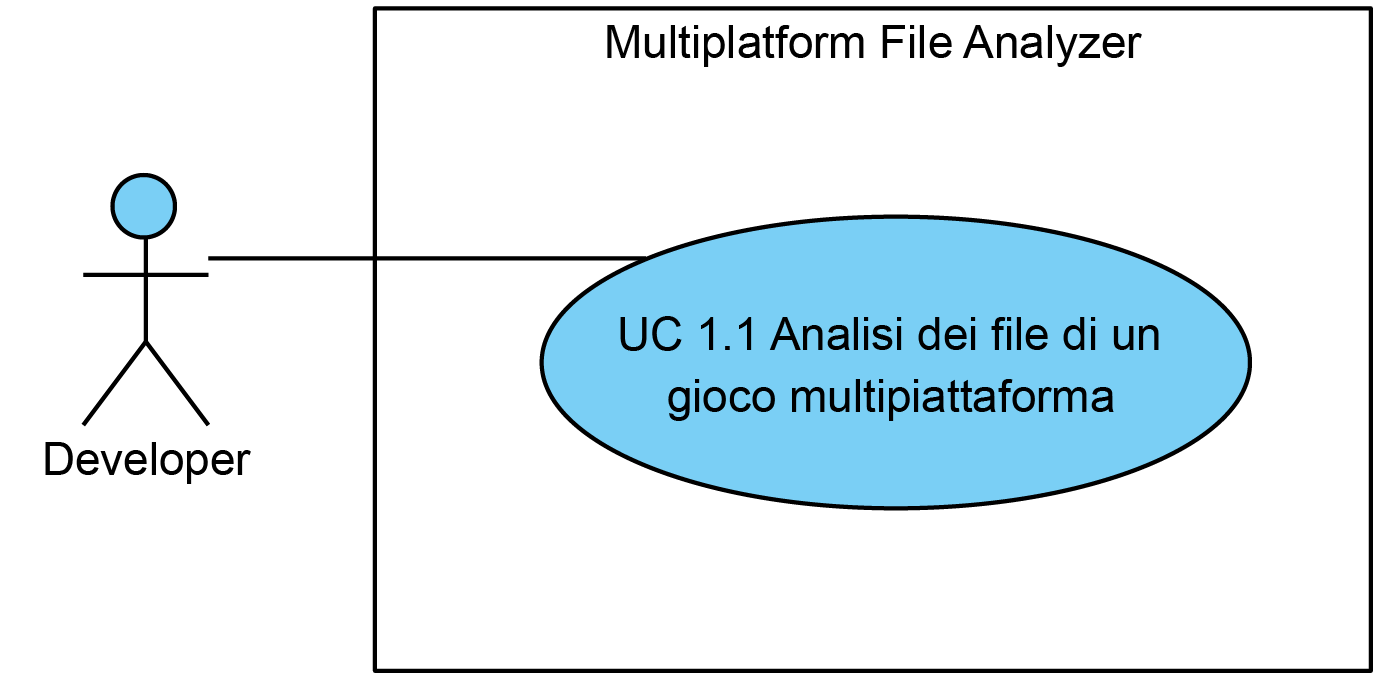
\includegraphics[width=0.9\columnwidth]{tool1/UC1.png} 
			\caption{Use Case - UC 1: Caso d'uso principale}
		\end{figure}
		
		\begin{itemize}
			\item\textbf{Attori}: developer.
			\item\textbf{Descrizione}: un developer può eseguire un'analisi dei file di un gioco multipiattaforma.
			\item\textbf{Precondizione}: il developer abbia lanciato il tool sotto un sistema Windows 7 o superiore.
			\item\textbf{Flusso principale degli eventi}: 
			\begin{enumerate}
				\item\textit{Analisi dei file di un gioco multipiattaforma} (\hyperref[subsec:UC1.1]{UC 1.1}).
			\end{enumerate}
			\item\textbf{Postcondizione}: il sistema ha erogato le funzionalità richieste dal developer.
		\end{itemize}
		
	\subsection{UC 1.1: Analisi dei file di un gioco multipiattaforma}
		\label{subsec:UC1.1}
		
		\begin{figure}[!h] 
			\centering 
			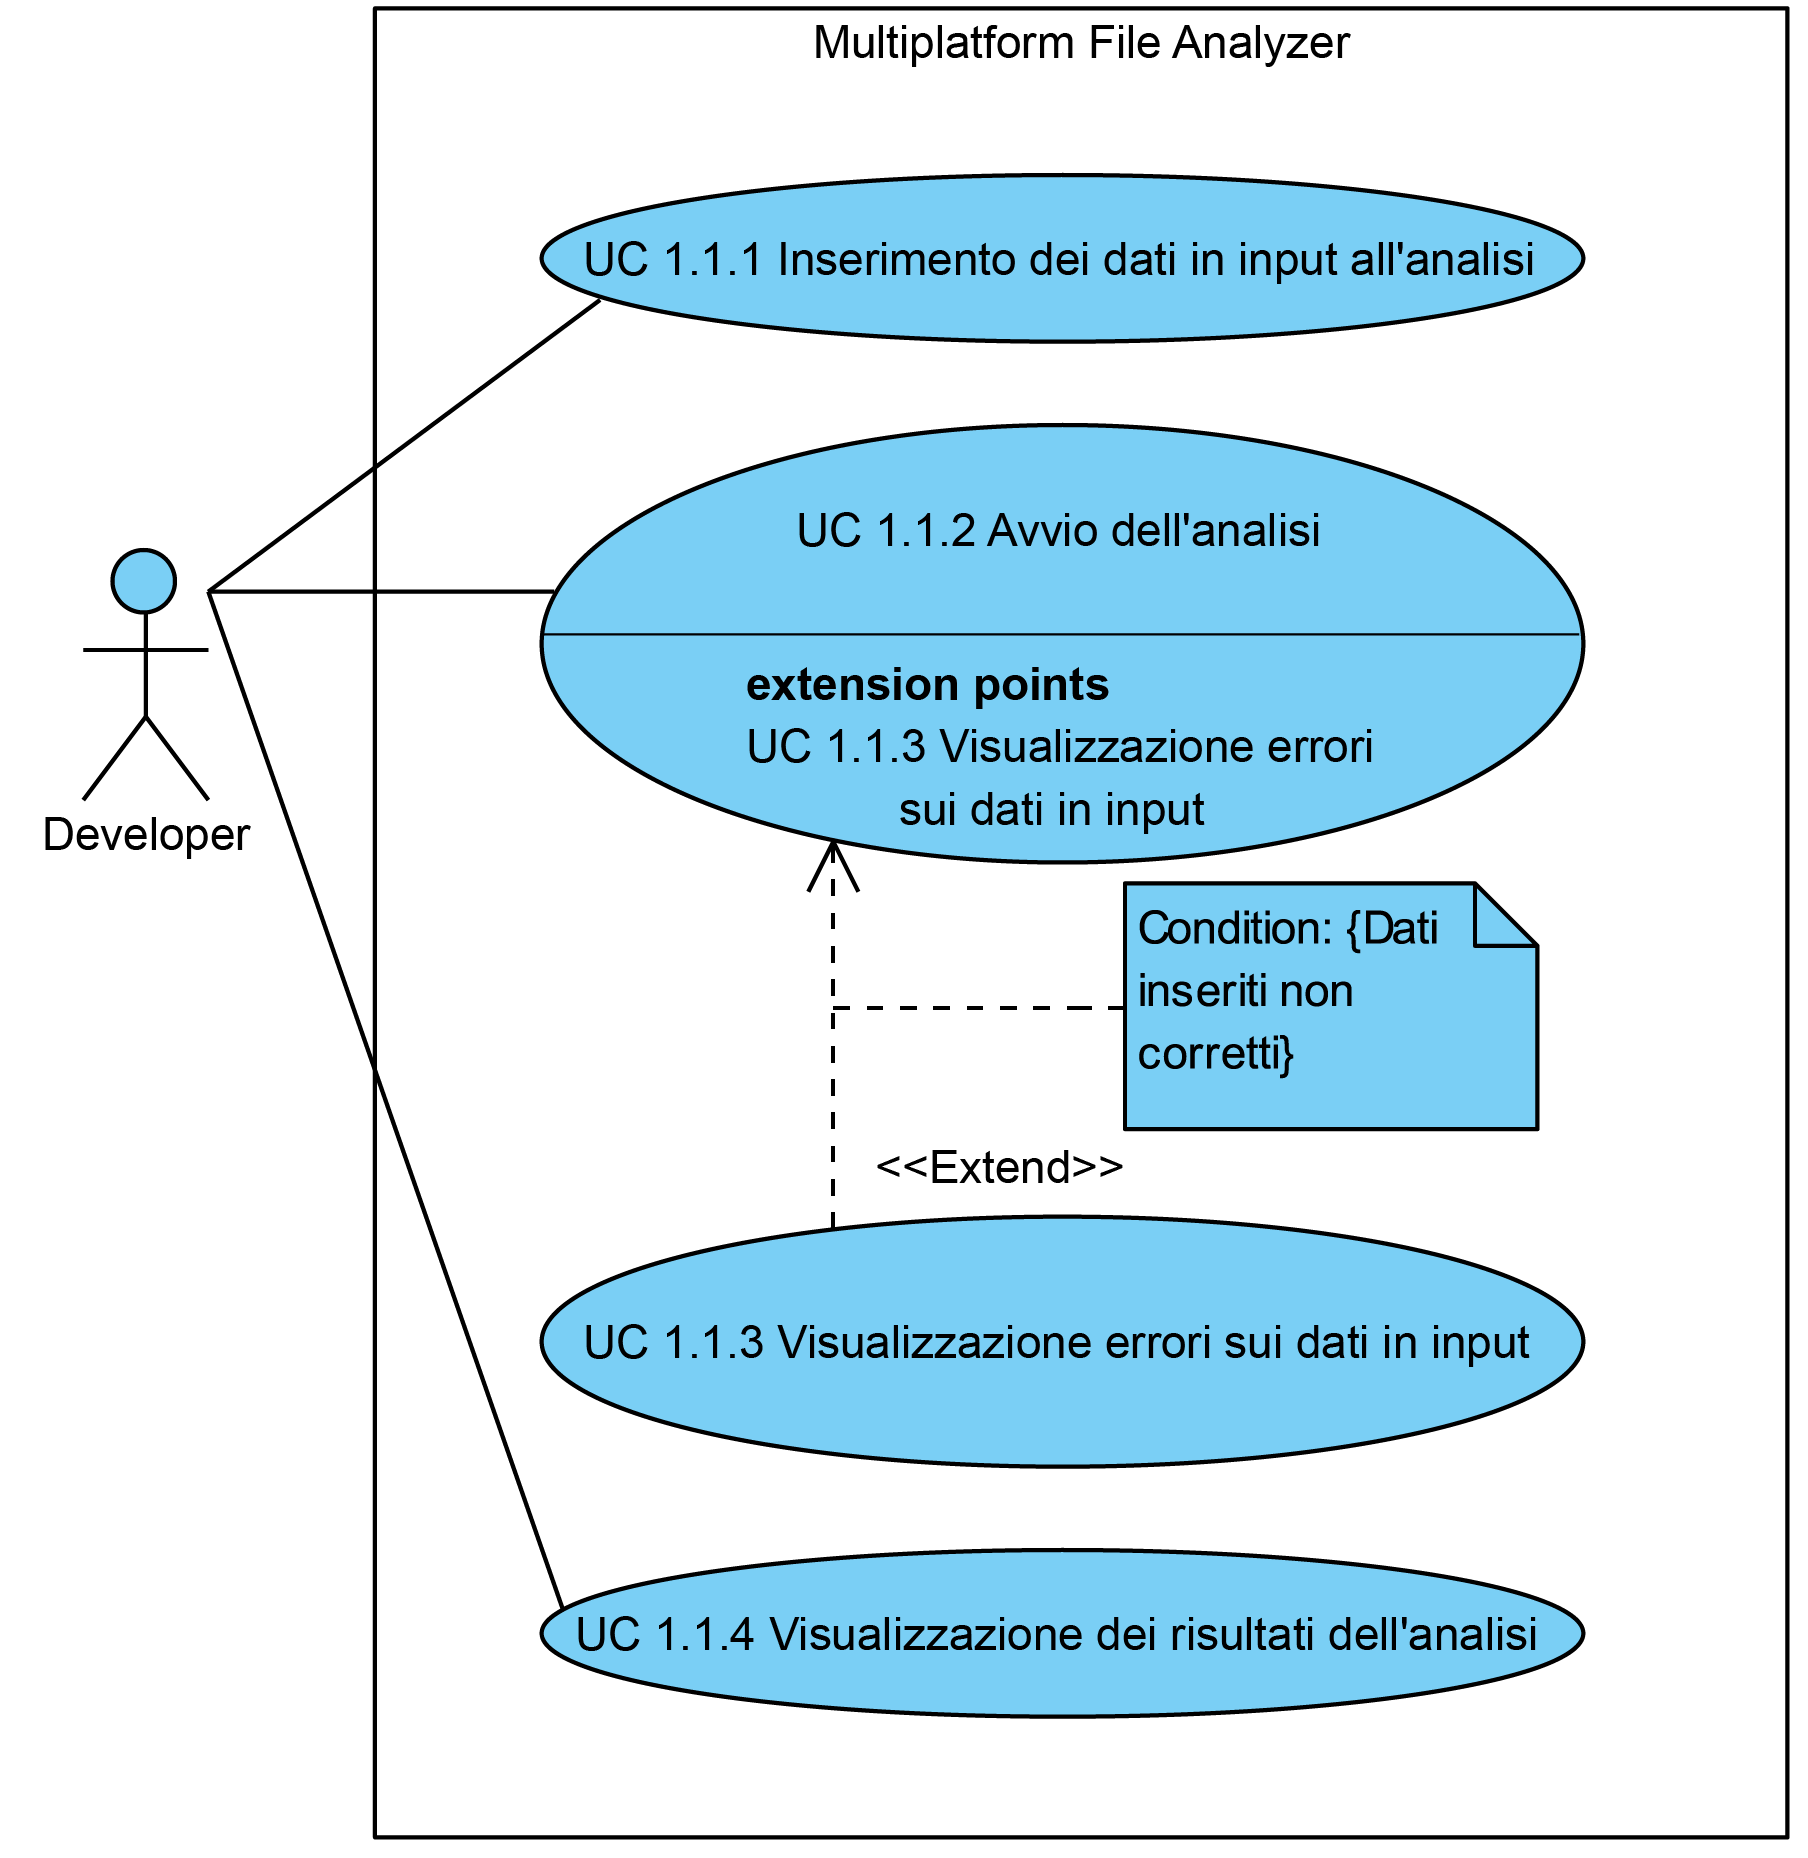
\includegraphics[width=0.9\columnwidth]{tool1/UC1-1.png} 
			\caption{Use Case - UC 1.1: Analisi dei file di un gioco multipiattaforma}
		\end{figure}
		
		\begin{itemize}
			\item\textbf{Attori}: developer.
			\item\textbf{Descrizione}: un developer deve poter inserire i dati necessari all'analisi, visualizzare eventuali errori oppure il risultato dell'analisi.
			\item\textbf{Precondizione}: il developer abbia lanciato il tool sotto un sistema Windows 7 o superiore.
			\item\textbf{Flusso principale degli eventi}: 
			\begin{enumerate}
				\item\textit{Inserimento dei dati in input all'analisi} (\hyperref[subsec:UC1.1.1]{UC 1.1.1});
				\item\textit{Avvio dell'analisi} (\hyperref[subsec:UC1.1.2]{UC 1.1.2});
				\item\textit{Visualizzazione del risultato dell'analisi} (\hyperref[subsec:UC1.1.4]{UC 1.1.4}).
			\end{enumerate}
			\item \textbf{Estensioni}
			\begin{enumerate}
				\item\textit{Visualizzazione errori sui dati in input} (\hyperref[subsec:UC1.1.3]{UC 1.1.3}).
			\end{enumerate}
			\item\textbf{Postcondizione}: il sistema ha erogato le funzionalità richieste dal developer.
		\end{itemize}
	
	\subsection{UC 1.1.1: Inserimento dei dati in input all'analisi}
		\label{subsec:UC1.1.1}
		
		\begin{figure}[!h] 
			\centering 
			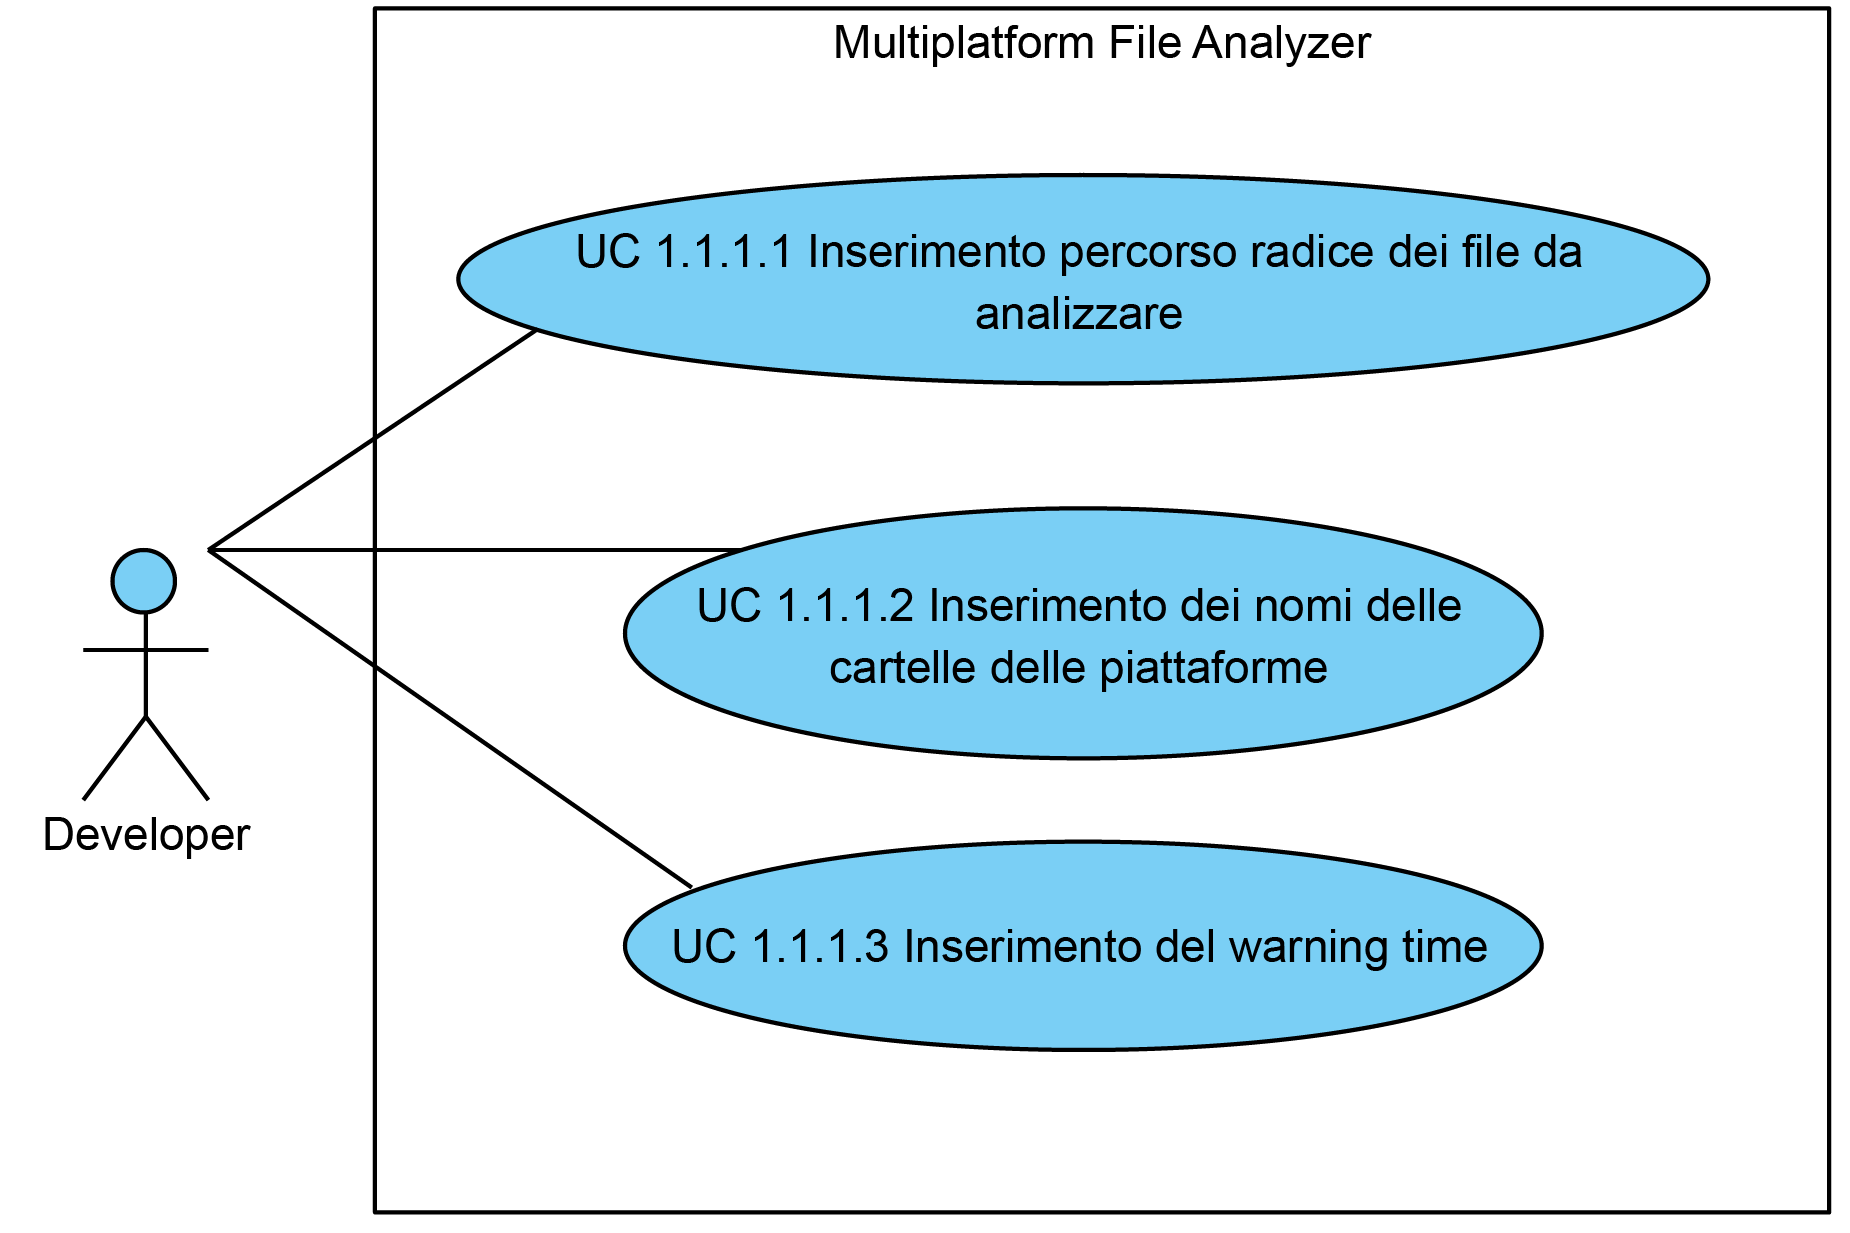
\includegraphics[width=0.9\columnwidth]{tool1/UC1-1-1.png} 
			\caption{Use Case - UC 1.1.1: Inserimento dei dati in input all'analisi}
		\end{figure}
		
		\begin{itemize}
			\item\textbf{Attori}: developer.
			\item\textbf{Descrizione}: un developer deve poter inserire i dati necessari all'analisi composti da un percorso di base, i nomi delle piattaforme e il tempo di warning.
			\item\textbf{Precondizione}: il developer abbia lanciato il tool sotto un sistema Windows 7 o superiore.
			\item\textbf{Flusso principale degli eventi}: 
			\begin{enumerate}
				\item\textit{Inserimento percorso radice dei file da analizzare} (\hyperref[subsec:UC1.1.1.1]{UC 1.1.1.1});
				\item\textit{Inserimento dei nomi delle cartelle delle piattaforme} (\hyperref[subsec:UC1.1.1.2]{UC 1.1.1.2});
				\item\textit{Inserimento del warning time} (\hyperref[subsec:UC1.1.1.3]{UC 1.1.1.3}).
			\end{enumerate}
			\item\textbf{Postcondizione}: il sistema ha preso in carico i dati che verranno usati per la prossima analisi.
		\end{itemize}
		
	\subsection{UC 1.1.1.1: Inserimento percorso radice dei file da analizzare}
		\label{subsec:UC1.1.1.1}
		
		\begin{itemize}
			\item\textbf{Attori}: developer.
			\item\textbf{Descrizione}: il developer deve poter inserire il percorso di base dell'analisi.
			\item\textbf{Precondizione}: il developer abbia lanciato il tool sotto un sistema Windows 7 o superiore.
			\item\textbf{Scenario principale}: il developer sceglie il percorso di base da cui l'analisi partirà.
			\item\textbf{Postcondizione}: il sistema ha preso in carico il percorso di base inserito che verrà usato per la prossima analisi.
		\end{itemize}

	\subsection{UC 1.1.1.2 Inserimento dei nomi delle cartelle delle piattaforme}
		\label{subsec:UC1.1.1.2}
	
		\begin{itemize}
			\item\textbf{Attori}: developer.
			\item\textbf{Descrizione}: il developer deve poter inserire i nomi delle piattaforme da analizzare.
			\item\textbf{Precondizione}: il developer abbia lanciato il tool sotto un sistema Windows 7 o superiore.
			\item\textbf{Scenario principale}: il developer sceglie i nomi delle piattaforme.
			\item\textbf{Postcondizione}: il sistema ha preso in carico i nomi delle piattaforme inserite che verranno usate per la prossima analisi.
		\end{itemize}
		
	\subsection{UC 1.1.1.3 Inserimento del warning time}
		\label{subsec:UC1.1.1.3}
		
		\begin{itemize}
			\item\textbf{Attori}: developer.
			\item\textbf{Descrizione}: il developer deve poter inserire il tempo di warning.
			\item\textbf{Precondizione}: il developer abbia lanciato il tool sotto un sistema Windows 7 o superiore.
			\item\textbf{Scenario principale}: il developer il tempo superato il quale vuole essere avvertito.
			\item\textbf{Postcondizione}: il sistema ha preso in carico il tempo di warning che verrà usato per la prossima analisi.
		\end{itemize}
		
	\subsection{UC 1.1.2 Avvio dell'analisi}
		\label{subsec:UC1.1.2}
		
		\begin{itemize}
			\item\textbf{Attori}: developer.
			\item\textbf{Descrizione}: il developer deve poter avviare la ricerca.
			\item\textbf{Precondizione}: il developer abbia lanciato il tool sotto un sistema Windows 7 o superiore.
			\item\textbf{Scenario principale}: il developer sceglie di avviare la ricerca.
			\item\textbf{Postcondizione}: il sistema inizia a eseguire l'analisi.
		\end{itemize}

	\subsection{UC 1.1.3 Visualizzazione errori sui dati in input}
		\label{subsec:UC1.1.3}
	
		\begin{itemize}
			\item\textbf{Descrizione}: il developer ha commesso uno dei seguenti errori durante l'inserimento dei dati in input all'analisi:
			\begin{itemize}
				\item il percorso inserito non è valido;
				\item il developer non ha inserito nessuna piattaforma.
			\end{itemize}
			\item\textbf{Precondizione}: il developer abbia avviato la ricerca.
			\item\textbf{Scenario principale}: viene fornita una spiegazione dell'errore commesso e come risolverlo.
			\item\textbf{Postcondizione}: l'errore commesso è stato visualizzato e spiegato, l'analisi non è stata avviata.
		\end{itemize}

	\subsection{UC 1.1.4 Visualizzazione dei risultati dell'analisi}
		\label{subsec:UC1.1.4}
		
		\begin{figure}[!h] 
			\centering 
			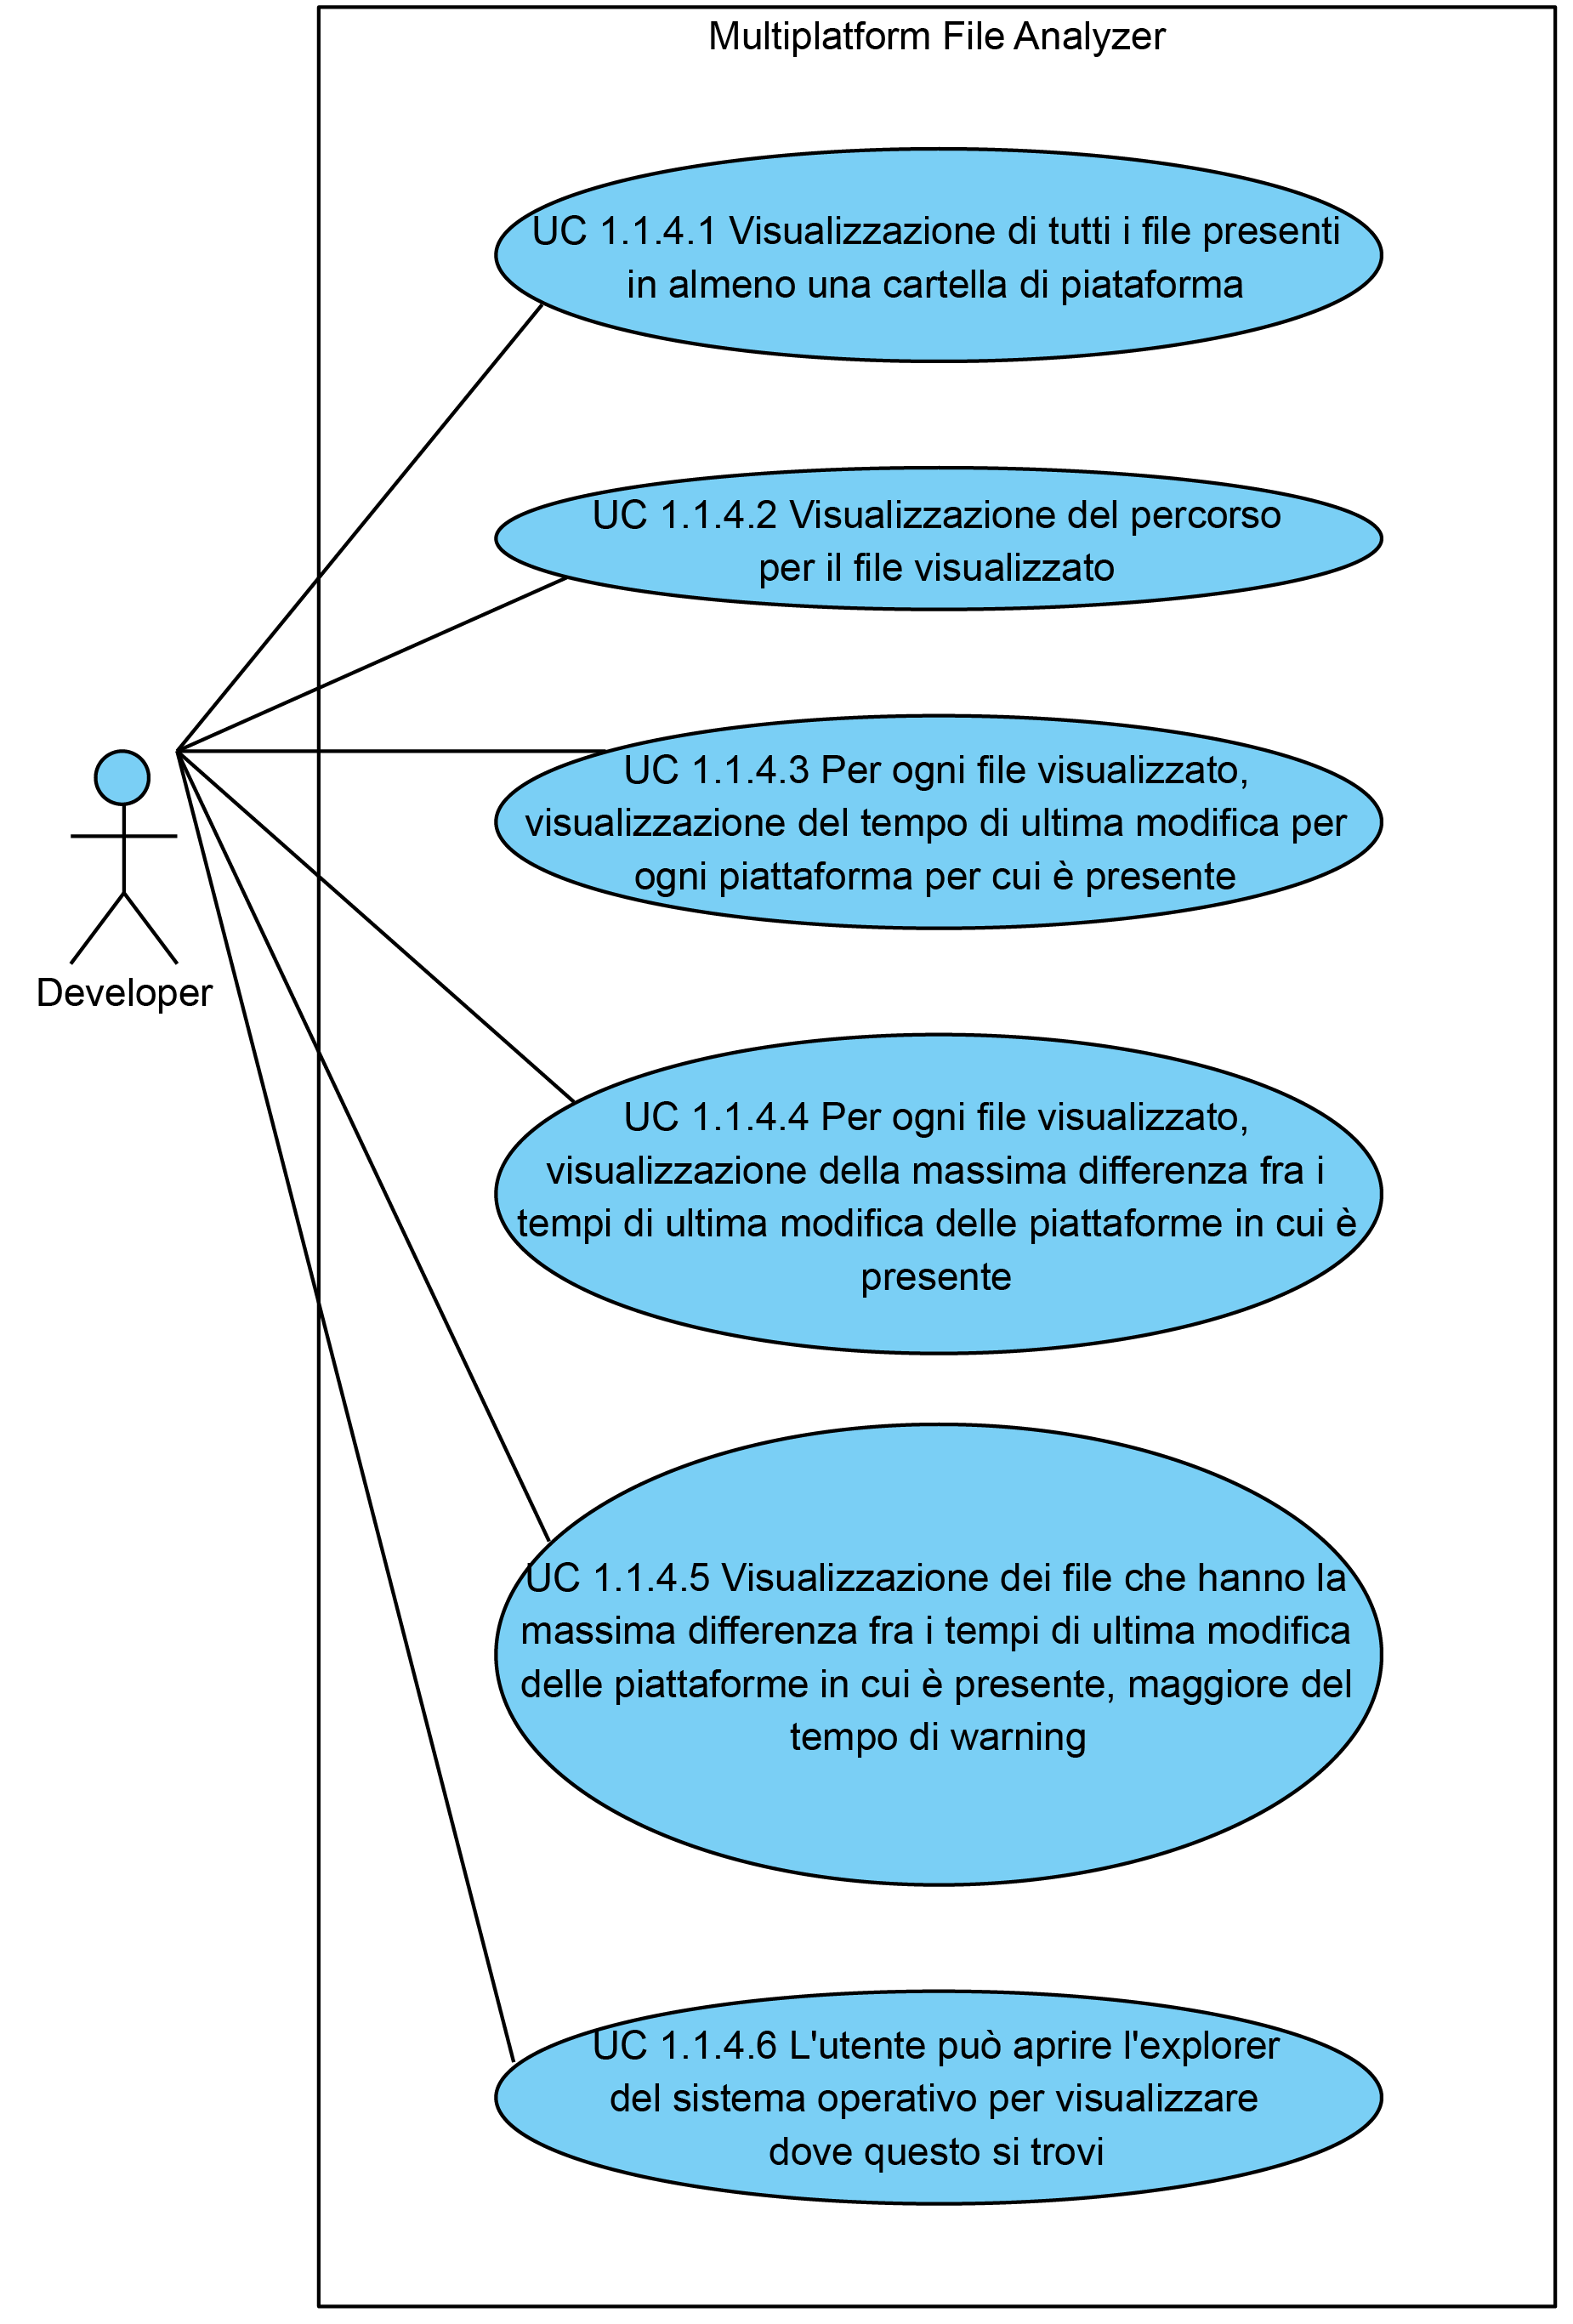
\includegraphics[width=0.9\columnwidth]{tool1/UC1-1-4.png} 
			\caption{Use Case - UC 1.1.4: Visualizzazione dei risultati dell'analisi}
		\end{figure}
		
		\begin{itemize}
			\item\textbf{Attori}: developer.
			\item\textbf{Descrizione}: un developer deve poter inserire i dati necessari all'analisi composti da un percorso di base, i nomi delle piattaforme e il tempo di warning.
			\item\textbf{Precondizione}: il developer abbia avviato l'analisi e che questa abbia terminato senza comunicare nessun errore sui dati in input.
			\item\textbf{Flusso principale degli eventi}: 
			\begin{enumerate}
				\item\textit{Visualizzazione di tutti i file presenti in almeno una cartella di piattaforma} (\hyperref[subsec:UC1.1.4.1]{UC 1.1.4.1});
				
				\item\textit{Visualizzazione del percorso per il file visualizzato} (\hyperref[subsec:UC1.1.4.2]{UC 1.1.4.2});
				
				\item\textit{Per ogni file visualizzato, visualizzazione del tempo di ultima modifica per ogni piattaforma per cui è presente} (\hyperref[subsec:UC1.1.4.3]{UC 1.1.4.3});
				
				\item\textit{Per ogni file visualizzato, visualizzazione della massima differenza fra i tempi di ultima modifica delle piattaforme in cui è presente} (\hyperref[subsec:UC1.1.4.4]{UC 1.1.4.4});
				
				\item\textit{Visualizzazione dei file che hanno la massima differenza fra i tempi di ultima modifica delle piattaforme in cui è presente, maggiore del tempo di warning} (\hyperref[subsec:UC1.1.4.5]{UC 1.1.4.5});
				
				\item\textit{Il developer può aprire l'explorer del sistema operativo per visualizzare dove questo si trovi} (\hyperref[subsec:UC1.1.4.6]{UC 1.1.4.6});
				
			\end{enumerate}
			\item\textbf{Postcondizione}: i dati dell'analisi sono stati visualizzati.
		\end{itemize}

	\subsection{UC 1.1.4.1 Visualizzazione di tutti i file presenti in almeno una cartella di piattaforma}
		\label{subsec:UC1.1.4.1}
		
		\begin{itemize}
			\item\textbf{Attori}: developer.
			\item\textbf{Descrizione}: il developer deve poter visualizzare tutti i file che sono stati trovati in almeno una piattaforma.
			\item\textbf{Precondizione}: il developer abbia avviato l'analisi e che questa abbia terminato senza comunicare nessun errore sui dati in input.
			\item\textbf{Scenario principale}: vengono visualizzati i file presenti in almeno una piattaforma.
			\item\textbf{Postcondizione}: il risultato dell'analisi è stato visualizzato.
		\end{itemize}
	
	\subsection{UC 1.1.4.2 Visualizzazione del percorso per il file visualizzato}
		\label{subsec:UC1.1.4.2}
	
		\begin{itemize}
			\item\textbf{Attori}: developer.
			\item\textbf{Descrizione}: il developer deve poter visualizzare il percorso del file visualizzato.
			\item\textbf{Precondizione}: il developer abbia avviato l'analisi e che questa abbia terminato senza comunicare nessun errore sui dati in input.
			\item\textbf{Scenario principale}: il developer visualizza il percorso del file visualizzato.
			\item\textbf{Postcondizione}: il percorso del file è stato visualizzato.
		\end{itemize}

	\subsection{UC 1.1.4.3 Per ogni file visualizzato, visualizzazione del tempo di ultima modifica per ogni piattaforma per cui è presente}
		\label{subsec:UC1.1.4.3}
		
		\begin{itemize}
			\item\textbf{Attori}: developer.
			\item\textbf{Descrizione}: il developer deve poter visualizzare il tempo di ultima modifica per ciascuna piattaforma in cui il file è stato trovato.
			\item\textbf{Precondizione}: il developer abbia avviato l'analisi e che questa abbia terminato senza comunicare nessun errore sui dati in input.
			\item\textbf{Scenario principale}: viene visualizzata la data di ultima modifica per ciascuna piattaforma.
			\item\textbf{Postcondizione}: il risultato dell'analisi è stato visualizzato.
		\end{itemize}
		
	\subsection{UC 1.1.4.4 Per ogni file visualizzato, visualizzazione della massima differenza fra i tempi di ultima modifica delle piattaforme in cui è presente}
		\label{subsec:UC1.1.4.4}
	
		\begin{itemize}
			\item\textbf{Attori}: developer.
			\item\textbf{Descrizione}: il developer deve poter visualizzare la massima differenza fra i tempi di ultima modifica delle piattaforme in cui è presente il file.
			\item\textbf{Precondizione}: il developer abbia avviato l'analisi e che questa abbia terminato senza comunicare nessun errore sui dati in input.
			\item\textbf{Scenario principale}: viene visualizzata la massima differenza fra i tempi di ultima modifica.
			\item\textbf{Postcondizione}: la massima differenza fra i tempi di ultima modifica è stata visualizzata.
		\end{itemize}
		
	\subsection{UC 1.1.4.5 Visualizzazione dei file che hanno la massima differenza fra i tempi di ultima modifica delle piattaforme in cui è presente, maggiore del tempo di warning}
		\label{subsec:UC1.1.4.5}
	
		\begin{itemize}
			\item\textbf{Attori}: developer.
			\item\textbf{Descrizione}: il developer deve poter visualizzare e riconoscere i file per i quali la massima differenza fra i tempi di ultima modifica è maggiore del tempo di warning.
			\item\textbf{Precondizione}: il developer abbia avviato l'analisi e che questa abbia terminato senza comunicare nessun errore sui dati in input.
			\item\textbf{Scenario principale}: vengono visualizzati tutti i file che superano il tempo di warning.
			\item\textbf{Postcondizione}: i file che superano il tempo di warning sono stati visualizzati.
		\end{itemize}
			
	\subsection{UC 1.1.4.6 L'utente può aprire l'explorer del sistema operativo per visualizzare dove questo si trovi}
		\label{subsec:UC1.1.4.6}
	
		\begin{itemize}
			\item\textbf{Attori}: developer.
			\item\textbf{Descrizione}: il developer deve poter aprire il programma che permettere l'esplorazione del file system nel punto in cui è presente il file correntemente selezionato.
			\item\textbf{Precondizione}: il developer abbia avviato l'analisi e che questa abbia terminato senza comunicare nessun errore sui dati in input.
			\item\textbf{Scenario principale}: viene visualizzato il file nella sua posizione all'interno del file system.
			\item\textbf{Postcondizione}: il file viene visualizzato nella sua posizione all'interno del file system.
		\end{itemize}


\section{Tracciamento dei requisiti}

	Partendo dai casi d'uso si è provveduto a stilare una precisa analisi dei requisiti per il tool in questione. I requisiti trovati sono stati inoltre tracciati in relazione al caso d'uso di origine.\\

	Di seguito vengono riportati tutti i requisiti individuati. Per essere più leggibili verranno separati in tabelle a seconda della loro categoria. Di ogni requisito verranno indicati: tipologia, importanza e provenienza.\\
	I requisiti dovranno essere classificati per tipo e importanza e utilizzeranno la seguente sintassi:
	\begin{center}
		R[Importanza][Tipo][Codice]
	\end{center}
	\begin{itemize}
		\item \textbf{Importanza}: può assumere solo uno fra i seguenti valori:
		\begin{itemize}
			\item \textit{0}: requisito obbligatorio;
			\item \textit{1}: requisito desiderabile;
			\item \textit{2}: requisito opzionale.
		\end{itemize}
		\item \textbf{Tipo}: pu\`{o} assumere solo uno fra i seguenti valori:
		\begin{itemize}
			\item  \textit{F}: funzionale;
			\item  \textit{Q}: di qualità;
			\item  \textit{P}: prestazionale;
			\item  \textit{V}: vincolo.
		\end{itemize}
		\item \textbf{Codice}: è il codice gerarchico univoco di ogni vincolo espresso in numeri (esempio: 1.3.2).
	\end{itemize}
	
	Per ogni requisito vengono inoltre specificati:
	\begin{itemize}
		\item \textbf{descrizione}: breve ma completa ed il \underline{meno} ambigua possibile;
		\item \textbf{fonte}: pu\`{o} essere soltanto una o pi\`{u} tra le seguenti:
		\begin{itemize}
			\item \textit{caso d'uso}: il requisito \`{e} stato estrapolato da un caso d'uso. In questo caso va indicato il codice univoco del caso d'uso. \`{E} possibile indicare come fonte pi\`{u} di un caso d'uso.
			\item \textit{interno}: è stato ritenuto giusto aggiungere questo requisito per completezza.
			\item \textit{tutor aziendale}: il requisito è stato espressamente richiesto dal tutor aziendale.
		\end{itemize}
	\end{itemize}
	
	\subsection{Requisiti funzionali}
		\begin{center}
			\begin{longtable}{p{4.2cm}!{\color{white}\vrule width 0.5mm}p{6cm}!{\color{white}\vrule width 0.5mm}p{2.5cm}!{\color{white}\vrule width 0.5mm}}
				\rowcolor{headcolor}\textcolor{white}{\textbf{Requisito}}&\textcolor{white}{\textbf{Descrizione}}&\textcolor{white}{\textbf{Fonti}}\\
				
				\rowcolor{row1}\hspace{0mm}\hypertarget{R0F1}{R0F1}  & Un utente può effettuare l'analisi dei file di un gioco multipiattaforma. & \hyperref[subsec:UC1.1]{UC 1.1}\\
				
				
				\rowcolor{row2}\hspace{2mm}\hypertarget{R0F1.1}{R0F1.1}  & L'analisi richiede l'inserimento di dati in input. & \hyperref[subsec:UC1.1.1]{UC 1.1.1}\\
				
				\rowcolor{row1}\hspace{4mm}\hypertarget{R0F1.1.1}{R0F1.1.1}  & L'analisi richiede l'inserimento di un percorso assoluto dal quale far partire l'analisi. & \hyperref[subsec:UC1.1.1.1]{UC 1.1.1.1}\\
				
				\rowcolor{row2}\hspace{4mm}\hypertarget{R0F1.1.2}{R0F1.1.2}  & L'analisi richiede l'inserimento dei nomi delle cartelle identificative di file di piattaforma. & \hyperref[subsec:UC1.1.1.2]{UC 1.1.1.2}\\
				
				\rowcolor{row1}\hspace{6mm}\hypertarget{R0F1.1.2.1}{R0F1.1.2.1}  & Il programma interpreta i nomi delle piattaforme in modo "case-insensitive". & \hyperref[subsec:UC1.1.1.2]{UC 1.1.1.2}\\
				
				\rowcolor{row2}\hspace{6mm}\hypertarget{R0F1.1.2.2}{R0F1.1.2.2}  & Il programma richiede l'inserimento dei nomi delle piattaforme come unica stringa utilizzando il carattere \sq{;} come separatore. & \hyperref[subsec:UC1.1.1.2]{UC 1.1.1.2}\\
				
				\rowcolor{row1}\hspace{4mm}\hypertarget{R0F1.1.3}{R0F1.1.3}  & L'analisi richiede l'inserimento di un tempo di warning, superato il quale, a fine l'analisi, verrà segnalato il problema se presente. & \hyperref[subsec:UC1.1.1.3]{UC 1.1.1.3}\\
				
				\rowcolor{row2}\hspace{6mm}\hypertarget{R0F1.1.3.1}{R0F1.1.3.1}  & Il formato del tempo di warning accettato prevede l'utilizzo esclusivo di numeri in formato inglese e con massimo due cifre decimali. & \hyperref[subsec:UC1.1.1.3]{UC 1.1.1.3}\\
				
				
				\rowcolor{row1}\hspace{4mm}\hypertarget{R0F1.1.4}{R0F1.1.4}  & Il programma deve memorizzare e pre inserire i dati della precedente analisi (se esistenti) negli appositi campi per l'input dei dati, anche se tra un'analisi e la successiva il programma è stato chiuso. & Interno\\
				
				
				\rowcolor{row2}\hspace{2mm}\hypertarget{R0F1.3}{R0F1.3} & Il programma mostra gli eventuali errori sui dati in input all'analisi trovati durante l'avvio della stessa. & \hyperref[subsec:UC1.1.3]{UC 1.1.3}\\
				
				\rowcolor{row1}\hspace{4mm}\hypertarget{R0F1.3.1}{R0F1.3.1} & Il programma ferma l'avvio dell'analisi se il percorso di base non viene fornito. & \hyperref[subsec:UC1.1.3]{UC 1.1.3}\\
				
				\rowcolor{row2}\hspace{4mm}\hypertarget{R0F1.3.2}{R0F1.3.2} & Il programma ferma l'avvio dell'analisi se il percorso di base inserito non è un percorso assoluto. & \hyperref[subsec:UC1.1.3]{UC 1.1.3}\\
				
				\rowcolor{row1}\hspace{4mm}\hypertarget{R0F1.3.3}{R0F1.3.3} & Il programma ferma l'avvio dell'analisi se il percorso di base inserito non esiste nel file system. & \hyperref[subsec:UC1.1.3]{UC 1.1.3}\\
				
				\rowcolor{row2}\hspace{4mm}\hypertarget{R0F1.3.4}{R0F1.3.4} & Il programma ferma l'avvio dell'analisi se il contenuto del percorso di base inserito non è leggibile. & \hyperref[subsec:UC1.1.3]{UC 1.1.3}\\
				
				
				\rowcolor{row1}\hspace{2mm}\hypertarget{R0F1.4}{R0F1.4} & Il programma permette la visualizzazione dei dati output dell'analisi. & \hyperref[subsec:UC1.1.4]{UC 1.1.4}\\
				
				\rowcolor{row2}\hspace{4mm}\hypertarget{R0F1.4.1}{R0F1.4.1} & Nell'output dell'analisi è presente ciascun file presente in almeno un cartella di piattaforma. & \hyperref[subsec:UC1.1.4.1]{UC 1.1.4.1}\\
				
				\rowcolor{row1}\hspace{4mm}\hypertarget{R0F1.4.2}{R0F1.4.2} & Per ciascun file presente nell'output è visibile la data di ultima modifica per ciascuna piattaforma in cui è presente. & \hyperref[subsec:UC1.1.4.2]{UC 1.1.4.2}\\
				
				\rowcolor{row2}\hspace{4mm}\hypertarget{R0F1.4.3}{R0F1.4.3} & Per ciascun file presente nell'output è indicato il percorso di relativo a partire dal percorso di base inserito in input all'analisi. & \hyperref[subsec:UC1.1.4.3]{UC 1.1.4.3}\\
				
				\rowcolor{row1}\hspace{4mm}\hypertarget{R0F1.4.4}{R0F1.4.4} & Per ciascun file presente nell'output è indicato il nome del file completo di estensione. & \hyperref[subsec:UC1.1.4.4]{UC 1.1.4.4}\\
				
				\rowcolor{row2}\hspace{4mm}\hypertarget{R0F1.4.5}{R0F1.4.5} & Per ciascun file presente nell'output è indicata la massima differenza tra le date di ultima modifica delle piattaforme per cui è presente & \hyperref[subsec:UC1.1.4.5]{UC 1.1.4.5}\\
				
				\rowcolor{row1}\hspace{6mm}\hypertarget{R0F1.4.5.1}{R0F1.4.5.1} & Se il tempo massimo per ciascuno file è superiore al tempo di warning inserito in input allora questo viene evidenziato come warning. & \hyperref[subsec:UC1.1.4.5]{UC 1.1.4.5}\\
				
				\rowcolor{row2}\hspace{6mm}\hypertarget{R0F1.4.5.2}{R0F1.4.5.2} & Il tempo è mostrato nella stessa unità di misura in cui è stato inserito il tempo di warning. & \hyperref[subsec:UC1.1.4.5]{UC 1.1.4.5}\\
				
				\rowcolor{row1}\hspace{4mm}\hypertarget{R0F1.4.6}{R0F1.4.6} & Il programma permette di aprire il programma per esplorare il file system di default del sistema e visualizzare la cartella dove è presente il file & \hyperref[subsec:UC1.1.4.6]{UC 1.1.4.6}\\
				
				\hline
				\caption{Requisiti funzionali}
			\end{longtable}
		\end{center}

	\subsection{Requisiti di qualità}
		\begin{center}
			\begin{longtable}{p{4.2cm}!{\color{white}\vrule width 0.5mm}p{6cm}!{\color{white}\vrule width 0.5mm}p{2.5cm}!{\color{white}\vrule width 0.5mm}}
				\rowcolor{headcolor}\textcolor{white}{\textbf{Requisito}}&\textcolor{white}{\textbf{Descrizione}}&\textcolor{white}{\textbf{Fonti}}\\
				
				\rowcolor{row1}\hspace{0mm}\hypertarget{R0Q1}{R0Q1} & Viene fornito insieme al programma un l'help con la guida alla compilazione e al deploy per sistemi Windows. & Tutor interno\\
				
				\rowcolor{row2}\hspace{0mm}\hypertarget{R0Q2}{R0Q2} & Viene fornito un l'help che spiega come utilizzare il programma. & Tutor interno\\
				
				\hline
				\caption{Requisiti di vincolo}
			\end{longtable}
		\end{center}

	\subsection{Requisiti di vincolo}
		\begin{center}
			\begin{longtable}{p{4.2cm}!{\color{white}\vrule width 0.5mm}p{6cm}!{\color{white}\vrule width 0.5mm}p{2.5cm}!{\color{white}\vrule width 0.5mm}}
				\rowcolor{headcolor}\textcolor{white}{\textbf{Requisito}}&\textcolor{white}{\textbf{Descrizione}}&\textcolor{white}{\textbf{Fonti}}\\
				
				\rowcolor{row1}\hspace{0mm}\hypertarget{R0V1}{R0V1} & Il programma deve funzionare su Windows 7 SP1 32 e 64 bit. & Tutor interno\\
				
				\rowcolor{row2}\hspace{0mm}\hypertarget{R0V2}{R0V2} & Il programma deve essere scritto utilizzando il linguaggio C++ 98. & Tutor interno\\
				
				\hline
				\caption{Requisiti di vincolo}
			\end{longtable}
		\end{center}
		
\section{Tecnologie e strumenti}
	Di seguito viene fornita una panoramica delle tecnologie e strumenti utilizzati per lo sviluppo di Multiplatform File Analyzer.
	
	\subsection{Qt\textsuperscript{\textregistered} Framework}
		Per lo sviluppo del tool è stato usato Qt\textsuperscript{\textregistered} Framework versione 5.3.1. Qt\textsuperscript{\textregistered} è un potente Framework multipiattaforma che offre una vastissima serie di librerie di utilità, grazie alle quali lo sviluppo diviene agevole e veloce, permettendo quasi  sempre di non legarsi a specifiche implementazioni per piattaforma.\\
		In particolare è stata usata la libreria per costruire le interfacce grafiche e la libreria per accedere al file system e leggerne le informazioni.
		
	\subsection{Qt\textsuperscript{\textregistered} Creator}
		Come IDE per lo sviluppo ci si è affidati a Qt\textsuperscript{\textregistered} Creator 3.1.2. IDE semplice e performante che si integra perfettamente con il mondo Qt\textsuperscript{\textregistered}, offrendo addirittura la consultazione veloce della documentazione direttamente nell'IDE.
		
\section{Ciclo di vita del software}
	Essendo Multiplatform File Analyzer uno strumento di piccole dimensioni si è adottato un semplice modello di ciclo di vita incrementale, con un singolo incremento corrispondente alla consegna finale.
	
\section{Progettazione}
	Il software è stato progettato per offrire una semplice espandibilità, allo scopo la strutturazione generale segue il collaudato Design Pattern \textit{MVC}, dove trovano luogo i seguenti pacchetti: \texttt{controller}, \texttt{view} e \texttt{data}. È inoltre presente il pacchetto \texttt{core} in cui è inserita l'implementazione degli algoritmi di business del tool, ad esempio l'algoritmo che esegue l'analisi.\\
	
	Il pacchetto \texttt{core} è implementato con il Design Pattern \textit{Strategy} allo scopo di permettere una facile estensione o sostituzione dell'algoritmo che esegue l'analisi, anche a run-time.\\
	
	Per permettere una facile e veloce connessione tra gli strati descritti dall'\textit{MVC} è stato adottato il Design Pattern \textit{Observer}, implementato nell'omonimo pacchetto \textit{observer}.\\
	
	È stato scelto di utilizzare il Design Pattern \textit{Strategy} per rendere modificabile facilmente l'implementazione dell'algoritmo che effettua l'analisi, all'interno del pacchetto \texttt{core}.\\
	
	È stato inoltre cercato di utilizzare le classi del Framework Qt\textsuperscript{\textregistered} in modo isolato alle sole parti strettamente necessarie, ovvero la GUI e l'analisi del file system. Questo allo scopo di rendere il tool slegato dalle implementazioni specifiche, in favore di una più semplice espandibilità.
	
	\subsection{Diagramma delle classi}
		Di seguito è presente il diagramma delle classi espresso tramite il formalismo UML 2.0. Nel diagramma è inoltre possibile vedere le principali dipendenza verso le classi del Framework Qt\textsuperscript{\textregistered}.
		
		\begin{figure}[!h] 
			\centering 
			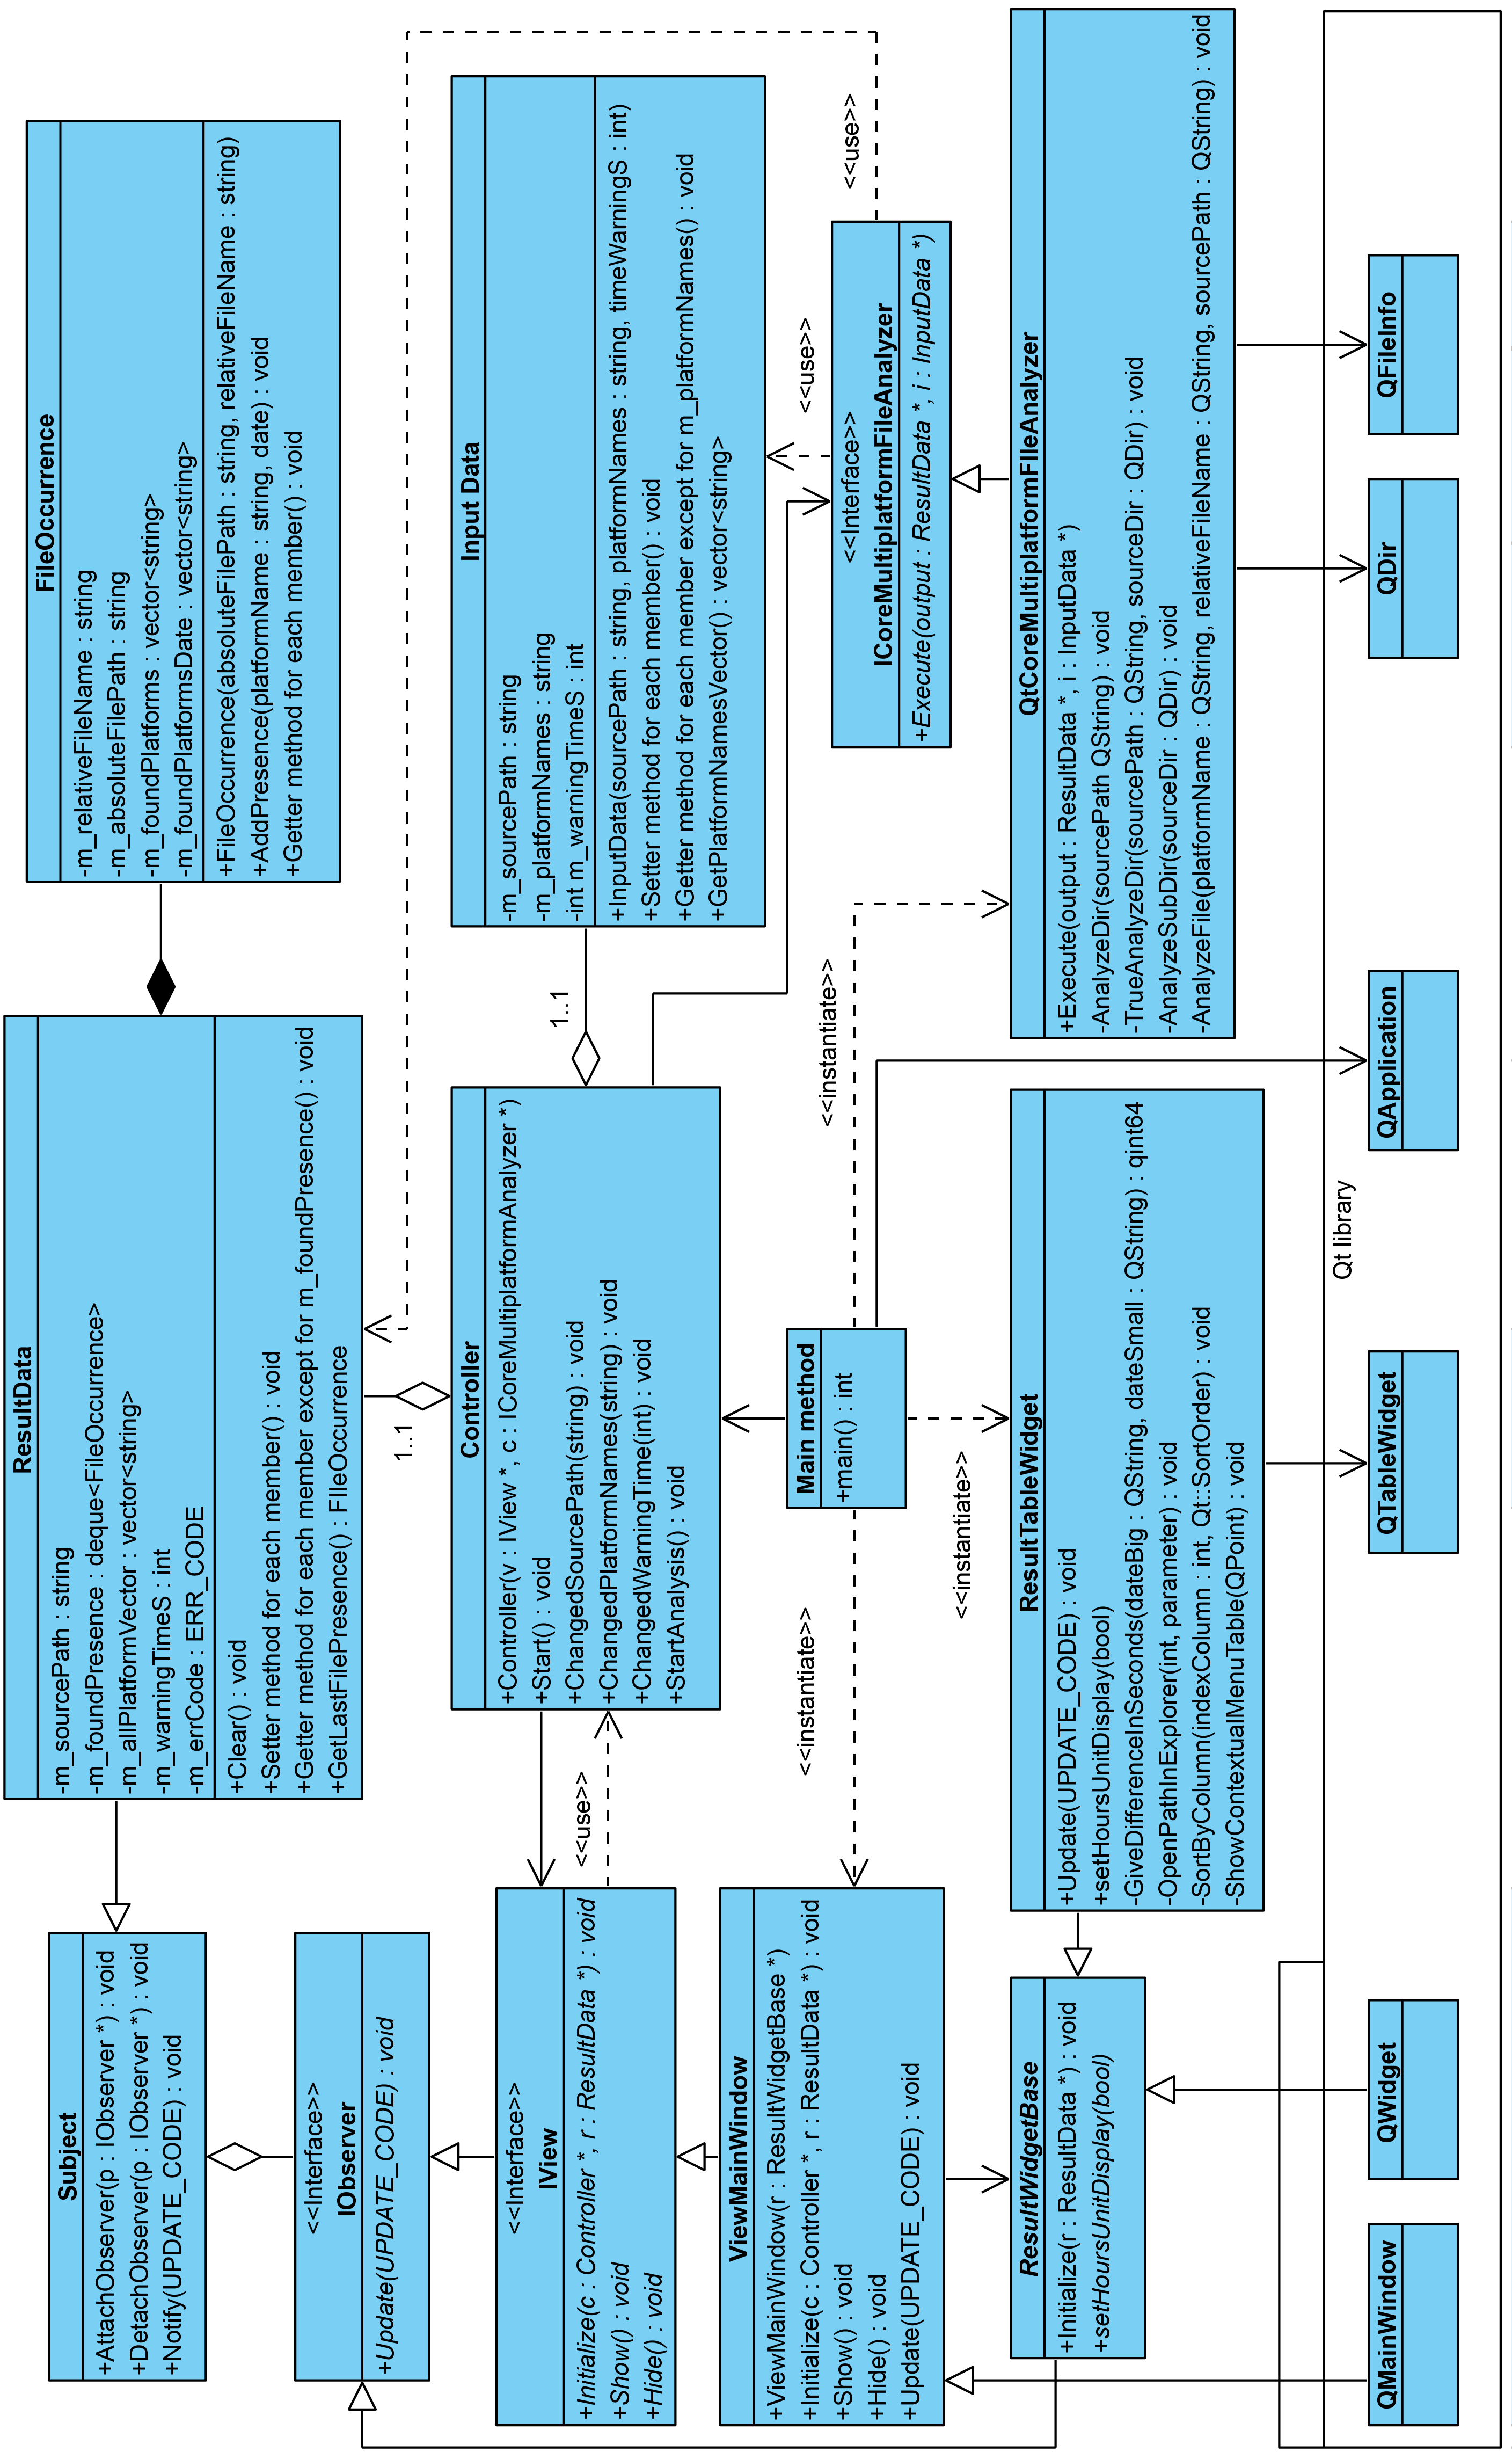
\includegraphics[width=0.98\columnwidth]{tool1/Tool-1-Diagramma-Classi.png} 
			\caption{Diagramma delle classi di Multiplatform File Analyzer}
		\end{figure}
	
		\newpage
	
	\subsection{Pacchetto controller}
		Il pacchetto è composto dalla sola classe \texttt{Controller} che svolge il compito di controllore del sistema. È questo il solo pacchetto utilizzato dalla funzione \texttt{main}.
		
		\subsubsection{Classe Controller}
			La classe \texttt{Controller} si occupa di avviare il sistema. Essa provvede ad allocare tutti gli oggetti necessari e al relativo rilascio al termine del programma. Inoltre seleziona la view e la connette con le classi che rappresentano i dati. Infine raccoglie i comandi utente provenienti dalla view e li esegue grazie al pacchetto \texttt{core}.
	
	\subsection{Pacchetto observer}
		Questo pacchetto rappresenta l'implementazione del Design Pattern \textit{Observer} ed è stato utilizzato per tenere aggiornata la view al cambiamento dei dati.
		
		\subsubsection{Interfaccia IObserver}
		\texttt{IObserver} è l'interfaccia che rappresenta gli oggetti che osservano le modifiche di altri oggetti. Essa contiene il metodo virtuale puro \texttt{Update} che i soggetti osservati invocano per segnalare il fatto che sono stati modificati e che quindi un aggiornamento è necessario. Le classi concrete che avranno la necessità di osservare un soggetto deriveranno da \texttt{IObserver} implementando il metodo \texttt{Update}.
		
		\subsubsection{Classe Subject}
		La classe \texttt{Subject} rappresenta un soggetto che può essere osservato. Essa contiene il codice necessario per notificare tutti gli osservatori dell'avvenuto cambiamento. Mantiene inoltre una lista degli osservatori da notificare, i quali possono iscriversi se desiderano ricevere la notifica, oppure rimuoversi se non è più necessario ricevere aggiornamenti. Le classi che devono essere osservate deriveranno da questa.
	
	\subsection{Pacchetto data}
		Il pacchetto \texttt{data} contiene tutte le classi che rappresentano i dati di business del programma. Allo scopo di rendere il programma eseguibile anche su un semplice terminale e quindi disaccoppiato dal mondo Qt\textsuperscript{\textregistered}, le classi di dati sono state implementate con la Standard Template Library (STL), piuttosto che le classi collezione offerte dal framework in uso.
	
		\subsubsection{Classe InputData}
			La classe \texttt{InputData} raccoglie tutti i dati che sono di input all'analisi. Contiene quindi il percorso di partenza, i nomi delle piattaforme ed il tempo di warning. È questa classe che si occupa della trasformazione della stringa contenente tutte le piattaforme in un \texttt{Vector}.
				
		\subsubsection{Classe FileOccurrence}
			La classe \texttt{FileOccurrence} rappresenta un file trovato in almeno una cartella di piattaforma durante l'analisi. Per il file trovato, la classe contiene il percorso assoluto, il nome, tutte le piattaforme in cui è stato trovato e, per ciascuna, la data di ultima modifica. 
				
		\subsubsection{Classe ResultData}
			La classe \texttt{ResultData} contiene tutti i dati presenti come output di una analisi. Contiene quindi una collezione di \texttt{FileOccurrence} e tutti i dati di input all'analisi.\\
			Essa deriva dalla classe \texttt{Subject} per permettere ad un osservatore, tipicamente un elemento della View, di aggiornarsi al variare dei risultati. Permettendo di mostrare i risultati dell'analisi in modo interattivo durante l'inserimento di ogni nuovo \texttt{FileOccurence} trovato.
			
	\subsection{Pacchetto view}
		Questo pacchetto si occupa delle interfacce utente, derivando e personalizzando le classi offerte dal Framework Qt\textsuperscript{\textregistered}.
		
		\subsubsection{Interfaccia IView}
			\texttt{IView} è una classe astratta che rappresenta una generica view.
			
		\subsubsection{Classe ViewMainWindow}
			La classe \texttt{ViewMainWindow} implementa \texttt{IView} tramite una finestra. Eredita e specializza la classe \texttt{QMainWindow} di Qt\textsuperscript{\textregistered}. Raccoglie i comandi utente e ne delega l'esecuzione al controller.
			
		\subsubsection{Classe ResultWidgetBase}
			La classe astratta \texttt{ResultWidgetBase} rappresenta un generico widget integrabile in una interfaccia grafica che sfrutta le classi del Framework Qt\textsuperscript{\textregistered} per la visualizzazione dell'output dell'analisi.
			
		\subsubsection{Classe ResultTableWIdget}
			La classe \texttt{ResultTableWIdget} implementa la classe base astratta \texttt{ResultWidgetBase} mostrando l'output dell'analisi in forma tabellare, dedicando una riga a ciascun file trovato.
			
	\subsection{Pacchetto core}
		Il pacchetto si occupa della realizzazione dell'analisi e di tutti gli algoritmi di business del tool. Utilizza il Design Pattern \textit{Strategy} per l'organizzazione delle classe contenute.
		
		\subsubsection{Interfaccia ICoreMultiplatformFileAnalyzer}
			\texttt{ICoreMultiplatformFileAnalyzer} rappresenta l'algoritmo di business del programma, ovvero quello che effettua l'analisi e riempie un'istanza della classe \texttt{ResultData} con il risultato.
			
		\subsubsection{Classe QtCoreMultiplatformFIleAnalyzer}
			La classe \texttt{QtCoreMultiplatformFIleAnalyzer} implementa l'interfaccia\\ \texttt{ICoreMultiplatformFileAnalyzer} utilizzando il Framework Qt\textsuperscript{\textregistered} per esplorare il file system.
			
\section{Codifica}
	Tutto il codice del tool è stato pubblicato sulla piattaforma GitHub\textsuperscript{\textregistered}, accedibile tramite il seguente indirizzo: \url{https://github.com/Mauxx91/Multiplatform-File-Analyzer}. Tutto il codice è disponibile gratuitamente sotto licenza GNU GPL v3\footnote{Un approfondimento sulla licenza può essere trovato al seguente indirizzo: \url{http://www.gnu.org/copyleft/gpl.html}.}\\

	Tutto il codice è stato scritto in lingua inglese, compresi i commenti, dei quali si è cercato di scriverne il più possibile.
	La codifica ha seguito alcune convenzioni della famosa notazione Ungherese. Di seguito sono elencati i formalismi utilizzati nel codice:
	
	\begin{itemize}
		\item \textbf{prefissi:}
		\begin{itemize}
			\item \textbf{m}: usato per le variabili membro (esempio: \texttt{m\_keyName});
			\item \textbf{p}: usato per le variabili puntatore (esempio: \texttt{m\_pkeyNameList});
			\item \textbf{o}: usato per le variabili input alla funzione che sono usate come output (esempio: \texttt{o\_foundKeys});
			\item \textbf{I}: usato per le classi interfacce (esempio: \texttt{IObserver}).
		\end{itemize}
		\item \textbf{suffissi:}
		\begin{itemize}
			\item \textbf{Base}: usato per le classi astratte (esempio: \texttt{ResultWidgetBase});
		\end{itemize}
		\item \textbf{capitalizzazione:}
		\begin{itemize}
			\item \textbf{variabili e parametri}: iniziano sempre in minuscolo e usano una lettera minuscola per ogni parola (esempio: \texttt{m\_parentWidget}, \texttt{returnValue});
			\item \textbf{macro ed enum}: completamente in maiuscolo con le diverse parole separate dal carattere \sq{\_} (esempio: \texttt{UPDATE\_CODE});
			\item \textbf{classi, funzioni e metodi}: iniziano sempre in maiuscolo e ogni parola diversa parte in maiuscolo (esempio: \texttt{FileOccurrence});
		\end{itemize}
	\end{itemize}
	
\section{Conclusioni}
	Tutti i requisiti sono stati soddisfatti come pianificato e nei tempi prestabiliti.\\
	La realizzazione del tool ha messo di fronte lo studente a una problematica reale presente durante lo sviluppo di giochi multipiattaforma. Contemporaneamente gli ha permesso di interfacciarsi ai comuni problemi legati alla manutenzione dei moltissimi file presenti nei grandi progetti, lasciandogli la libertà di progettare e realizzare una soluzione.\\
	Lo studente ha inoltre approfondito le tematiche della creazione di interfacce usabili e degli algoritmi per l'esplorazione del file system.             % Concept Preview
% !TEX encoding = UTF-8
% !TEX TS-program = pdflatex
% !TEX root = ../testex
% !TEX spellcheck = it-IT

%**************************************************************
\chapter{XML Editor}
\label{cap:xml-editor}
%**************************************************************

\intro{In questo capitolo è presente una analisi completa del tool XML Editor}\\

\section{Introduzione}

	\subsection{Premessa}
		L'engine di un videogioco, se sviluppato secondo una buona architettura, legge da file di configurazione la maggior parte delle informazioni piuttosto di averle scritte direttamente nel codice\footnote{La pratica di scrivere nel gioco le informazioni è comunemente chiamata \textit{Hard-coding}.}. I file di configurazione possono essere poi specializzati per una specifica piattaforma come già visto nel \nameref{cap:multiplatform-file-analyzer}. Il contenuto di questi file può essere estremamente vario, ad esempio sono utilizzati per indicare i percorsi delle pagine dei menu, la descrizione degli oggetti grafici in relazione alle sotto-componenti e alle animazioni. Gli standard prevedono che tali file di configurazione vengano scritti mediante il linguaggio XML.

	\subsection{Lo scopo}
		Vista l'eterogeneità dei file di configurazione ed del team di sviluppo di un gioco, è possibile che questi siano scritti anche da persone non specializzate (esempio: artisti). Inoltre, è possibile inserire relazioni tra elementi presenti in questi file. Ad esempio, per un oggetto grafico si specifica quali sono gli oggetti attaccati allo scheletro di animazione, elementi che sono definiti solitamente in un altro file di configurazione. Essendo questi caricati a run-time, il debugging diviene decisamente non banale, in quanto non è semplice capire da dove l'errore proviene essendo moltissime le variabili in gioco.\\
		
		Il tool si pone l'obbiettivo di rendere la scrittura e il debugging dei file di configurazione XML più semplice e veloce. Innanzitutto fornirà un editor visuale in cui sarà possibile editare in tutti gli aspetti l'XML. Verrà inoltre fornita la possibilità di specificare le relazioni ed eventuali altri file coinvolti, dopodiché il programma sarà in grado di verificare le relazioni nei file aperti e di crearne di nuove tramite un semplice drag \& drop dei nodi destinatari della relazione.

\section{Casi d'uso}

	Per meglio capire e tracciare l'esperienza d'uso che un developer di un gioco avrà con il tool sono stati creati dei diagrammi di casi d'uso gerarchici.\\
	I diagrammi di casi d'uso fanno parte della famiglia dei diagrammi UML e descrivono le funzionalità offerte dal prodotto così come sono percepite dagli attore che interagiscono con il sistema.\\
	Ogni caso d'uso ha un codice univoco gerarchico, nella forma:
	\begin{center} 
		UC[codice univoco del padre].[codice progressivo di livello]
	\end{center}
	\paragrafo Il codice progressivo può includere diversi livelli di gerarchia separati da un punto.

	\subsection{UC 1: Caso d'uso principale}
		\label{subsec:XEUC1}
		
		\begin{figure}[!h] 
			\centering 
			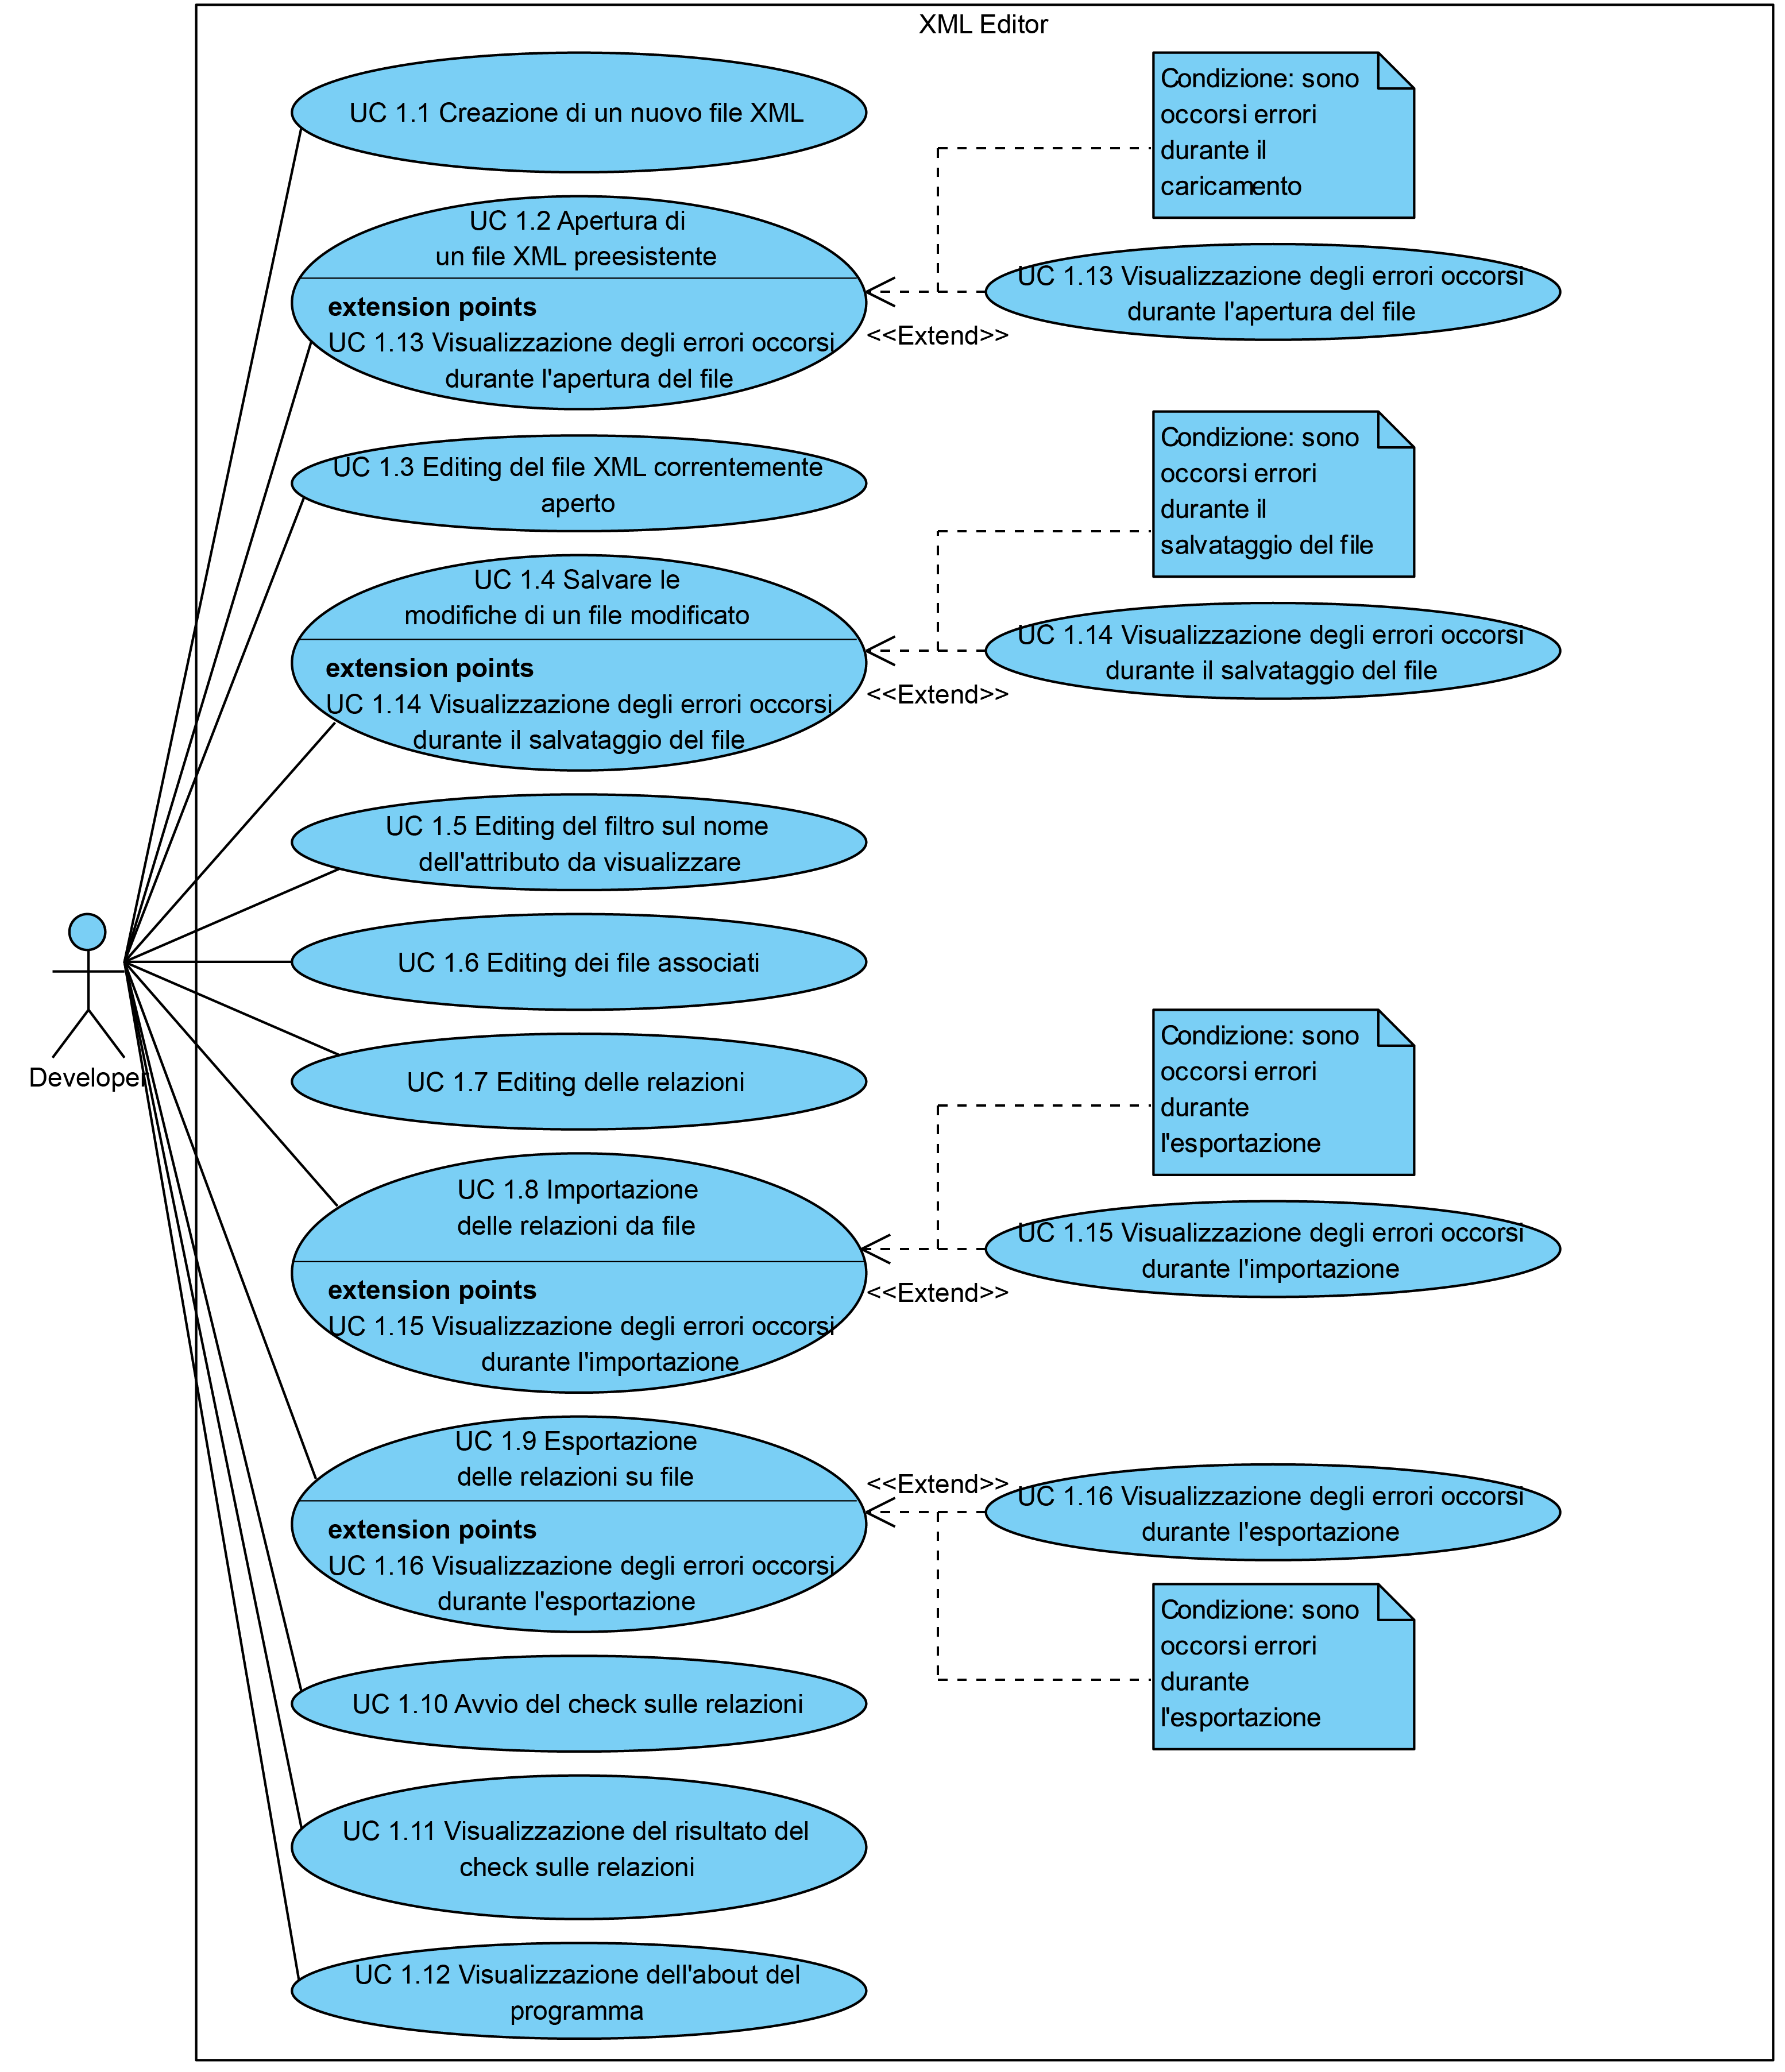
\includegraphics[width=0.9\columnwidth]{tool2/UC1.png} 
			\caption{Use Case - UC 1: Caso d'uso principale}
		\end{figure}
		
		\begin{itemize}
			\item\textbf{Attori}: developer.
			\item\textbf{Descrizione}: un developer deve avere tutte le funzionalità a disposizione per editare ed verificare uno o più file XML.
			\item\textbf{Precondizione}: il developer abbia lanciato il tool sotto un sistema Windows 7 o superiore.
			\item\textbf{Flusso principale degli eventi}: 
			\begin{enumerate}
				\item \textit{l'utente ha la possibilità di:} \textit{creazione di un nuovo file XML} (\hyperref[subsec:XEUC1.1]{UC 1.1});
				
				\item \textit{l'utente ha la possibilità di:} \textit{apertura di un file XML preesistente} (\hyperref[subsec:XEUC1.2]{UC 1.2});
				
				\item \textit{l'utente ha la possibilità di:} \textit{editing del file XML correntemente aperto} (\hyperref[subsec:XEUC1.3]{UC 1.3});
				
				\item \textit{l'utente ha la possibilità di:} \textit{salvare le modifiche di un file modificato} (\hyperref[subsec:XEUC1.4]{UC 1.4});
				
				\item \textit{l'utente ha la possibilità di:} \textit{editing del filtro sul nome dell'attributo da visualizzare} (\hyperref[subsec:XEUC1.5]{UC 1.5});
				
				\item \textit{l'utente ha la possibilità di:} \textit{editing dei file associati} (\hyperref[subsec:XEUC1.6]{UC 1.6});
				
				\item \textit{l'utente ha la possibilità di:} \textit{editing delle relazioni} (\hyperref[subsec:XEUC1.7]{UC 1.7});
				
				\item \textit{l'utente ha la possibilità di:} \textit{importazione delle relazioni da file} (\hyperref[subsec:XEUC1.8]{UC 1.8});
				
				\item \textit{l'utente ha la possibilità di:} \textit{esportazione delle relazioni su file} (\hyperref[subsec:XEUC1.9]{UC 1.9});
				
				\item \textit{l'utente ha la possibilità di:} \textit{avvio del check sulle relazioni} (\hyperref[subsec:XEUC1.10]{UC 1.10});
				
				\item \textit{l'utente ha la possibilità di:} \textit{visualizzazione del risultato del check sulle relazioni} (\hyperref[subsec:XEUC1.11]{UC 1.11});
				
				\item \textit{l'utente ha la possibilità di:} \textit{visualizzazione dell'about del programma} (\hyperref[subsec:XEUC1.12]{UC 1.12}).
				
			\end{enumerate}
			\item \textbf{Estensioni}
			\begin{enumerate}
				\item\textit{Visualizzazione degli errori occorsi durante l'apertura del file} (\hyperref[subsec:XEUC1.13]{UC 1.13});
				
				\item\textit{Visualizzazione degli errori occorsi durante il salvataggio del file} (\hyperref[subsec:XEUC1.14]{UC 1.14});
				
				\item\textit{Visualizzazione degli errori occorsi durante l'importazione} (\hyperref[subsec:XEUC1.15]{UC 1.15});
				
				\item\textit{Visualizzazione degli errori occorsi durante l'esportazione} (\hyperref[subsec:XEUC1.16]{UC 1.16}).
			\end{enumerate}
			\item\textbf{Postcondizione}: il sistema ha erogato le funzionalità richieste dal developer.
		\end{itemize}

	\subsection{UC 1.1: Creazione di un nuovo file XML}
		\label{subsec:XEUC1.1}
	
		\begin{figure}[!h] 
			\centering 
			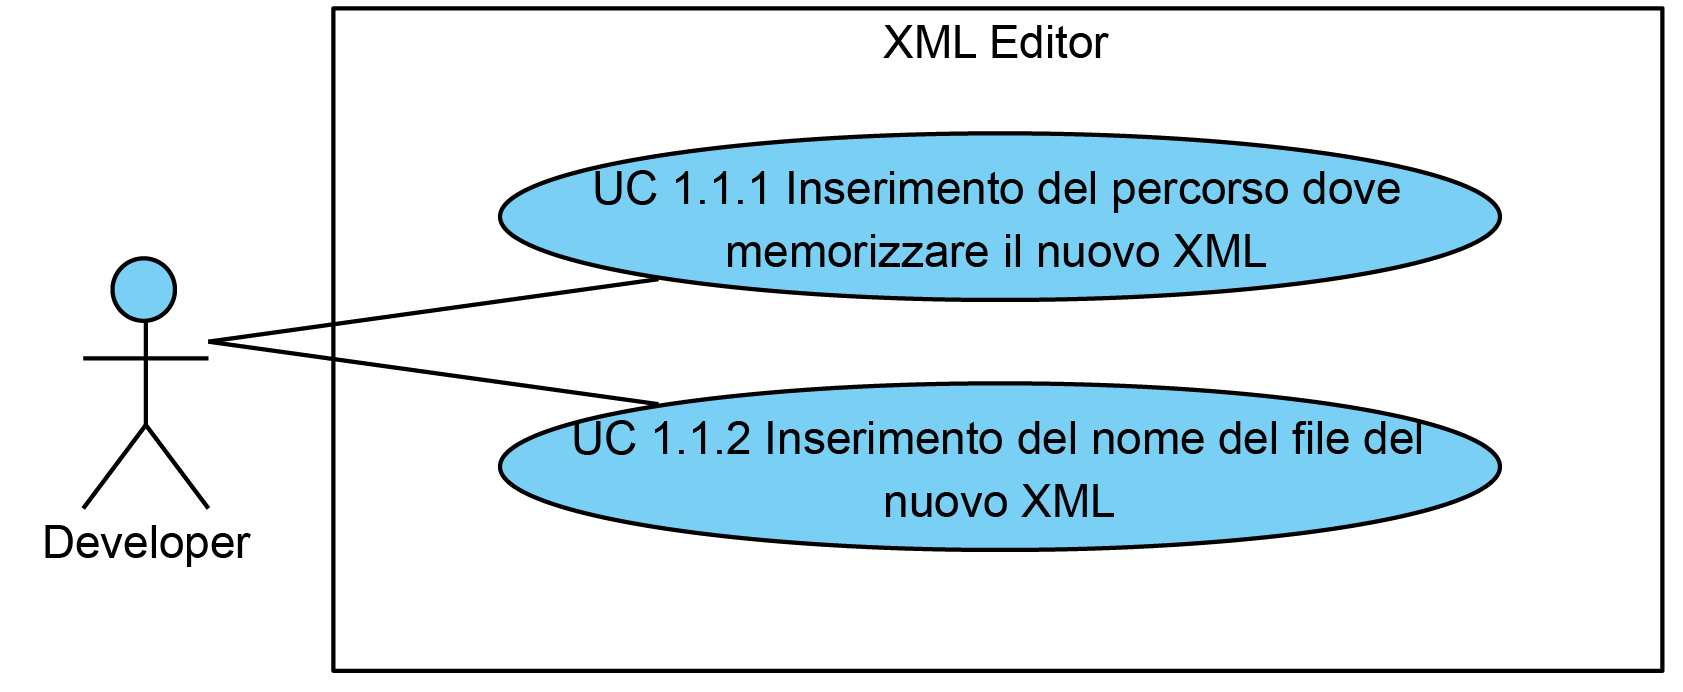
\includegraphics[width=0.9\columnwidth]{tool2/UC1-1.png} 
			\caption{Use Case - UC 1.1: Creazione di un nuovo file XML}
		\end{figure}
		
		\begin{itemize}
			\item\textbf{Attori}: developer.
			\item\textbf{Descrizione}: un developer deve poter creare un nuovo file XML.
			\item\textbf{Precondizione}: il developer ha lanciato il tool sotto un sistema Windows 7 o superiore.
			\item\textbf{Flusso principale degli eventi}: 
			\begin{enumerate}
				\item\textit{Inserimento del percorso dove memorizzare il nuovo XML} (\hyperref[subsec:XEUC1.1.1]{UC 1.1.1});
				\item\textit{Inserimento del nome del file del nuovo XML} (\hyperref[subsec:XEUC1.1.2]{UC 1.1.2}).
			\end{enumerate}
			\item\textbf{Postcondizione}: il sistema ha creato un nuovo file XML in memoria, esso sarà salvato su disco solo nel momento in cui l'utente lo salverà. Il sistema chiude il lavoro corrente e apre il nuovo file creato.
		\end{itemize}
		
	\subsection{UC 1.1.1: Inserimento del percorso dove memorizzare il nuovo XML}
		\label{subsec:XEUC1.1.1}
		
		\begin{itemize}
			\item\textbf{Attori}: developer.
			\item\textbf{Descrizione}: un developer deve poter inserire il percorso dove memorizzare su disco il nuovo file XML.
			\item\textbf{Precondizione}: il developer abbia selezionato l'azione per creare un nuovo file XML.
			\item\textbf{Scenario principale}: il developer sceglie il percorso dove memorizzare il nuovo file XML.
			\item\textbf{Postcondizione}: il sistema ha memorizzato il percorso dove salvare il nuovo file XML.
		\end{itemize}
		
	\subsection{UC 1.1.2: Inserimento del nome del file del nuovo XML}
		\label{subsec:XEUC1.1.2}
		
		\begin{itemize}
			\item\textbf{Attori}: developer.
			\item\textbf{Descrizione}: un developer deve poter inserire il nome del nuovo file XML.
			\item\textbf{Precondizione}: il developer abbia selezionato l'azione per creare un nuovo file XML.
			\item\textbf{Scenario principale}: il developer inserisce il nome del nuovo file XML.
			\item\textbf{Postcondizione}: il sistema ha memorizzato il nome del nuovo file XML.
		\end{itemize}
		
	\subsection{UC 1.2: Apertura di un file XML preesistente}
		\label{subsec:XEUC1.2}
		
		\begin{itemize}
			\item\textbf{Attori}: developer.
			\item\textbf{Descrizione}: un developer deve poter aprire un file XML preesistente.
			\item\textbf{Precondizione}: il developer abbia selezionato l'azione per aprire un file XML.
			\item\textbf{Scenario principale}: il developer inserisce il percorso ed il nome del file XML da aprire.
			\item\textbf{Postcondizione}: il sistema ha chiuso il lavoro precedentemente aperto e l'ha sostituito con il file XML selezionato. Se il file era stato precedentemente aperto ed erano stati settati alcuni file associati allora anche quei file saranno aperti.
		\end{itemize}
		
	\subsection{UC 1.3 Editing del file XML correntemente aperto}
		\label{subsec:XEUC1.3}
		
		\begin{figure}[!h] 
			\centering 
			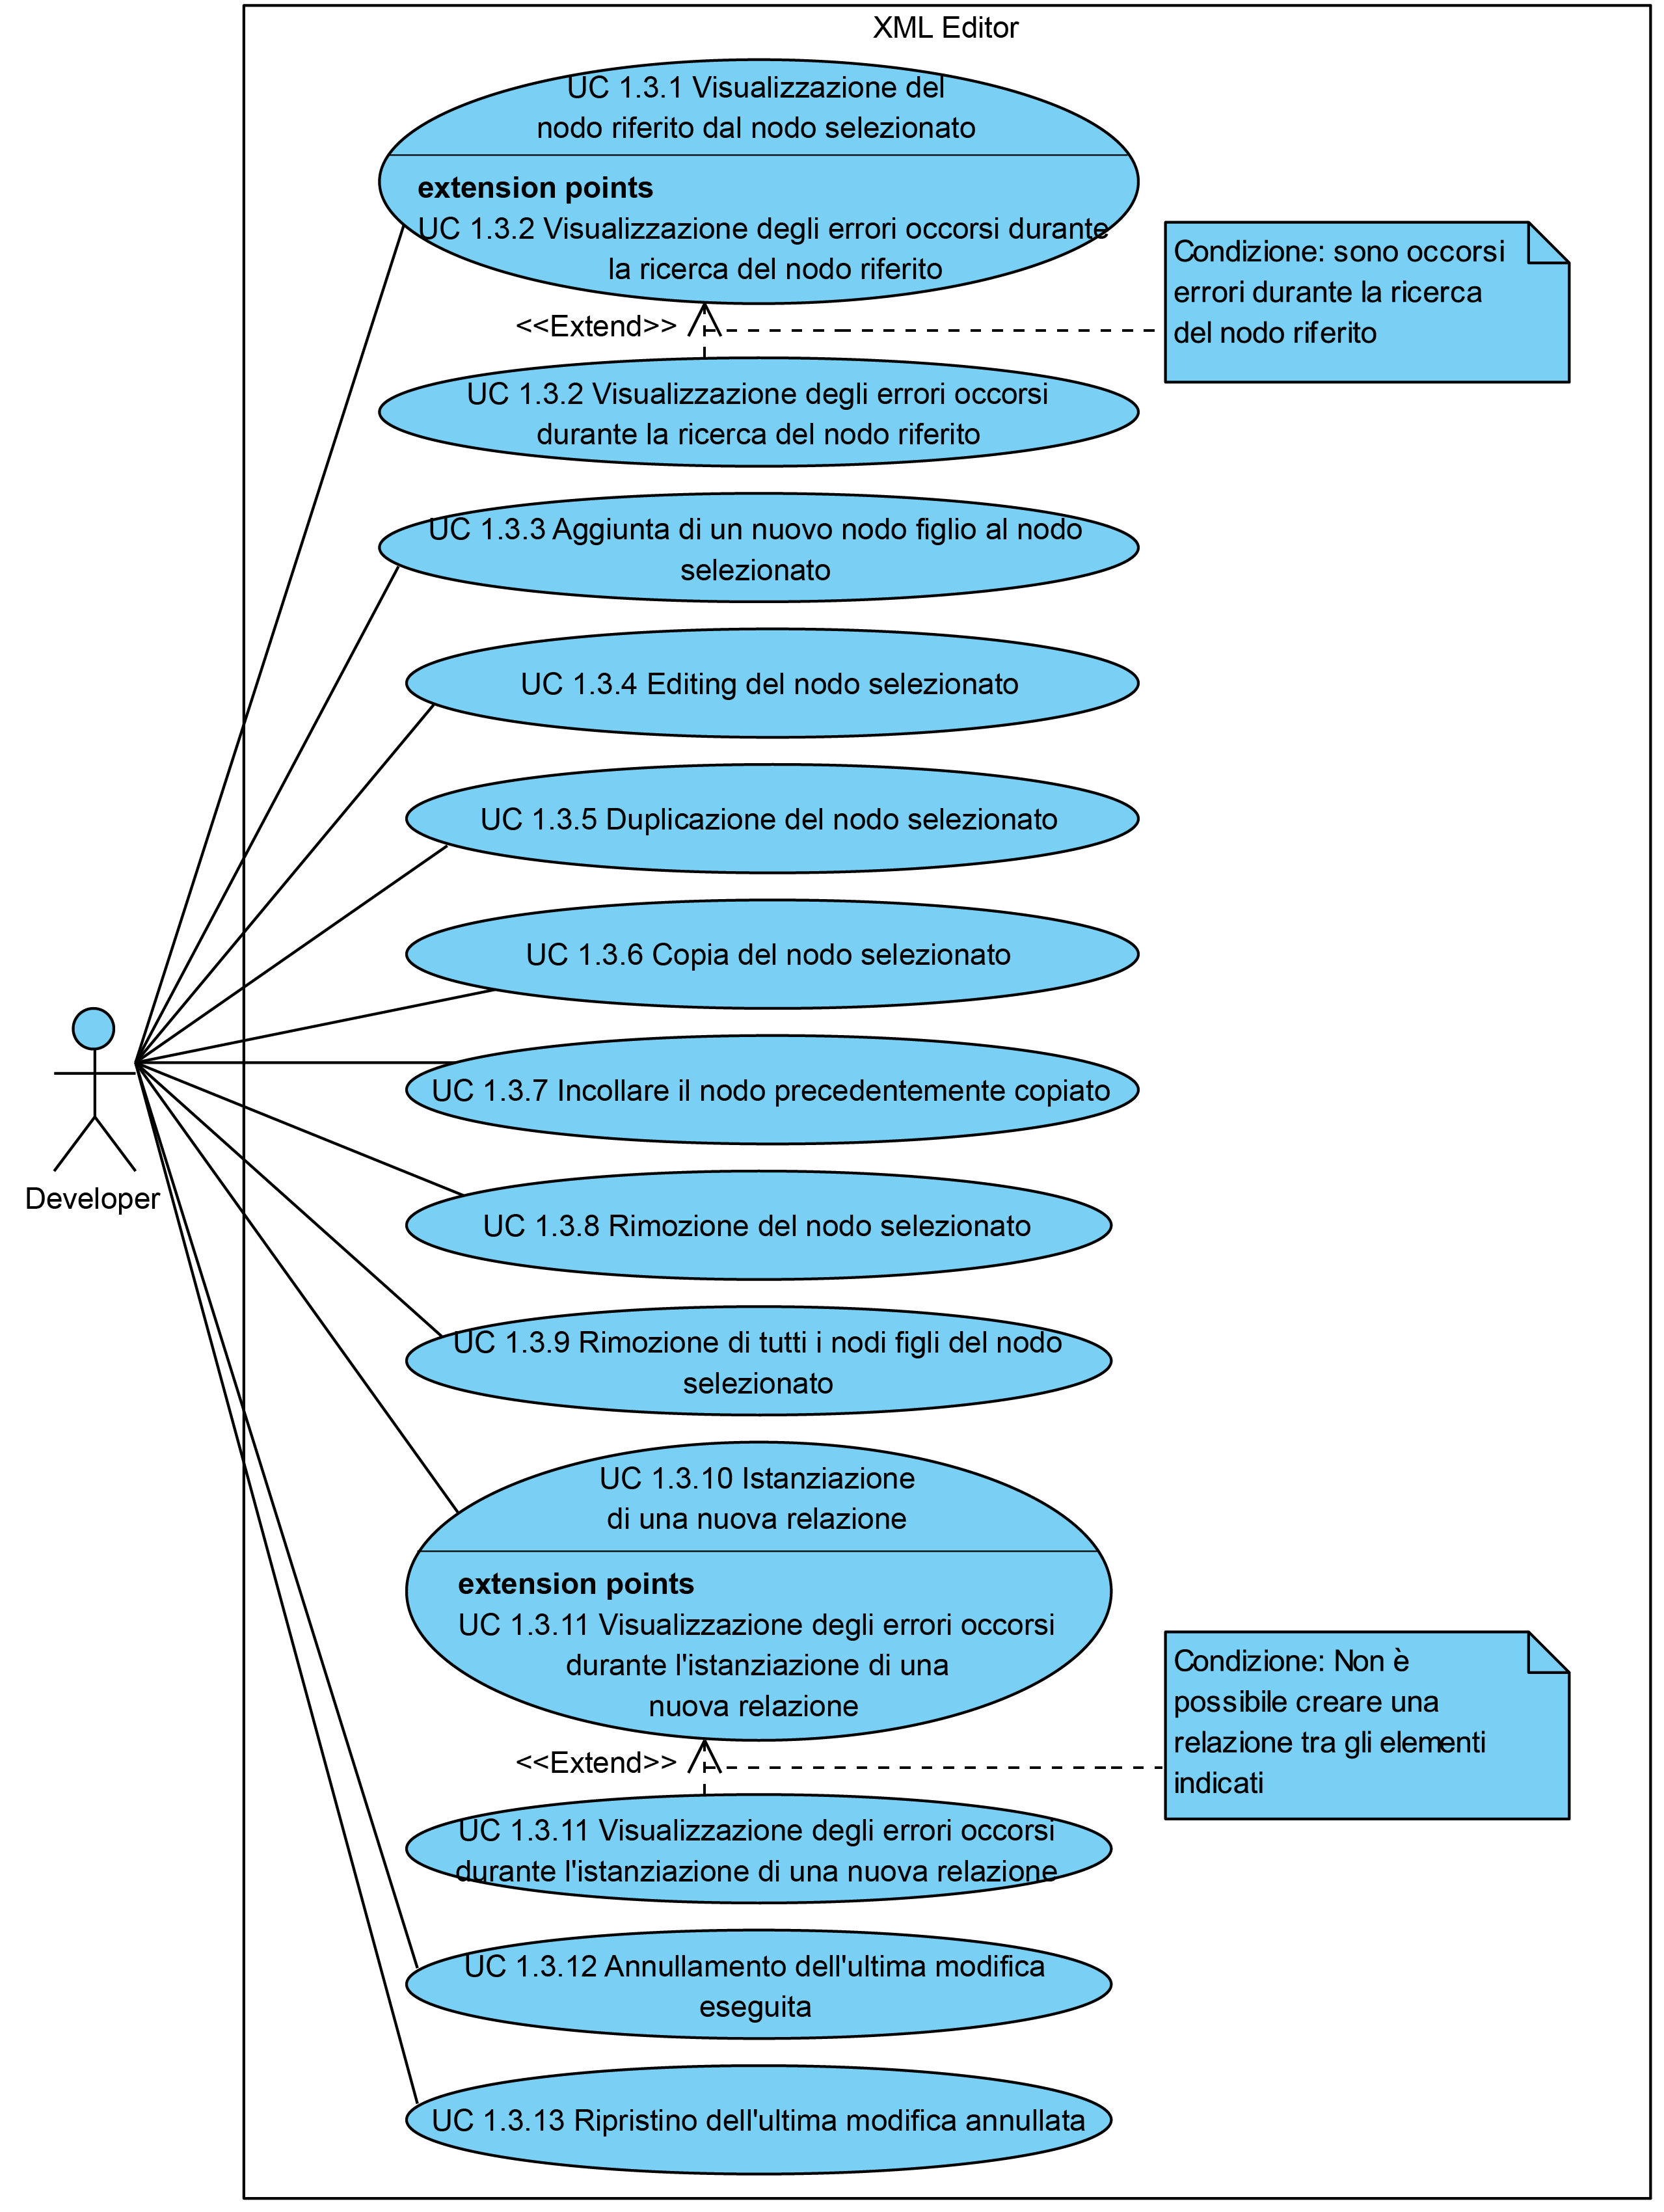
\includegraphics[width=0.9\columnwidth]{tool2/UC1-3.png} 
			\caption{Use Case - UC 1.3 Editing del file XML correntemente aperto}
		\end{figure}
		
		\begin{itemize}
			\item\textbf{Attori}: developer.
			\item\textbf{Descrizione}: un developer deve poter editare il file XML correntemente visualizzato.
			\item\textbf{Precondizione}: il developer abbia aperto con successo almeno un file XML.
			\item\textbf{Flusso principale degli eventi}: 
			\begin{enumerate}
				\item \textit{l'utente ha la possibilità di:} \textit{visualizzazione del nodo riferito dal nodo selezionato} (\hyperref[subsec:XEUC1.3.1]{UC 1.3.1});
				
				\item \textit{l'utente ha la possibilità di:} \textit{aggiunta di un nuovo nodo figlio al nodo selezionato} (\hyperref[subsec:XEUC1.3.3]{UC 1.3.3});
				
				\item \textit{l'utente ha la possibilità di:} \textit{editing del nodo selezionato} (\hyperref[subsec:XEUC1.3.4]{UC 1.3.4});
				
				\item \textit{l'utente ha la possibilità di:} \textit{duplicazione del nodo selezionato} (\hyperref[subsec:XEUC1.3.5]{UC 1.3.5});
				
				\item \textit{l'utente ha la possibilità di:} \textit{copia del nodo selezionato} (\hyperref[subsec:XEUC1.3.6]{UC 1.3.6});
				
				\item \textit{l'utente ha la possibilità di:} \textit{incollare il nodo precedentemente copiato} (\hyperref[subsec:XEUC1.3.7]{UC 1.3.7});
				
				\item \textit{l'utente ha la possibilità di:} \textit{rimozione del nodo selezionato} (\hyperref[subsec:XEUC1.3.8]{UC 1.3.8});
				
				\item \textit{l'utente ha la possibilità di:} \textit{rimozione di tutti i nodi figli del nodo selezionato} (\hyperref[subsec:XEUC1.3.9]{UC 1.3.9});
				
				\item \textit{l'utente ha la possibilità di:} \textit{istanziazione di una nuova relazione} (\hyperref[subsec:XEUC1.3.10]{UC 1.3.10});
				
				\item \textit{l'utente ha la possibilità di:} \textit{annullamento dell'ultima modifica eseguita} (\hyperref[subsec:XEUC1.3.12]{UC 1.3.12});
				
				\item \textit{l'utente ha la possibilità di:} \textit{ripristino dell'ultima modifica annullata} (\hyperref[subsec:XEUC1.3.13]{UC 1.3.13}).
				
			\end{enumerate}
			\item \textbf{Estensioni}
			\begin{enumerate}
				\item\textit{Visualizzazione degli errori occorsi durante la ricerca del nodo riferito} (\hyperref[subsec:XEUC1.3.2]{UC 1.3.2});
				
				\item\textit{Visualizzazione degli errori occorsi durante l'istanziazione di una nuova relazione} (\hyperref[subsec:XEUC1.16]{UC 1.3.11}).
			\end{enumerate}
			\item\textbf{Postcondizione}: il sistema ha modificato la versione caricata in memoria del file XML modificato.
		\end{itemize}
		
	\subsection{UC 1.3.1 Visualizzazione del nodo riferito dal nodo selezionato}
		\label{subsec:XEUC1.3.1}
		
		\begin{itemize}
			\item\textbf{Attori}: developer.
			\item\textbf{Descrizione}: un developer visualizza il nodo destinatario della relazione che ha il nodo selezionato come punto di partenza.
			\item\textbf{Precondizione}: il developer abbia selezionato l'azione per seguire la relazione.
			\item\textbf{Scenario principale}: il developer visualizza il nodo destinatario della relazione.
			\item\textbf{Postcondizione}: il sistema ha selezionato ed espanso l'albero fino al nodo destinatario della relazione. Se sono presenti più nodi destinazione o più relazioni da seguire viene sempre usata quella inserita precedentemente nel sistema.
		\end{itemize}
		
	\subsection{UC 1.3.2 Visualizzazione degli errori occorsi durante la ricerca del nodo riferito}
		\label{subsec:XEUC1.3.2}
		
		\begin{itemize}
			\item\textbf{Attori}: developer.
			\item\textbf{Descrizione}: si è verificato uno dei seguenti errori durante la ricerca del nodo destinazione:
			\begin{itemize}
				\item non esiste nessuna relazione per cui il nodo selezionato è riconoscibile come nodo partenza di una relazione;
				\item non esiste nessun nodo di destinazione.
			\end{itemize}
			\item\textbf{Precondizione}: il developer ha avviato l'azione per mostrare il nodo destinatario della relazione.
			\item\textbf{Scenario principale}: viene fornita una spiegazione dell'errore commesso e come risolverlo.
			\item\textbf{Postcondizione}: l'errore commesso è stato visualizzato e spiegato, non viene visualizzato nessun nodo destinazione.
		\end{itemize}
		
	\subsection{UC 1.3.3 Aggiunta di un nuovo nodo figlio al nodo selezionato}
		\label{subsec:XEUC1.3.3}
			
		\begin{itemize}
			\item\textbf{Attori}: developer.
			\item\textbf{Descrizione}: viene aggiunto un nuovo nodo vuoto come figlio del nodo correttamente selezionato.
			\item\textbf{Precondizione}: il developer abbia selezionato l'azione aggiungere un nuovo nodo come figlio del nodo correttamente visualizzato.
			\item\textbf{Scenario principale}: il developer inserisce il tag name del nuovo nodo.
			\item\textbf{Postcondizione}: il sistema ha selezionato il nodo ed espanso l'albero fino al nuovo nodo creato.
		\end{itemize}
		
	\subsection{UC 1.3.4 Editing del nodo selezionato}
		\label{subsec:XEUC1.3.4}
		
		\begin{figure}[!h] 
			\centering 
			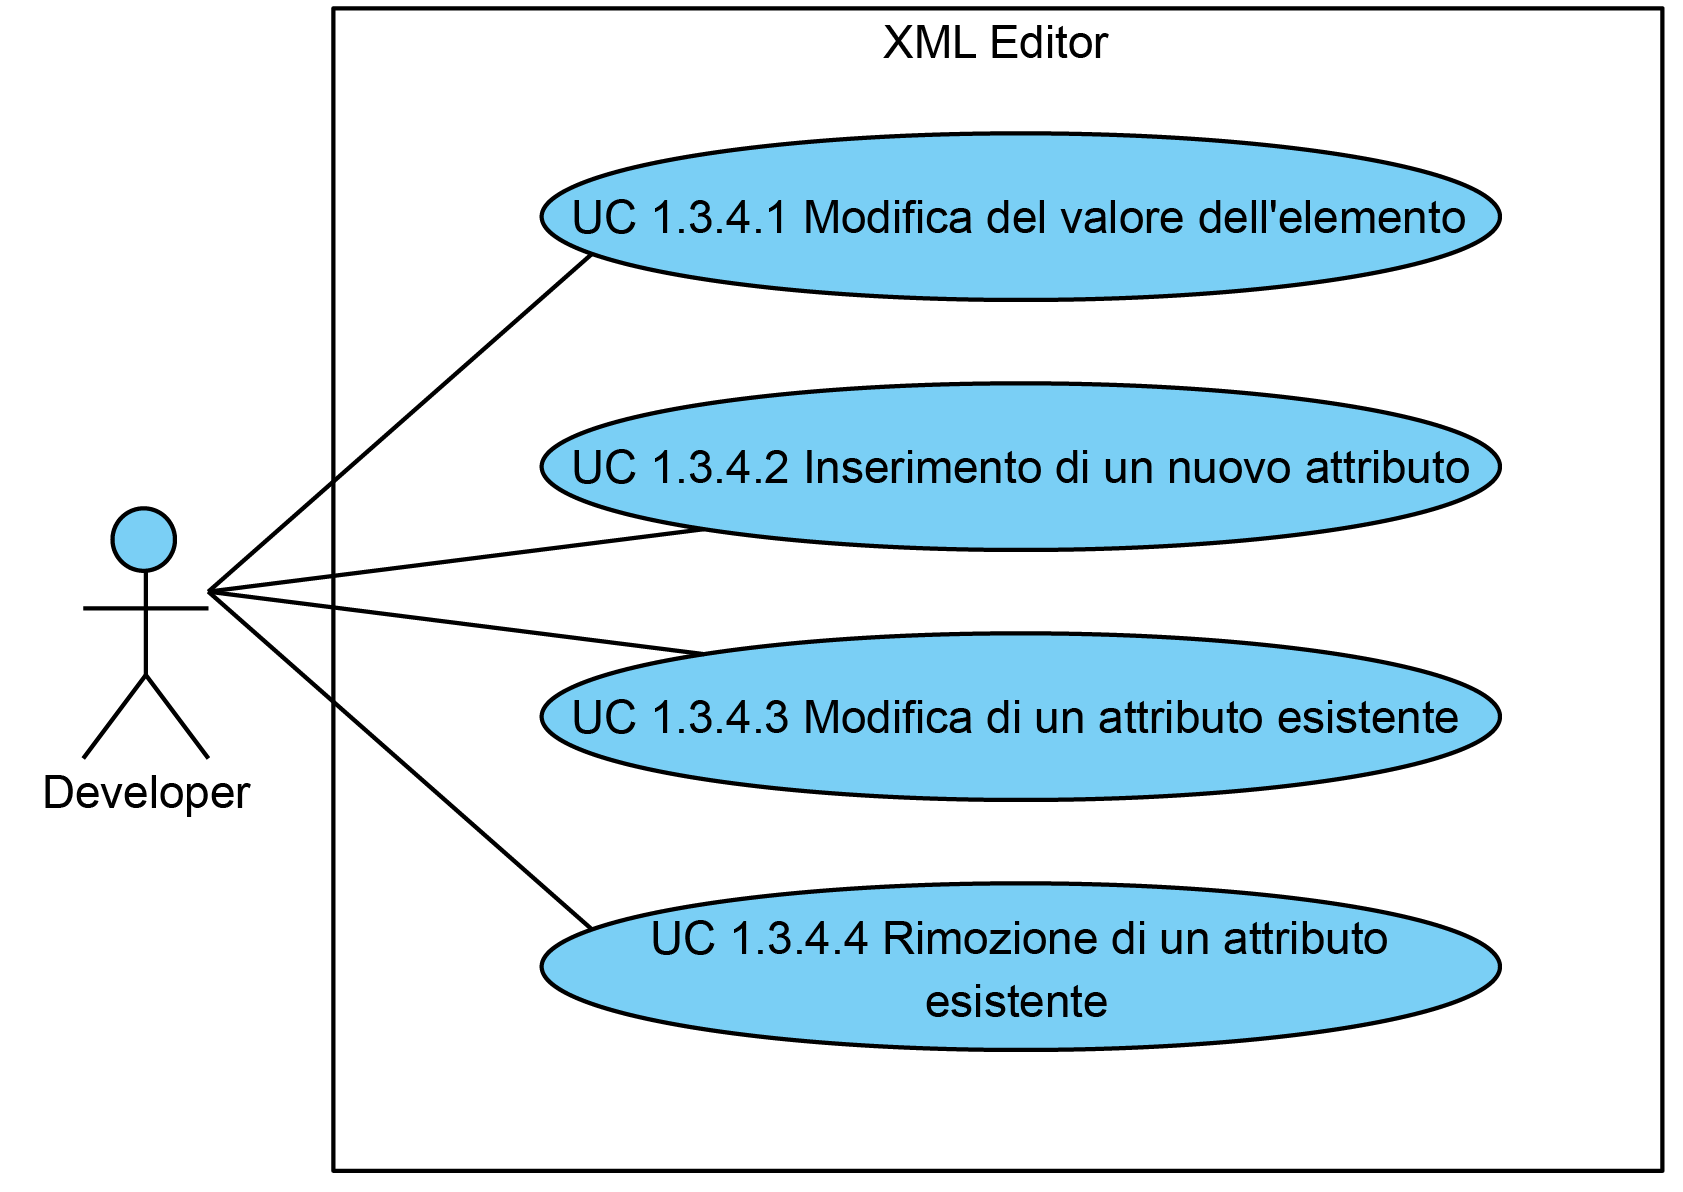
\includegraphics[width=0.9\columnwidth]{tool2/UC1-3-4.png} 
			\caption{Use Case - UC 1.3.4 Editing del nodo selezionato}
		\end{figure}
		
		\begin{itemize}
			\item\textbf{Attori}: developer.
			\item\textbf{Descrizione}: un developer deve poter editare il file XML correntemente visualizzato.
			\item\textbf{Precondizione}: il developer abbia selezionato l'azione per modificare l'elemento correntemente selezionato.
			\item\textbf{Flusso principale degli eventi}: 
			\begin{enumerate}
				\item \textit{l'utente ha la possibilità di:} \textit{modifica del valore dell'elemento} (\hyperref[subsec:XEUC1.3.4.1]{UC 1.3.4.1});
				
				\item \textit{l'utente ha la possibilità di:} \textit{inserimento di un nuovo attributo} (\hyperref[subsec:XEUC1.3.4.2]{UC 1.3.4.2});
				
				\item \textit{l'utente ha la possibilità di:} \textit{modifica di un attributo esistente} (\hyperref[subsec:XEUC1.3.4.3]{UC 1.3.4.3});
				
				\item \textit{l'utente ha la possibilità di:} \textit{rimozione di un attributo esistente} (\hyperref[subsec:XEUC1.3.4.4]{UC 1.3.4}).
				
			\end{enumerate}
			\item\textbf{Postcondizione}: il sistema ha modificato la versione caricata in memoria del file XML modificato.
		\end{itemize}
		
	\subsection{UC 1.3.4.1 Modifica del valore dell'elemento}
		\label{subsec:XEUC1.3.4.1}
		
		\begin{itemize}
			\item\textbf{Attori}: developer.
			\item\textbf{Descrizione}: il developer può modificare il valore dell'elemento.
			\item\textbf{Precondizione}: il developer abbia selezionato l'azione aggiungere per modificare un elemento.
			\item\textbf{Scenario principale}: il developer inserisce il nuovo value.
			\item\textbf{Postcondizione}: il sistema ha modificato il valore dell'elemento.
		\end{itemize}
		
	\subsection{UC 1.3.4.2 Inserimento di un nuovo attributo}
		\label{subsec:XEUC1.3.4.2}
		
		\begin{itemize}
			\item\textbf{Attori}: developer.
			\item\textbf{Descrizione}: il developer può aggiungere un attributo all'elemento.
			\item\textbf{Precondizione}: il developer abbia selezionato l'azione aggiungere per modificare un elemento.
			\item\textbf{Scenario principale}: il developer inserisce il nome del nuovo attributo ed il corrispettivo valore.
			\item\textbf{Postcondizione}: il sistema ha aggiunto un nuovo attributo con il nome ed il valore inseriti dal developer.
		\end{itemize}
		
	\subsection{UC 1.3.4.3 Modifica di un attributo esistente}
		\label{subsec:XEUC1.3.4.3}
		
		\begin{itemize}
			\item\textbf{Attori}: developer.
			\item\textbf{Descrizione}: il developer può modificare il valore e/o il nome di un attributo precedentemente inserito.
			\item\textbf{Precondizione}: il developer abbia selezionato l'azione aggiungere per modificare un elemento.
			\item\textbf{Scenario principale}: il developer inserisce il nome e/o il valore dell'attributo da modificare.
			\item\textbf{Postcondizione}: il sistema ha modificato l'attributo selezionato con i dati inseriti dal developer.
		\end{itemize}
		
	\subsection{UC 1.3.4.4 Rimozione di un attributo esistente}
		\label{subsec:XEUC1.3.4.4}
		
		\begin{itemize}
			\item\textbf{Attori}: developer.
			\item\textbf{Descrizione}: il developer può eliminare un attributo precedentemente inserito.
			\item\textbf{Precondizione}: il developer abbia selezionato l'azione aggiungere per modificare un elemento.
			\item\textbf{Scenario principale}: il developer seleziona l'attributo da eliminare.
			\item\textbf{Postcondizione}: il sistema ha eliminato l'attributo selezionato dal developer.
		\end{itemize}
		
	\subsection{UC 1.3.5 Duplicazione del nodo selezionato}
		\label{subsec:XEUC1.3.5}
		
		\begin{itemize}
			\item\textbf{Attori}: developer.
			\item\textbf{Descrizione}: viene aggiunta al padre del nodo selezionato una copia profonda di questo.
			\item\textbf{Precondizione}: il developer abbia selezionato l'azione di duplicazione di un nodo.
			\item\textbf{Scenario principale}: il developer seleziona il nodo da duplicare.
			\item\textbf{Postcondizione}: il sistema ha aggiunto al padre del nodo selezionato una copia profonda di tale nodo. Inoltre ha espanso l'albero fino al nuovo nodo creato.
		\end{itemize}
		
	\subsection{UC 1.3.6 Copia del nodo selezionato}
		\label{subsec:XEUC1.3.6}
		
		\begin{itemize}
			\item\textbf{Attori}: developer.
			\item\textbf{Descrizione}: viene fatta una copia profonda del nodo selezionato e conservata in memoria, pronta per essere incollata.
			\item\textbf{Precondizione}: il developer abbia selezionato l'azione di copia di un nodo.
			\item\textbf{Scenario principale}: il developer seleziona il nodo che intende copia.
			\item\textbf{Postcondizione}: il sistema ha memorizzato in memoria una copia profonda del nodo selezionato.
		\end{itemize}
		
	\subsection{UC 1.3.7 Incollare il nodo precedentemente copiato}
		\label{subsec:XEUC1.3.7}
		
		\begin{itemize}
			\item\textbf{Attori}: developer.
			\item\textbf{Descrizione}: viene aggiunto come figlio del nodo correttamente selezionato il nodo precedentemente copiato.
			\item\textbf{Precondizione}: il developer richiede di copiare il nodo precedentemente copiato.
			\item\textbf{Scenario principale}: il developer seleziona il nodo destinazione che conterrà il nuovo nodo.
			\item\textbf{Postcondizione}: il sistema ha aggiunto come figlio del nodo destinazione il nodo precedentemente copiato. Inoltre ha selezionato ed espanso l'albero fino al nuovo nodo aggiunto.
		\end{itemize}
		
	\subsection{UC 1.3.8 Rimozione del nodo selezionato}
		\label{subsec:XEUC1.3.8}
		
		\begin{itemize}
			\item\textbf{Attori}: developer.
			\item\textbf{Descrizione}: viene rimosso il nodo correntemente selezionato.
			\item\textbf{Precondizione}: il developer abbia selezionato l'azione di rimozione di un nodo.
			\item\textbf{Scenario principale}: il developer abbia selezionato il nodo da rimuovere.
			\item\textbf{Postcondizione}: il sistema ha rimosso il nodo selezionato.
		\end{itemize}
		
	\subsection{UC 1.3.9 Rimozione di tutti i nodi figli del nodo selezionato}
		\label{subsec:XEUC1.3.9}
		
		\begin{itemize}
			\item\textbf{Attori}: developer.
			\item\textbf{Descrizione}: vengono rimossi tutti i nodi figli del nodo correntemente selezionato.
			\item\textbf{Precondizione}: il developer abbia selezionato l'azione per rimuovere tutti i nodi figli.
			\item\textbf{Scenario principale}: il developer seleziona il nodo di cui si vuole rimuovere tutti i figli.
			\item\textbf{Postcondizione}: il sistema ha rimosso tutti i nodi del nodo attualmente selezionato.
		\end{itemize}
		
	\subsection{UC 1.3.10 Istanziazione di una nuova relazione}
		\label{subsec:XEUC1.3.10}
		
		\begin{itemize}
			\item\textbf{Attori}: developer.
			\item\textbf{Descrizione}: vengono creati in automatico tutti i nodi necessari per creare una relazione tra i nodi partenza selezionati e il nodo destinatario scelto.
			\item\textbf{Precondizione}: il developer abbia selezionato l'azione per creare in automatico una relazione.
			\item\textbf{Scenario principale}: il developer seleziona uno o più nodi e successivamente sceglie il nodo che riferirà i nodi precedentemente selezionati.
			\item\textbf{Postcondizione}: il sistema ha creato tutti i nodi necessari ad esplicitare le relazioni richieste.
		\end{itemize}
		
	\subsection{UC 1.3.11 Visualizzazione degli errori occorsi durante l'istanziazione di una nuova relazione}
		\label{subsec:XEUC1.3.11}
		
		\begin{itemize}
			\item\textbf{Attori}: developer.
			\item\textbf{Descrizione}: si è verificato uno dei seguenti errori durante l'istanziazione di una relazione:
			\begin{itemize}
				\item non esiste nessuna relazione per cui il nodo selezionato è riconoscibile come nodo partenza di una relazione;
				\item sono stati selezionati come nodi destinazione nodi non riconoscibili come destinazione di una relazione.
				\item non esiste nessun percorso di relazioni che lega il nodo partenza con il nodo destinazione selezionati;
				\item sono stati selezionati come nodi destinazione nodi di tipi differenti.
			\end{itemize}.
			\item\textbf{Precondizione}: il developer ha selezionato l'azione per creare una nuova relazione e specificato gli elementi da coinvolgere.
			\item\textbf{Scenario principale}: viene fornita una spiegazione dell'errore commesso e come risolverlo.
			\item\textbf{Postcondizione}: l'errore commesso è stato visualizzato e spiegato, non viene eseguita nessuna modifica al file XML.
		\end{itemize}
		
	\subsection{UC 1.3.12 Annullamento dell'ultima modifica eseguita}
		\label{subsec:XEUC1.3.12}
		
		\begin{itemize}
			\item\textbf{Attori}: developer.
			\item\textbf{Descrizione}: viene annullata l'ultima modifica e ripristinato lo stato precedente del file.
			\item\textbf{Precondizione}: il developer abbia selezionato l'azione per annullare l'ultima modifica ed è stata effettuata almeno una modifica al file XML.
			\item\textbf{Scenario principale}: viene ripristinato lo stato del file precedente alla modifica.
			\item\textbf{Postcondizione}: il sistema ha ripristinato lo stato del file prima dell'ultima azione di modifica.
		\end{itemize}
		
	\subsection{UC 1.3.13 Ripristino dell'ultima modifica annullata}
		\label{subsec:XEUC1.3.13}
		
		\begin{itemize}
			\item\textbf{Attori}: developer.
			\item\textbf{Descrizione}: viene ripristinata l'ultima modifica annullata.
			\item\textbf{Precondizione}: il developer abbia selezionato l'azione per ripristinare l'ultima modifica annullata ed è stata annullata almeno una modifica al file XML.
			\item\textbf{Scenario principale}: viene ripristinata l'ultima modifica annullata.
			\item\textbf{Postcondizione}: il sistema ha ripristinato lo stato del file prima dell'ultima azione di annullamento eseguita.
		\end{itemize}
		
	\subsection{UC 1.4 Salvare le modifiche di un file modificato}
		\label{subsec:XEUC1.4}
			
		\begin{itemize}
			\item\textbf{Attori}: developer.
			\item\textbf{Descrizione}: un developer deve poter salvare le modifiche effettuate su un file XML precedentemente aperto.
			\item\textbf{Precondizione}: il developer abbia selezionato l'azione per salvare un file XML e abbia almeno un file aperto e modificato.
			\item\textbf{Scenario principale}: viene salvato il file XML modificato.
			\item\textbf{Postcondizione}: il sistema ha salvato su disco le modifiche apportate al file XML.
		\end{itemize}
		
	\subsection{UC 1.5 Editing del filtro sul nome dell'attributo da visualizzare}
		\label{subsec:XEUC1.5}
		
		\begin{itemize}
			\item\textbf{Attori}: developer.
			\item\textbf{Descrizione}: un developer deve poter modificare il filtro che seleziona l'attributo cui valore è mostrato nell'albero rappresentante il file XML.
			\item\textbf{Precondizione}: il developer abbia lanciato il tool sotto un sistema Windows 7 o superiore.
			\item\textbf{Scenario principale}: il developer inserisce il nuovo filtro.
			\item\textbf{Postcondizione}: il sistema ha salvato il nuovo filtro e ha aggiornato la visualizzazione di tutti i file aperti.
		\end{itemize}
		
	\subsection{UC 1.6 Editing dei file associati}
		\label{subsec:XEUC1.6}
		
		\begin{figure}[!h] 
			\centering 
			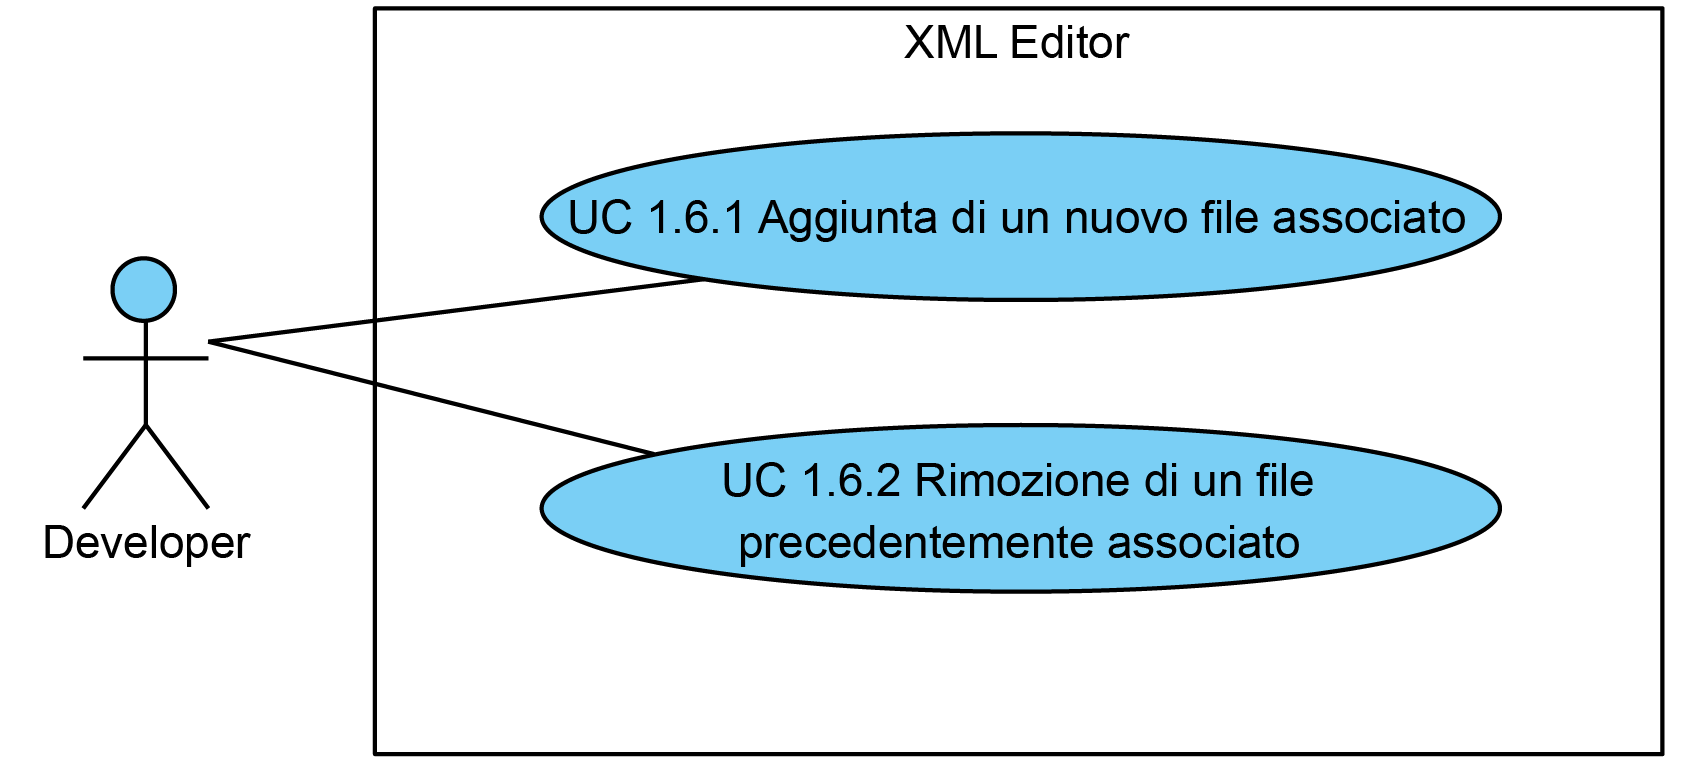
\includegraphics[width=0.9\columnwidth]{tool2/UC1-6.png} 
			\caption{Use Case - UC 1.6 Editing dei file associati}
		\end{figure}
		
		\begin{itemize}
			\item\textbf{Attori}: developer.
			\item\textbf{Descrizione}: un developer deve poter aggiungere e rimuovere i file associati.
			\item\textbf{Precondizione}: il developer ha caricato correttamente un file XML.
			\item\textbf{Flusso principale degli eventi}: 
			\begin{enumerate}
				\item \textit{l'utente ha la possibilità di:} \textit{aggiunta di un nuovo file associato} (\hyperref[subsec:XEUC1.6.1]{UC 1.6.1});
				
				\item \textit{l'utente ha la possibilità di:} \textit{rimozione di un file precedentemente associato} (\hyperref[subsec:XEUC1.6.2]{UC1.6.2}).
				
			\end{enumerate}
			\item\textbf{Postcondizione}: il sistema ha modificato i file associati del file XML principale attualmente aperto.
		\end{itemize}
		
	\subsection{UC 1.6.1 Aggiunta di un nuovo file associato}
		\label{subsec:XEUC1.6.1}
		
		\begin{itemize}
			\item\textbf{Attori}: developer.
			\item\textbf{Descrizione}: un developer deve poter aggiungere un nuovo file associato al corrente file principale.
			\item\textbf{Precondizione}: il developer abbia selezionato l'azione di modifica dei file associati.
			\item\textbf{Scenario principale}: il developer inserisce il percorso ed il nome del nuovo file associato.
			\item\textbf{Postcondizione}: il sistema ha salvato il nuovo file associato lo carica.
		\end{itemize}
		
	\subsection{UC 1.6.2 Rimozione di un file precedentemente associato}
		\label{subsec:XEUC1.6.2}
		
		\begin{itemize}
			\item\textbf{Attori}: developer.
			\item\textbf{Descrizione}: un developer deve poter rimuovere un file associato dal corrente file principale.
			\item\textbf{Precondizione}: il developer abbia selezionato l'azione di modifica dei file associati.
			\item\textbf{Scenario principale}: il developer seleziona il file da rimuovere.
			\item\textbf{Postcondizione}: il sistema ha rimosso il file selezionato. La copia in memoria del file non è stata eliminata.
		\end{itemize}
		
	\subsection{UC 1.7 Editing delle relazioni}
		\label{subsec:XEUC1.7}
		
		\begin{figure}[!h] 
			\centering 
			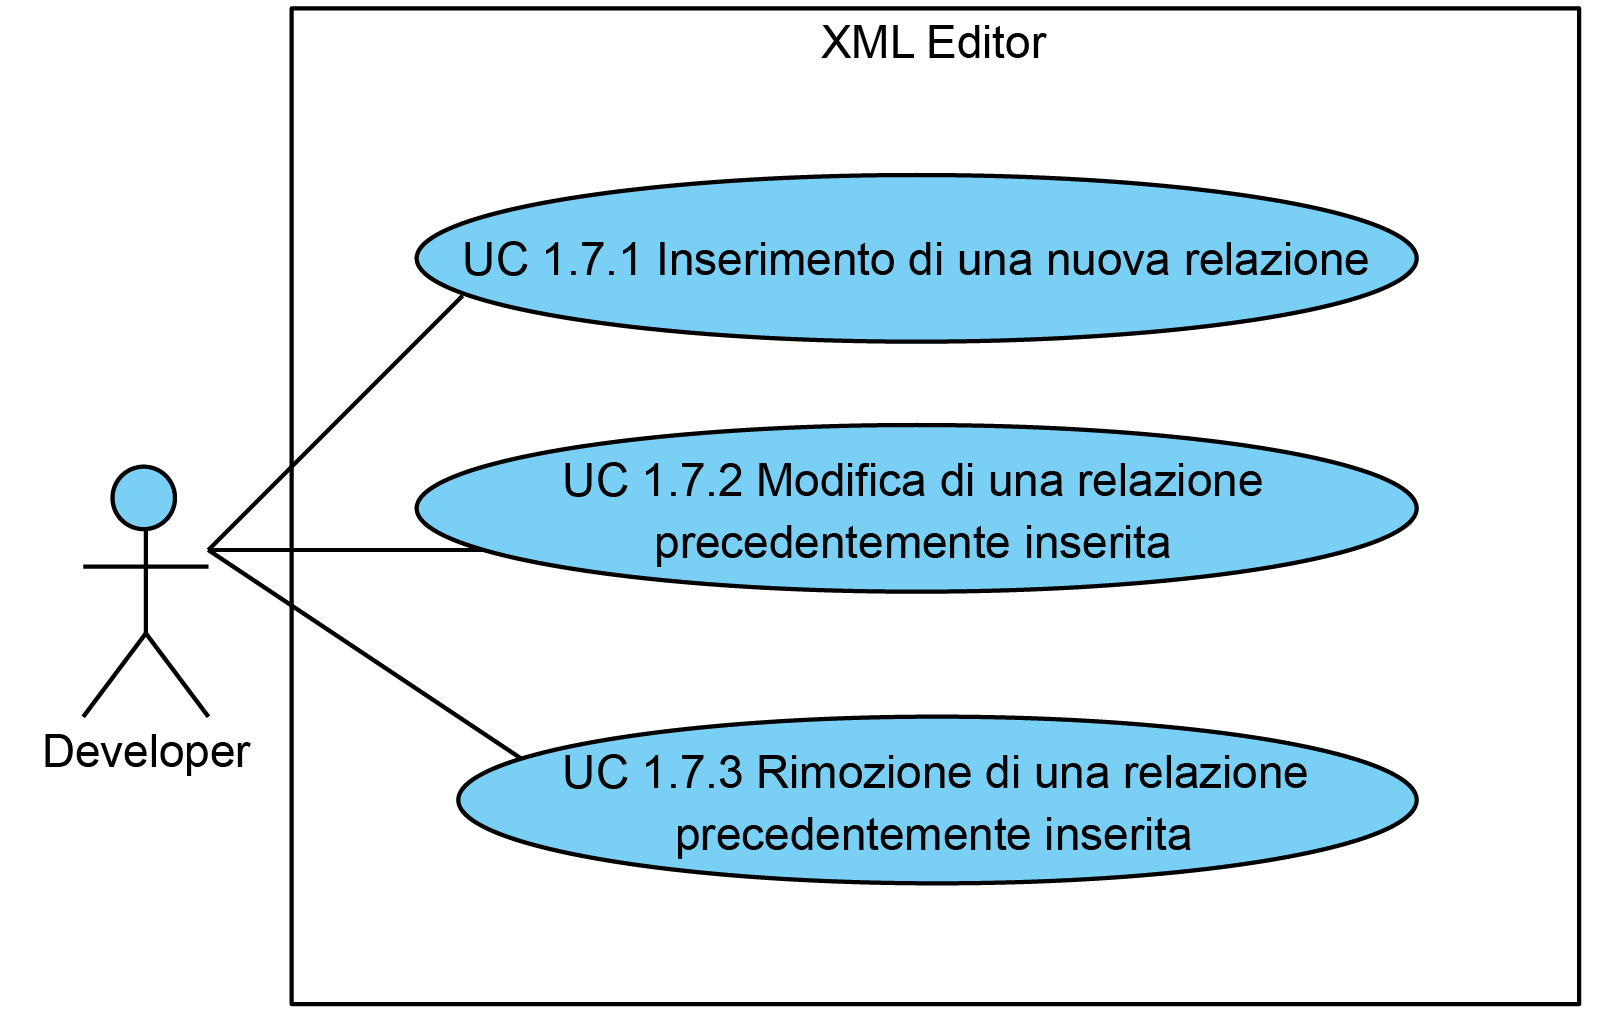
\includegraphics[width=0.9\columnwidth]{tool2/UC1-7.png} 
			\caption{Use Case - UC 1.7 Editing delle relazioni}
		\end{figure}
		
		\begin{itemize}
			\item\textbf{Attori}: developer.
			\item\textbf{Descrizione}: un developer deve poter editare le relazioni presenti.
			\item\textbf{Precondizione}: il developer ha lanciato il tool sotto un sistema Windows 7 o superiore.
			\item\textbf{Flusso principale degli eventi}: 
			\begin{enumerate}
				\item \textit{l'utente ha la possibilità di:} \textit{inserimento di una nuova relazione} (\hyperref[subsec:XEUC1.7.1]{UC 1.7.1});
				
				\item \textit{l'utente ha la possibilità di:} \textit{modifica di una relazione precedentemente inserita} (\hyperref[subsec:XEUC1.7.2]{UC1.7.2});
				
				\item \textit{l'utente ha la possibilità di:} \textit{rimozione di una relazione precedentemente inserita} (\hyperref[subsec:XEUC1.7.3]{UC1.7.3}).
				
			\end{enumerate}
			\item\textbf{Postcondizione}: il sistema ha modificato le relazione come desiderato dall'utente.
		\end{itemize}
		
	\subsection{UC 1.7.1 Inserimento di una nuova relazione}
		\label{subsec:XEUC1.7.1}
		
		\begin{itemize}
			\item\textbf{Attori}: developer.
			\item\textbf{Descrizione}: un developer deve poter aggiungere una nuova relazione.
			\item\textbf{Precondizione}: il developer abbia selezionato l'azione di modifica delle relazioni.
			\item\textbf{Scenario principale}: il developer inserisce tutte le informazioni necessarie alla creazione di una relazione.
			\item\textbf{Postcondizione}: il sistema ha memorizzato la nuova relazione.
		\end{itemize}
		
	\subsection{UC 1.7.2 Modifica di una relazione precedentemente inserita}
		\label{subsec:XEUC1.7.2}
		
		\begin{itemize}
			\item\textbf{Attori}: developer.
			\item\textbf{Descrizione}: un developer deve poter modificare una relazione precedentemente inserita.
			\item\textbf{Precondizione}: il developer abbia selezionato l'azione di modifica delle relazioni e la relazione da modificare.
			\item\textbf{Scenario principale}: il developer inserisce tutte le informazioni che vuole modificare della relazione.
			\item\textbf{Postcondizione}: il sistema ha memorizzato i cambiamenti nella relazione selezionata.
		\end{itemize}
		
	\subsection{UC 1.7.3 Rimozione di una relazione precedentemente inserita}
		\label{subsec:XEUC1.7.3}
		
		\begin{itemize}
			\item\textbf{Attori}: developer.
			\item\textbf{Descrizione}: un developer deve poter rimuovere una relazione.
			\item\textbf{Precondizione}: il developer abbia selezionato l'azione di modifica delle relazioni.
			\item\textbf{Scenario principale}: il developer seleziona la relazione da rimuovere.
			\item\textbf{Postcondizione}: il sistema ha rimosso la relazione selezionata.
		\end{itemize}
		
	\subsection{UC 1.8 Importazione delle relazioni da file}
		\label{subsec:XEUC1.8}
		
		\begin{itemize}
			\item\textbf{Attori}: developer.
			\item\textbf{Descrizione}: un developer deve poter importare e sostituire le relazioni correnti con le relazione contenute in un file di configurazione precedentemente esportato.
			\item\textbf{Precondizione}: il developer ha selezionato l'azione per importare le relazioni da un file.
			\item\textbf{Scenario principale}: il developer inserisce il percorso ed il nome del file contenente le relazioni.
			\item\textbf{Postcondizione}: il sistema ha rimosso tutte le precedenti relazioni e le ha sostituite con tutte quelle presenti nel file.
		\end{itemize}
		
	\subsection{UC 1.9 Esportazione delle relazioni su file}
		\label{subsec:XEUC1.9}
		
		\begin{itemize}
			\item\textbf{Attori}: developer.
			\item\textbf{Descrizione}: un developer deve poter esportare le relazioni attualmente inserite su file.
			\item\textbf{Precondizione}: il developer ha selezionato l'azione per esportare le relazioni su file.
			\item\textbf{Scenario principale}: il developer inserisce il percorso ed il nome del file dove esportare le relazioni.
			\item\textbf{Postcondizione}: il sistema esportato le relazioni nel file selezionato.
		\end{itemize}
		
	\subsection{UC 1.10 Avvio del check sulle relazioni}
		\label{subsec:XEUC1.10}
		
		\begin{itemize}
			\item\textbf{Attori}: developer.
			\item\textbf{Descrizione}: un developer deve poter verificare la consistenza delle relazioni presenti nel file principale e in tutti i file associati sulla base delle relazioni inserite.
			\item\textbf{Precondizione}: il developer ha selezionato l'azione per verificare la consistenza delle relazioni. Almeno un file XML deve essere stato aperto con successo.
			\item\textbf{Scenario principale}: il developer seleziona l'azione per effettuare il check delle relazioni.
			\item\textbf{Postcondizione}: il sistema ha verificato le relazioni nel file principale e in tutti gli associati.
		\end{itemize}
		
	\subsection{UC 1.11 Visualizzazione del risultato del check sulle relazioni}
		\label{subsec:XEUC1.11}
		
		\begin{figure}[!h] 
			\centering 
			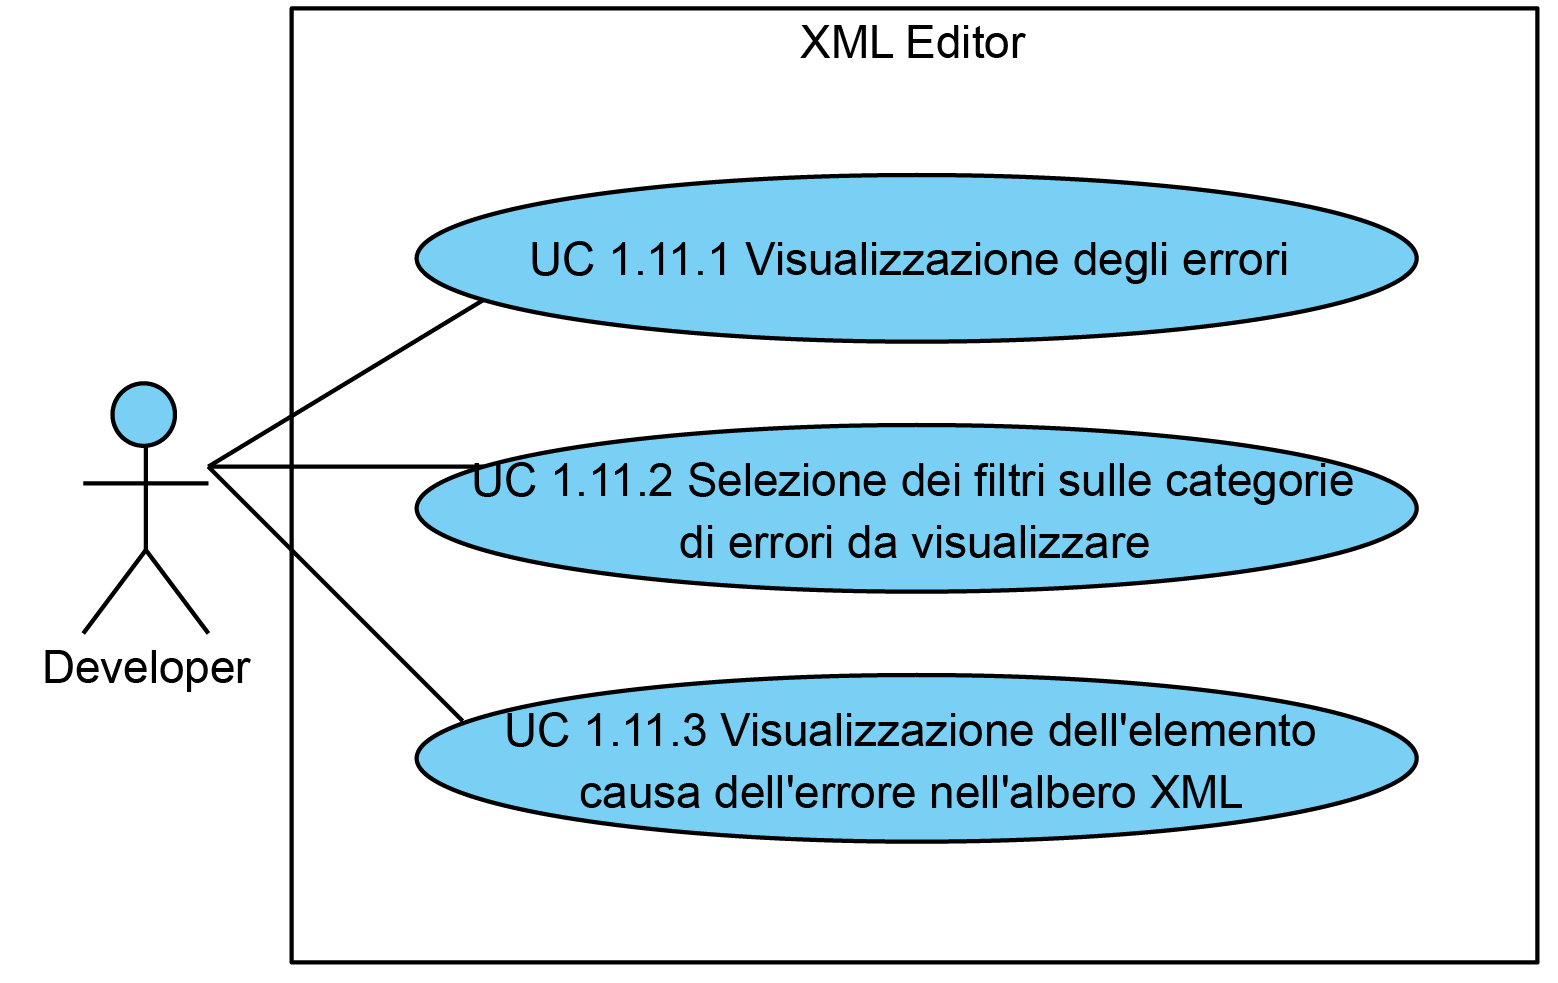
\includegraphics[width=0.9\columnwidth]{tool2/UC1-11.png} 
			\caption{Use Case - UC 1.11 Visualizzazione del risultato del check sulle relazioni}
		\end{figure}
		
		\begin{itemize}
			\item\textbf{Attori}: developer.
			\item\textbf{Descrizione}: un developer deve visualizzare l'esito del check sulle relazioni.
			\item\textbf{Precondizione}: il developer ha avviato il check sulle relazioni e quest'ultimo è terminato.
			\item\textbf{Flusso principale degli eventi}: 
			\begin{enumerate}
				\item \textit{l'utente ha la possibilità di:} \textit{visualizzazione degli errori} (\hyperref[subsec:XEUC1.11.1]{UC 1.11.1});
				
				\item \textit{l'utente ha la possibilità di:} \textit{selezione dei filtri sulle categorie di errori da visualizzare} (\hyperref[subsec:XEUC1.11.2]{UC1.11.2});
				
				\item \textit{l'utente ha la possibilità di:} \textit{visualizzazione dell'elemento causa dell'errore nell'albero XML} (\hyperref[subsec:XEUC1.11.3]{UC1.11.3}).
				
			\end{enumerate}
			\item\textbf{Postcondizione}: il sistema ha permesso la visualizzazione dei risultati del check sulle relazioni.
		\end{itemize}
		
	\subsection{UC 1.11.1 Visualizzazione degli errori}
		\label{subsec:XEUC1.11.1}
		
		\begin{itemize}
			\item\textbf{Attori}: developer.
			\item\textbf{Descrizione}: un developer deve poter l'esito della verifica delle relazioni.
			\item\textbf{Precondizione}: il developer ha avviato il check sulle relazioni e quest'ultimo è terminato.
			\item\textbf{Scenario principale}: viene visualizzato per ogni errore: la severità, la tipologia, la descrizione, il nome del file in cui l'errore è stato trovato.
			\item\textbf{Postcondizione}: il sistema ha visualizzato l'output della verifica delle relazioni.
		\end{itemize}
		
	\subsection{UC 1.11.2 Selezione dei filtri sulle categorie di errori da visualizzare}
		\label{subsec:XEUC1.11.2}
		
		\begin{itemize}
			\item\textbf{Attori}: developer.
			\item\textbf{Descrizione}: un developer deve poter selezionare i filtri sulla severità degli errori.
			\item\textbf{Precondizione}: il developer ha avviato il check sulle relazioni e quest'ultimo è terminato.
			\item\textbf{Scenario principale}: il developer seleziona per ogni categoria di severità se desidera visualizzare gli errori di quella categoria.
			\item\textbf{Postcondizione}: la visualizzazione viene aggiornata e vengono mostrati solo gli errori per il quale corrispettivo filtro di severità è attivo.
		\end{itemize}
		
	\subsection{UC 1.11.3 Visualizzazione dell'elemento causa dell'errore nell'albero XML}
		\label{subsec:XEUC1.11.3}
		
		\begin{itemize}
			\item\textbf{Attori}: developer.
			\item\textbf{Descrizione}: un developer deve poter visualizzare l'elemento causa dell'errore nel suo albero XML di appartenenza.
			\item\textbf{Precondizione}: il developer ha avviato il check sulle relazioni seleziona l'azione per mostrare l'elemento causa dell'errore.
			\item\textbf{Scenario principale}: il developer seleziona l'azione per visualizzare il nodo causa dell'errore nel suo albero di appartenenza.
			\item\textbf{Postcondizione}: il sistema ha visualizzato il nodo nel contesto del suo albero di appartenenza.
		\end{itemize}
		
	\subsection{UC 1.12 Visualizzazione dell'about del programma}
		\label{subsec:XEUC1.12}
		
		\begin{itemize}
			\item\textbf{Attori}: developer.
			\item\textbf{Descrizione}: un developer deve poter visualizzare la finestra about del programma.
			\item\textbf{Precondizione}: il developer abbia selezionato l'azione per visualizzare la finestra about del programma.
			\item\textbf{Scenario principale}: il developer visualizza l'about sul programma.
			\item\textbf{Postcondizione}: il sistema ha mostrato la finestra about del programma.
		\end{itemize}
		
	\subsection{UC 1.13 Visualizzazione degli errori occorsi durante l'apertura del file}
		\label{subsec:XEUC1.13}
		
		\begin{itemize}
			\item\textbf{Descrizione}: si è verificato uno dei seguenti errori durante l'apertura di un file XML:
			\begin{itemize}
				\item il percorso inserito non è valido;
				\item il file indicato non esiste;
				\item il file indicato non è leggibile;
				\item si è verificato un errore non gestito durante l'apertura del file;
				\item il parser XML ha trovato un errore sintattico nel file XML.
			\end{itemize}
			\item\textbf{Precondizione}: il developer ha selezionato l'azione per aprire un file esistente e abbia inserito il percorso ed il nome del file.
			\item\textbf{Scenario principale}: viene fornita una spiegazione dell'errore commesso e come risolverlo.
			\item\textbf{Postcondizione}: l'errore commesso è stato visualizzato e spiegato, il file XML non è stato aperto. Il precedente lavoro è stato chiuso.
		\end{itemize}
		
	\subsection{UC 1.14 Visualizzazione degli errori occorsi durante il salvataggio del file}
		\label{subsec:XEUC1.14}
		
		\begin{itemize}
			\item\textbf{Descrizione}: si è verificato uno dei seguenti errori durante il salvataggio su disco di un file XML:
			\begin{itemize}
				\item il file indicato non è scrivibile;
				\item si è verificato un errore non gestito durante l'apertura in scrittura del file.
			\end{itemize}
			\item\textbf{Precondizione}: il developer ha selezionato l'azione per il salvataggio del file modificato.
			\item\textbf{Scenario principale}: viene fornita una spiegazione dell'errore commesso e come risolverlo.
			\item\textbf{Postcondizione}: l'errore commesso è stato visualizzato e spiegato, il file XML non è stato salvato. Il precedente lavoro non è stato perso.
		\end{itemize}
		
	\subsection{UC 1.15 Visualizzazione degli errori occorsi durante l'importazione}
		\label{subsec:XEUC1.15}
		
		\begin{itemize}
			\item\textbf{Descrizione}: si è verificato uno dei seguenti errori durante l'importazione delle relazioni:
			\begin{itemize}
				\item il percorso inserito non è valido;
				\item il file indicato non esiste;
				\item il file indicato non è leggibile;
				\item si è verificato un errore non gestito durante l'apertura del file;
				\item il parser XML ha trovato un errore sintattico nel file.
			\end{itemize}
			\item\textbf{Precondizione}: il developer ha selezionato l'azione per l'importazione delle relazioni da filee ha inserito un percorso ed il nome del file.
			\item\textbf{Scenario principale}: viene fornita una spiegazione dell'errore commesso e come risolverlo.
			\item\textbf{Postcondizione}: l'errore commesso è stato visualizzato e spiegato, le relazioni non sono state importate. Le precedenti relazioni non sono state eliminate.
		\end{itemize}
		
	\subsection{UC 1.16 Visualizzazione degli errori occorsi durante l'esportazione}
		\label{subsec:XEUC1.16}
		
		\begin{itemize}
			\item\textbf{Descrizione}: si è verificato uno dei seguenti errori durante l'esportazione delle relazioni su un nuovo file:
			\begin{itemize}
				\item il file indicato non è scrivibile;
				\item si è verificato un errore non gestito durante l'apertura in scrittura del file.
			\end{itemize}
			\item\textbf{Precondizione}: il developer ha selezionato l'azione per l'esportazione delle relazioni su file.
			\item\textbf{Scenario principale}: viene fornita una spiegazione dell'errore commesso e come risolverlo.
			\item\textbf{Postcondizione}: l'errore commesso è stato visualizzato e spiegato, le relazioni non sono state esportate.
		\end{itemize}


\section{Tracciamento dei requisiti}
	Partendo dai casi d'uso si è provveduto a stilare una precisa analisi dei requisiti per il tool in questione. I requisiti trovati sono stati inoltre tracciati in relazione al caso d'uso di origine.\\
	
	Di seguito vengono riportati tutti i requisiti individuati. Per essere più leggibili verranno separati in tabelle a seconda della loro categoria. Di ogni requisito verranno indicati: tipologia, importanza e provenienza.\\
	I requisiti dovranno essere classificati per tipo e importanza e utilizzeranno la seguente sintassi:
	\begin{center}
		R[Importanza][Tipo][Codice]
	\end{center}
	\begin{itemize}
		\item \textbf{Importanza}: può assumere solo uno fra i seguenti valori:
		\begin{itemize}
			\item \textit{0}: requisito obbligatorio;
			\item \textit{1}: requisito desiderabile;
			\item \textit{2}: requisito opzionale.
		\end{itemize}
		\item \textbf{Tipo}: pu\`{o} assumere solo uno fra i seguenti valori:
		\begin{itemize}
			\item  \textit{F}: funzionale;
			\item  \textit{Q}: di qualità;
			\item  \textit{P}: prestazionale;
			\item  \textit{V}: vincolo.
		\end{itemize}
		\item \textbf{Codice}: è il codice gerarchico univoco di ogni vincolo espresso in numeri (esempio: 1.3.2).
	\end{itemize}

	Per ogni requisito vengono inoltre specificati:
	\begin{itemize}
		\item \textbf{descrizione}: breve ma completa ed il \underline{meno} ambigua possibile;
		\item \textbf{fonte}: pu\`{o} essere soltanto una o pi\`{u} tra le seguenti:
		\begin{itemize}
			\item \textit{caso d'uso}: il requisito \`{e} stato estrapolato da un caso d'uso. In questo caso va indicato il codice univoco del caso d'uso. \`{E} possibile indicare come fonte pi\`{u} di un caso d'uso.
			\item \textit{interno}: è stato ritenuto giusto aggiungere questo requisito per completezza.
			\item \textit{tutor aziendale}: il requisito è stato espressamente richiesto dal tutor aziendale.
		\end{itemize}
	\end{itemize}

\subsection{Requisiti funzionali}
\begin{center}
	\begin{longtable}{p{4.2cm}!{\color{white}\vrule width 0.5mm}p{6cm}!{\color{white}\vrule width 0.5mm}p{2.5cm}!{\color{white}\vrule width 0.5mm}}
		\rowcolor{headcolor}\textcolor{white}{\textbf{Requisito}}&\textcolor{white}{\textbf{Descrizione}}&\textcolor{white}{\textbf{Fonti}}\\
		
		\rowcolor{row1}\hspace{0mm}\hypertarget{XER0F1}{R0F1} & Un utente può creare un nuovo file XML. & \hyperref[subsec:XEUC1.1]{UC 1.1}\\
		
			\rowcolor{row2}\hspace{2mm}\hypertarget{XER0F1.1}{R0F1.1} & La creazione di un nuovo file XML richiede l'inserimento del percorso dove memorizzarlo. & \hyperref[subsec:XEUC1.1.1]{UC 1.1.1}\\
		
			\rowcolor{row1}\hspace{2mm}\hypertarget{XER0F1.2}{R0F1.2} & La creazione di un nuovo file XML richiede l'inserimento del nome del file. & \hyperref[subsec:XEUC1.1.2]{UC 1.1.2}\\
			
			
			\rowcolor{row2}\hspace{2mm}\hypertarget{XER0F1.3}{R0F1.3} & Se il file inserito è già presente nel sistema, il contenuto verrà sovrascritto solo nel momento del primo salvataggio. & Interno\\
			
		
		\rowcolor{row1}\hspace{0mm}\hypertarget{XER0F2}{R0F2} & Un utente può aprire un file XML preesistente. & \hyperref[subsec:XEUC1.2]{UC 1.2}\\
		
			\rowcolor{row2}\hspace{2mm}\hypertarget{XER0F2.1}{R0F2.1} & L'apertura di file XML richiede l'inserimento del percorso dove recuperarlo. & \hyperref[subsec:XEUC1.2]{UC 1.2}\\
		
			\rowcolor{row1}\hspace{2mm}\hypertarget{R0F2.2}{R0F2.2} & L'apertura di file XML richiede l'inserimento del nome del file da aprire. & \hyperref[subsec:XEUC1.2]{UC 1.2}\\
		
			\rowcolor{row2}\hspace{2mm}\hypertarget{R0F2.3}{R0F2.3} & Se prima dell'apertura di un file XML l'utente ha delle modifiche non salvate su qualche file, il sistema, per ogni file, chiede all'utente se cancellare l'azione, salvare o scartare le modifiche al lavoro precedente. & \hyperref[subsec:XEUC1.2]{UC 1.2}\\
		
	
		\rowcolor{row1}\hspace{0mm}\hypertarget{XER0F3}{R0F3} & Un utente può editare un file XML correntemente aperto e visualizzato. & \hyperref[subsec:XEUC1.3]{UC 1.3}\\
	
			\rowcolor{row2}\hspace{2mm}\hypertarget{XER0F3.1}{R0F3.1} & Un utente può selezionare e visualizzare l'elemento riferito da un elemento. & \hyperref[subsec:XEUC1.3.1]{UC 1.3.1}\\
	
				\rowcolor{row1}\hspace{4mm}\hypertarget{XER0F3.1.1}{R0F3.1.1} & Deve esistere una relazione nel database ed essere istanziata correttamente nell'XML. & Interno\\
	
			\rowcolor{row2}\hspace{2mm}\hypertarget{XER0F3.2}{R0F3.2} & Il programma mostra gli eventuali errori occorsi durante la ricerca del nodo destinazione della relazione. & \hyperref[subsec:XEUC1.3.2]{UC 1.3.2}\\
	
			\rowcolor{row1}\hspace{2mm}\hypertarget{XER0F3.2}{R0F3.2} & Il programma mostra gli eventuali errori occorsi durante la ricerca del nodo destinazione della relazione. & \hyperref[subsec:XEUC1.3.2]{UC 1.3.2}\\
	
			\rowcolor{row2}\hspace{2mm}\hypertarget{XER0F3.3}{R0F3.3} & Un utente può inserire un nuovo nodo figlio ad un elemento. & \hyperref[subsec:XEUC1.3.3]{UC 1.3.3}\\
			
				\rowcolor{row1}\hspace{4mm}\hypertarget{XER0F3.3.1}{R0F3.3.1} & Il programma apre automaticamente la schermata di editing del nuovo nodo inserito. & Tutor interno\\
	
			\rowcolor{row2}\hspace{2mm}\hypertarget{XER0F3.4}{R0F3.4} & Un utente può modificare un nodo dell'albero XML. & \hyperref[subsec:XEUC1.3.4]{UC 1.3.4}\\
			
				\rowcolor{row1}\hspace{4mm}\hypertarget{XER0F3.4.1}{R0F3.4.1} & Un utente può modificare il valore dell'elemento. & \hyperref[subsec:XEUC1.3.4.1]{UC 1.3.4.1}\\
	
				\rowcolor{row2}\hspace{4mm}\hypertarget{XER0F3.4.2}{R0F3.4.2} & Un utente può appendere un nuovo attributo all'elemento. & \hyperref[subsec:XEUC1.3.4.2]{UC 1.3.4.2}\\
	
				\rowcolor{row1}\hspace{4mm}\hypertarget{XER0F3.4.3}{R0F3.4.3} & Un utente può modificare un attributo esistente. & \hyperref[subsec:XEUC1.3.4.3]{UC 1.3.4.3}\\
	
				\rowcolor{row2}\hspace{4mm}\hypertarget{XER0F3.4.4}{R0F3.4.4} & Un utente può rimuovere un attributo esistente. & \hyperref[subsec:XEUC1.3.4.4]{UC 1.3.4.4}\\
	
				\rowcolor{row1}\hspace{4mm}\hypertarget{XER0F3.4.5}{R0F3.4.5} & Il programma blocca il salvataggio se l'utente ha inserito due attributi con lo stesso nome. & Interno\\
	
			\rowcolor{row2}\hspace{2mm}\hypertarget{XER0F3.5}{R0F3.5} & Un utente può duplicare un nodo, inserendo la copia come fratello del nodo copiato. & \hyperref[subsec:XEUC1.3.5]{UC 1.3.5}\\
	
			\rowcolor{row1}\hspace{2mm}\hypertarget{XER0F3.6}{R0F3.6} & Un utente può copiare un nodo e mantenerlo in memoria per essere incollato in un momento successivo. & \hyperref[subsec:XEUC1.3.6]{UC 1.3.6}\\
				
				\rowcolor{row2}\hspace{4mm}\hypertarget{XER0F3.6.1}{R0F3.6.1} & Il programma mantiene un solo nodo copiato alla volta. & Interno\\
	
				\rowcolor{row1}\hspace{4mm}\hypertarget{XER0F3.6.2}{R0F3.6.2} & Ogni nuovo nodo copiato sostituisce quelli precedenti. & Interno\\
	
				\rowcolor{row2}\hspace{4mm}\hypertarget{XER0F3.6.3}{R0F3.6.3} & Se il nodo origine della copia e viene modificato, la copia rimane immutata. & Interno\\
	
			\rowcolor{row1}\hspace{2mm}\hypertarget{XER0F3.7}{R0F3.7} & Un utente può incollare il nodo precedentemente copiato. & \hyperref[subsec:XEUC1.3.7]{UC 1.3.7}\\
	
			\rowcolor{row2}\hspace{2mm}\hypertarget{XER0F3.8}{R0F3.8} & Un utente può rimuovere un nodo. & \hyperref[subsec:XEUC1.3.8]{UC 1.3.8}\\
				
				\rowcolor{row1}\hspace{4mm}\hypertarget{XER0F3.8}{R0F3.8} & Quando il programma rimuove un nodo, vengono rimossi anche tutti i nodi discendenti. & Interno\\
	
			\rowcolor{row2}\hspace{2mm}\hypertarget{XER0F3.9}{R0F3.9} & Un utente può rimuovere tutti i discendenti di un nodo. & \hyperref[subsec:XEUC1.3.9]{UC 1.3.9}\\
			
			\rowcolor{row1}\hspace{2mm}\hypertarget{XER0F3.10}{R0F3.10} & Un utente può istanziare un nuova relazione in automatico, senza dover creare manualmente gli elementi necessari. & \hyperref[subsec:XEUC1.3.10]{UC 1.3.10}\\
			
				\rowcolor{row2}\hspace{4mm}\hypertarget{XER0F3.10.1}{R0F3.10.1} & Affinché l'operazione avvenga con successo è necessario che sia presente un percorso di relazioni che consente di effettuare l'operazione. & Interno\\
	
				\rowcolor{row1}\hspace{4mm}\hypertarget{XER0F3.10.2}{R0F3.10.2} & Se il percorso di relazioni contiene più di un elemento, allora il programma creerà dei nodi intermedi per completare l'operazione. & Interno\\
	
			\rowcolor{row2}\hspace{2mm}\hypertarget{XER0F3.11}{R0F3.11} & Il programma mostra gli eventuali errori occorsi durante l'istanziazione automatica di una relazione. & \hyperref[subsec:XEUC1.3.11]{UC 1.3.11}\\
	
	
			\rowcolor{row1}\hspace{2mm}\hypertarget{XER0F3.12}{R0F3.12} & Un utente può annullare l'ultima modifica effettuata. & \hyperref[subsec:XEUC1.3.12]{UC 1.3.12}\\
			
			\rowcolor{row2}\hspace{2mm}\hypertarget{XER0F3.13}{R0F3.13} & Un utente può ripristinare l'ultima modifica annullata. & \hyperref[subsec:XEUC1.3.13]{UC 1.3.13}\\
	
	
	
			\rowcolor{row1}\hspace{2mm}\hypertarget{R0F3.14}{R0F3.14} & Quando viene effettuata una modifica ad un file XML, viene aggiunto il carattere \sq{*} alla fine del nome per indicare all'utente il nuovo stato del file. & Interno\\
		
		
		\rowcolor{row2}\hspace{0mm}\hypertarget{XER0F4}{R0F4} & Un utente può salvare le modifiche effettuata ad un file XML. & \hyperref[subsec:XEUC1.4]{UC 1.4}\\
		
			\rowcolor{row1}\hspace{0mm}\hypertarget{XER0F4.1}{R0F4.1} & Il programma permette di salvare solo un file su cui sono state apportate modifiche. & \hyperref[subsec:XEUC1.4]{UC 1.4}\\
		
		\rowcolor{row2}\hspace{0mm}\hypertarget{XER0F5}{R0F5} & Un utente può modificare il filtro utilizzato per selezionare l'attributo il cui valore viene mostrato nell'albero per rappresentare l'elemento. & \hyperref[subsec:XEUC1.5]{UC 1.5}\\
			
			\rowcolor{row1}\hspace{0mm}\hypertarget{XER0F5.1}{R0F5.1} & Il valore inserito dall'utente viene memorizzato nel registro di sistema e ripristinato ad ogni apertura del programma. & \hyperref[subsec:XEUC1.5]{UC 1.5}\\
			
		\rowcolor{row2}\hspace{0mm}\hypertarget{XER0F6}{R0F6} & Un utente può modificare i file associati al file correntemente aperto. & \hyperref[subsec:XEUC1.6]{UC 1.6}\\
			
			\rowcolor{row1}\hspace{2mm}\hypertarget{XER0F6.1}{R0F6.1} & Un utente può aggiungere un nuovo file associato. & \hyperref[subsec:XEUC1.6.1]{UC 1.6.1}\\
				
			\rowcolor{row2}\hspace{2mm}\hypertarget{XER0F6.2}{R0F6.2} & Un utente può rimuovere un file associato precedentemente inserito. & \hyperref[subsec:XEUC1.6.2]{UC 1.6.2}\\
		
			\rowcolor{row1}\hspace{2mm}\hypertarget{XER0F6.3}{R0F6.3} & Il programma, in fase di salvataggio delle modifiche applicate ai file associati, non permette il salvataggio se tutti i file associati inseriti non sono tutti differenti fra loro. & \hyperref[subsec:XEUC1.6]{Interno}\\
			
			\rowcolor{row2}\hspace{2mm}\hypertarget{XER0F6.4}{R0F6.4} & Il programma quando salva le modifiche ai file associati, chiude automaticamente quelli rimossi e apre i nuovi inseriti. & Interno\\	
			
		\rowcolor{row1}\hspace{0mm}\hypertarget{XER0F7}{R0F7} & Un utente può editare il database dei tipi di relazioni conosciute dal programma. & \hyperref[subsec:XEUC1.7]{UC 1.7}\\
			
			\rowcolor{row2}\hspace{2mm}\hypertarget{XER0F7.1}{R0F7.1} & Un utente può inserire un nuovo tipo di relazione. & \hyperref[subsec:XEUC1.7.1]{UC 1.7.1}\\
			
				\rowcolor{row1}\hspace{4mm}\hypertarget{XER0F7.1.1}{R0F7.1.1} & L'aggiunta di una nuova relazione richiede l'inserimento del nome del tag origine della relazione. & \hyperref[subsec:XEUC1.7.1]{UC 1.7.1}\\
				
				\rowcolor{row2}\hspace{4mm}\hypertarget{XER0F7.1.2}{R0F7.1.2} & L'aggiunta di una nuova relazione richiede l'inserimento del nome del tag figlio origine della relazione, elemento in cui in un attributo sarà contenuta la chiave dell'elemento destinazione. & \hyperref[subsec:XEUC1.7.1]{UC 1.7.1}\\
					
				\rowcolor{row1}\hspace{4mm}\hypertarget{XER0F7.1.3}{R0F7.1.3} & L'aggiunta di una nuova relazione richiede l'inserimento del nome dell'attributo in è contenuta la chiave dell'elemento destinazione. & \hyperref[subsec:XEUC1.7.1]{UC 1.7.1}\\
					
				\rowcolor{row2}\hspace{4mm}\hypertarget{XER0F7.1.4}{R0F7.1.4} & L'aggiunta di una nuova relazione richiede l'inserimento del nome del tag destinatario della relazione. & \hyperref[subsec:XEUC1.7.1]{UC 1.7.1}\\
						
				\rowcolor{row1}\hspace{4mm}\hypertarget{XER0F7.1.5}{R0F7.1.5} & L'aggiunta di una nuova relazione richiede l'inserimento del nome dell'attributo, nell'elemento destinazione, in cui è presente la chiave identificativa. & \hyperref[subsec:XEUC1.7.1]{UC 1.7.1}\\	
				
			
			\rowcolor{row2}\hspace{2mm}\hypertarget{XER0F7.2}{R0F7.2} & Un utente può modificare tutti i parametri di una relazione precedentemente inserita. & \hyperref[subsec:XEUC1.7.2]{UC 1.7.2}\\
		
			\rowcolor{row1}\hspace{2mm}\hypertarget{XER0F7.3}{R0F7.3} & Un utente può eliminare una relazione precedentemente inserita. & \hyperref[subsec:XEUC1.7.3]{UC 1.7.3}\\
		
			\rowcolor{row2}\hspace{2mm}\hypertarget{XER0F7.4}{R0F7.4} & Il programma salva automaticamente, su file di configurazione XML, le modifiche apportate al database di relazioni. & Tutor interno\\
		
			\rowcolor{row1}\hspace{2mm}\hypertarget{XER0F7.5}{R0F7.5} & Il programma ricarica automaticamente, da file di configurazione XML, il set di relazioni precedentemente presenti nell'ultimo utilizzo del programma. & Tutor interno\\
			
		
		\rowcolor{row2}\hspace{0mm}\hypertarget{XER0F8}{R0F8} & Un utente può importare un set di relazioni presenti in un file di configurazione. & \hyperref[subsec:XEUC1.8]{UC 1.8}\\
		
			\rowcolor{row1}\hspace{2mm}\hypertarget{XER0F8.1}{R0F8.1} & L'importazione richiede che l'utente inserisca il percorso ed il nome del file di configurazione contenente i dati desiderati. & \hyperref[subsec:XEUC1.8]{UC 1.8}\\
			
			\rowcolor{row2}\hspace{2mm}\hypertarget{XER0F8.1}{R0F8.1} & Il programma importa le relazioni contenute, eliminando tutte quelle precedentemente presenti nel database. & Interno\\
		
			\rowcolor{row1}\hspace{2mm}\hypertarget{XER0F8.1}{R0F8.1} & Il programma salva le nuove relazioni nel file di configurazione sostituendo tutte le precedenti. & Interno\\
			
		
		\rowcolor{row2}\hspace{0mm}\hypertarget{XER0F9}{R0F9} & Un utente può esportare tutte le relazione attualmente inserite in un file di configurazione esterno. & \hyperref[subsec:XEUC1.9]{UC 1.9}\\
			\rowcolor{row1}\hspace{2mm}\hypertarget{XER0F9.1}{R0F9.1} & L'esportazione richiede che l'utente inserisca il percorso ed il nome del file di configurazione destinazione. & \hyperref[subsec:XEUC1.9]{UC 1.9}\\
			
				\rowcolor{row2}\hspace{2mm}\hypertarget{XER0F9.1.1}{R0F9.1.1} & Se il file di destinazione non esiste verrà creato. & Interno\\
		
		
		\rowcolor{row1}\hspace{0mm}\hypertarget{XER0F10}{R0F10} & Un utente può avviare il controllo di consistenza delle relazioni sulla base del set di relazioni conosciute dal programma su tutti i file correntemente aperti. & \hyperref[subsec:XEUC1.10]{UC 1.10}\\
			
		\rowcolor{row2}\hspace{0mm}\hypertarget{XER0F11}{R0F11} & Un utente può visualizzare i risultati del controllo di consistenza delle relazioni effettuato sulla base del set di relazioni conosciute dal programma. & \hyperref[subsec:XEUC1.11]{UC 1.11}\\
			
			\rowcolor{row1}\hspace{2mm}\hypertarget{XER0F11.1}{R0F11.1} & Un utente può visualizzare l'elenco degli errori riscontrati durante l'analisi. & \hyperref[subsec:XEUC1.11.1]{UC 1.11.1}\\
			
				\rowcolor{row2}\hspace{4mm}\hypertarget{XER0F11.1.1}{R0F11.1.1} & Il programma mostra per ogni errore la tipologia di questo. & \hyperref[subsec:XEUC1.11.1]{UC 1.11.1}\\
				
				\rowcolor{row1}\hspace{4mm}\hypertarget{XER0F11.1.2}{R0F11.1.2} & Il programma mostra per ogni errore la severità di questo. & \hyperref[subsec:XEUC1.11.1]{UC 1.11.1}\\
				
				\rowcolor{row2}\hspace{4mm}\hypertarget{XER0F11.1.3}{R0F11.1.3} & Il programma mostra per ogni errore una descrizione testuale di questo. & \hyperref[subsec:XEUC1.11.1]{UC 1.11.1}\\
				
				\rowcolor{row1}\hspace{4mm}\hypertarget{XER0F11.1.4}{R0F11.1.4} & Il programma mostra per ogni errore il nome del file nel quale è stato riscontrato. & \hyperref[subsec:XEUC1.11.1]{UC 1.11.1}\\
		
			\rowcolor{row2}\hspace{2mm}\hypertarget{XER0F11.2}{R0F11.2} & Un utente può selezionare un filtro che permette di nascondere o mostrare ogni categoria di errori. & \hyperref[subsec:XEUC1.11.2]{UC 1.11.2}\\
			
			\rowcolor{row1}\hspace{2mm}\hypertarget{XER0F11.3}{R0F11.3} & Un utente può decidere di visualizzare, all'interno dell'albero XML, l'elemento a cui l'errore si riferisce. & \hyperref[subsec:XEUC1.11.3]{UC 1.11.3}\\
		
		
		\rowcolor{row2}\hspace{0mm}\hypertarget{XER0F12}{R0F12} & Un utente può visualizzare la finestra di about sul programma. & \hyperref[subsec:XEUC1.12]{UC 1.12}\\
		
		
		\rowcolor{row1}\hspace{0mm}\hypertarget{XER0F13}{R0F13} & Il programma mostra gli eventuali errori occorsi durante l'apertura di un file XML. & \hyperref[subsec:XEUC1.13]{UC 1.13}\\
		
		\rowcolor{row2}\hspace{0mm}\hypertarget{XER0F14}{R0F14} & Il programma mostra gli eventuali errori occorsi durante il salvataggio di un file XML. & \hyperref[subsec:XEUC1.14]{UC 1.14}\\
		
		\rowcolor{row1}\hspace{0mm}\hypertarget{XER0F15}{R0F15} & Il programma mostra gli eventuali errori occorsi durante l'importazione di un set di relazioni. & \hyperref[subsec:XEUC1.15]{UC 1.15}\\
		
		\rowcolor{row2}\hspace{0mm}\hypertarget{XER0F16}{R0F16} & Il programma mostra gli eventuali errori occorsi durante l'esportazione di un set di relazioni. & \hyperref[subsec:XEUC1.16]{UC 1.16}\\
		
		\hline
		\caption{Requisiti funzionali}
	\end{longtable}
\end{center}

\subsection{Requisiti di qualità}
\begin{center}
	\begin{longtable}{p{4.2cm}!{\color{white}\vrule width 0.5mm}p{6cm}!{\color{white}\vrule width 0.5mm}p{2.5cm}!{\color{white}\vrule width 0.5mm}}
		\rowcolor{headcolor}\textcolor{white}{\textbf{Requisito}}&\textcolor{white}{\textbf{Descrizione}}&\textcolor{white}{\textbf{Fonti}}\\
		
		\rowcolor{row1}\hspace{0mm}\hypertarget{R0Q1}{R0Q1} & Viene fornito insieme al programma un l'help con la guida alla compilazione e al deploy per sistemi Windows. & Tutor interno\\
		
		\hline
		\caption{Requisiti di vincolo}
	\end{longtable}
\end{center}

\subsection{Requisiti di vincolo}
\begin{center}
	\begin{longtable}{p{4.2cm}!{\color{white}\vrule width 0.5mm}p{6cm}!{\color{white}\vrule width 0.5mm}p{2.5cm}!{\color{white}\vrule width 0.5mm}}
		\rowcolor{headcolor}\textcolor{white}{\textbf{Requisito}}&\textcolor{white}{\textbf{Descrizione}}&\textcolor{white}{\textbf{Fonti}}\\
		
		\rowcolor{row1}\hspace{0mm}\hypertarget{R0V1}{R0V1} & Il programma deve funzionare su Windows 7 SP1 32 e 64 bit. & Tutor interno\\
		
		\rowcolor{row2}\hspace{0mm}\hypertarget{R0V2}{R0V2} & Il programma deve essere scritto utilizzando il linguaggio C++ 98. & Tutor interno\\
		
		\hline
		\caption{Requisiti di vincolo}
	\end{longtable}
\end{center}

\section{Tecnologie e strumenti}
Di seguito viene fornita una panoramica delle tecnologie e strumenti utilizzati per lo sviluppo di XML Editor\textsl{}.

	\subsection{Qt\textregistered Framework}
		Per lo sviluppo del tool è stato usato, come per Multiplatform File Analyzer, Qt\textregistered Framework versione 5.3.1.\\
		In particolare è stata usata la libreria per costruire le interfacce grafiche, la libreria per accedere al file system e leggere/scrivere file e la libreria per effettuare il parsing dei file XML.
	
	\subsection{Qt\textregistered Creator}
		Come IDE per lo sviluppo ci si è affidati a Qt\textregistered Creator 3.1.2. IDE semplice e performante che si integra perfettamente con il mondo Qt\textregistered, offrendo addirittura la consultazione veloce della documentazione direttamente nell'IDE.
	
	\section{Ciclo di vita del software}
		XML Editor è stato sviluppato seguendo un modello di ciclo di vita incrementale. È stato deciso di fornire due incrementi. Nel primo sono state inserite tutte le funzionalità per la visualizzazione dei file, la gestione dei file associati e le relazioni (inclusa la verifica). Nel secondo incremento sono state aggiunte alla base già consolidate le funzionalità di editing dei file. Ad ogni incremento è seguito un rilascio del software.

\section{Progettazione}
	Questo software a differenza di Multiplatform File Analyzer, è stato sviluppato secondo il pattern Model-View (todo bibliografica http://qt-project.org/doc/qt-5/model-view-programming.html) ideato dagli ingegneri di Qt\textregistered e sul quale si basa tutto il loro framework. La scelta è stata fatta ragionando sui risultati ottenuti durante lo sviluppo del precedente tool. In esso le esigenze erano diverse, ad esempio la possibilità di poterlo usare da riga comando forzava la scelta verso MVC e il maggior disaccoppiamento possibile dalle classi di Qt\textregistered. Essendo invece questo un editor visuale, che si sarebbe andato a basare proprio sul meccanismo di model-view per gestire ad esempio l'albero XML, si è deciso di sperimentare questo pattern per l'intero sistema. Per lo stagista, questa è la prima volta che si affaccia a questo pattern architetturale ed il suo utilizzo porterà sicuramente una maggior esperienza nella progettazione, permettendogli di valutare pro e contro rispetto al classico MVC.

	La strutturazione generale di alto livello segue quindi il design presentato dal pattern model-view, puntando ad inserire nelle view di competenza le logiche di gestione che, nel mondo MVC, sarebbero appartenute al controller.
	
	I pacchetti in cui il software è stato partizionato sono i seguenti: 
	\begin{itemize}
		\item \texttt{command}: contenente le classi che partecipano all'omonimo design pattern;
		\item\texttt{core}: contenente le classi che implementano il pattern \textit{Strategy} per la realizzazione del controllo sulle relazioni;
		\item\texttt{data}: a cui appartengono le classi di gestione dei dati;
		\item\texttt{observer}: implementazione dell'omonimo design pattern;
		\item\texttt{view}: le classi di visualizzazione del sistema che contengono anche le logiche di controllo.
	\end{itemize}
	
	Per permettere una facile e veloce connessione tra gli strati è stato adottato il Design Pattern \textit{Observer}, implementato nell'omonimo pacchetto \textit{observer}.\\
	
	È stato scelto di utilizzare il Design Pattern \textit{Strategy} per rendere modificabile facilmente l'implementazione dell'algoritmo che effettua l'analisi, all'interno del pacchetto \texttt{core}.\\
	
	A differenza del precedente tool, qui il framework Qt\textregistered è stato usato a tutto tondo ovunque, senza circoscriverne l'uso.

	\subsection{Diagrammi delle classi}
		Vista la vastità del software è stato impossibile creare un diagramma che contenesse contemporaneamente tutte le classi e le relazioni. Sono stati quindi creati due diagramma che permettono di visualizzare due punti importanti dell'architettura. Tutti i diagrammi presenti rispettano il formalismo UML 2.0.
		
		\subsubsection{Data-Model-View diagram}
			In questo diagramma è possibile visualizzare l'integrazione delle classi model-view di Qt\textregistered utilizzate per la visualizzazione dell'albero XML a partire dalla classe di dati. È inoltre presente la logica per il costante aggiornamento della visualizzazione al cambiamento dei dati.
		
		\begin{figure}[!h] 
			\centering 
			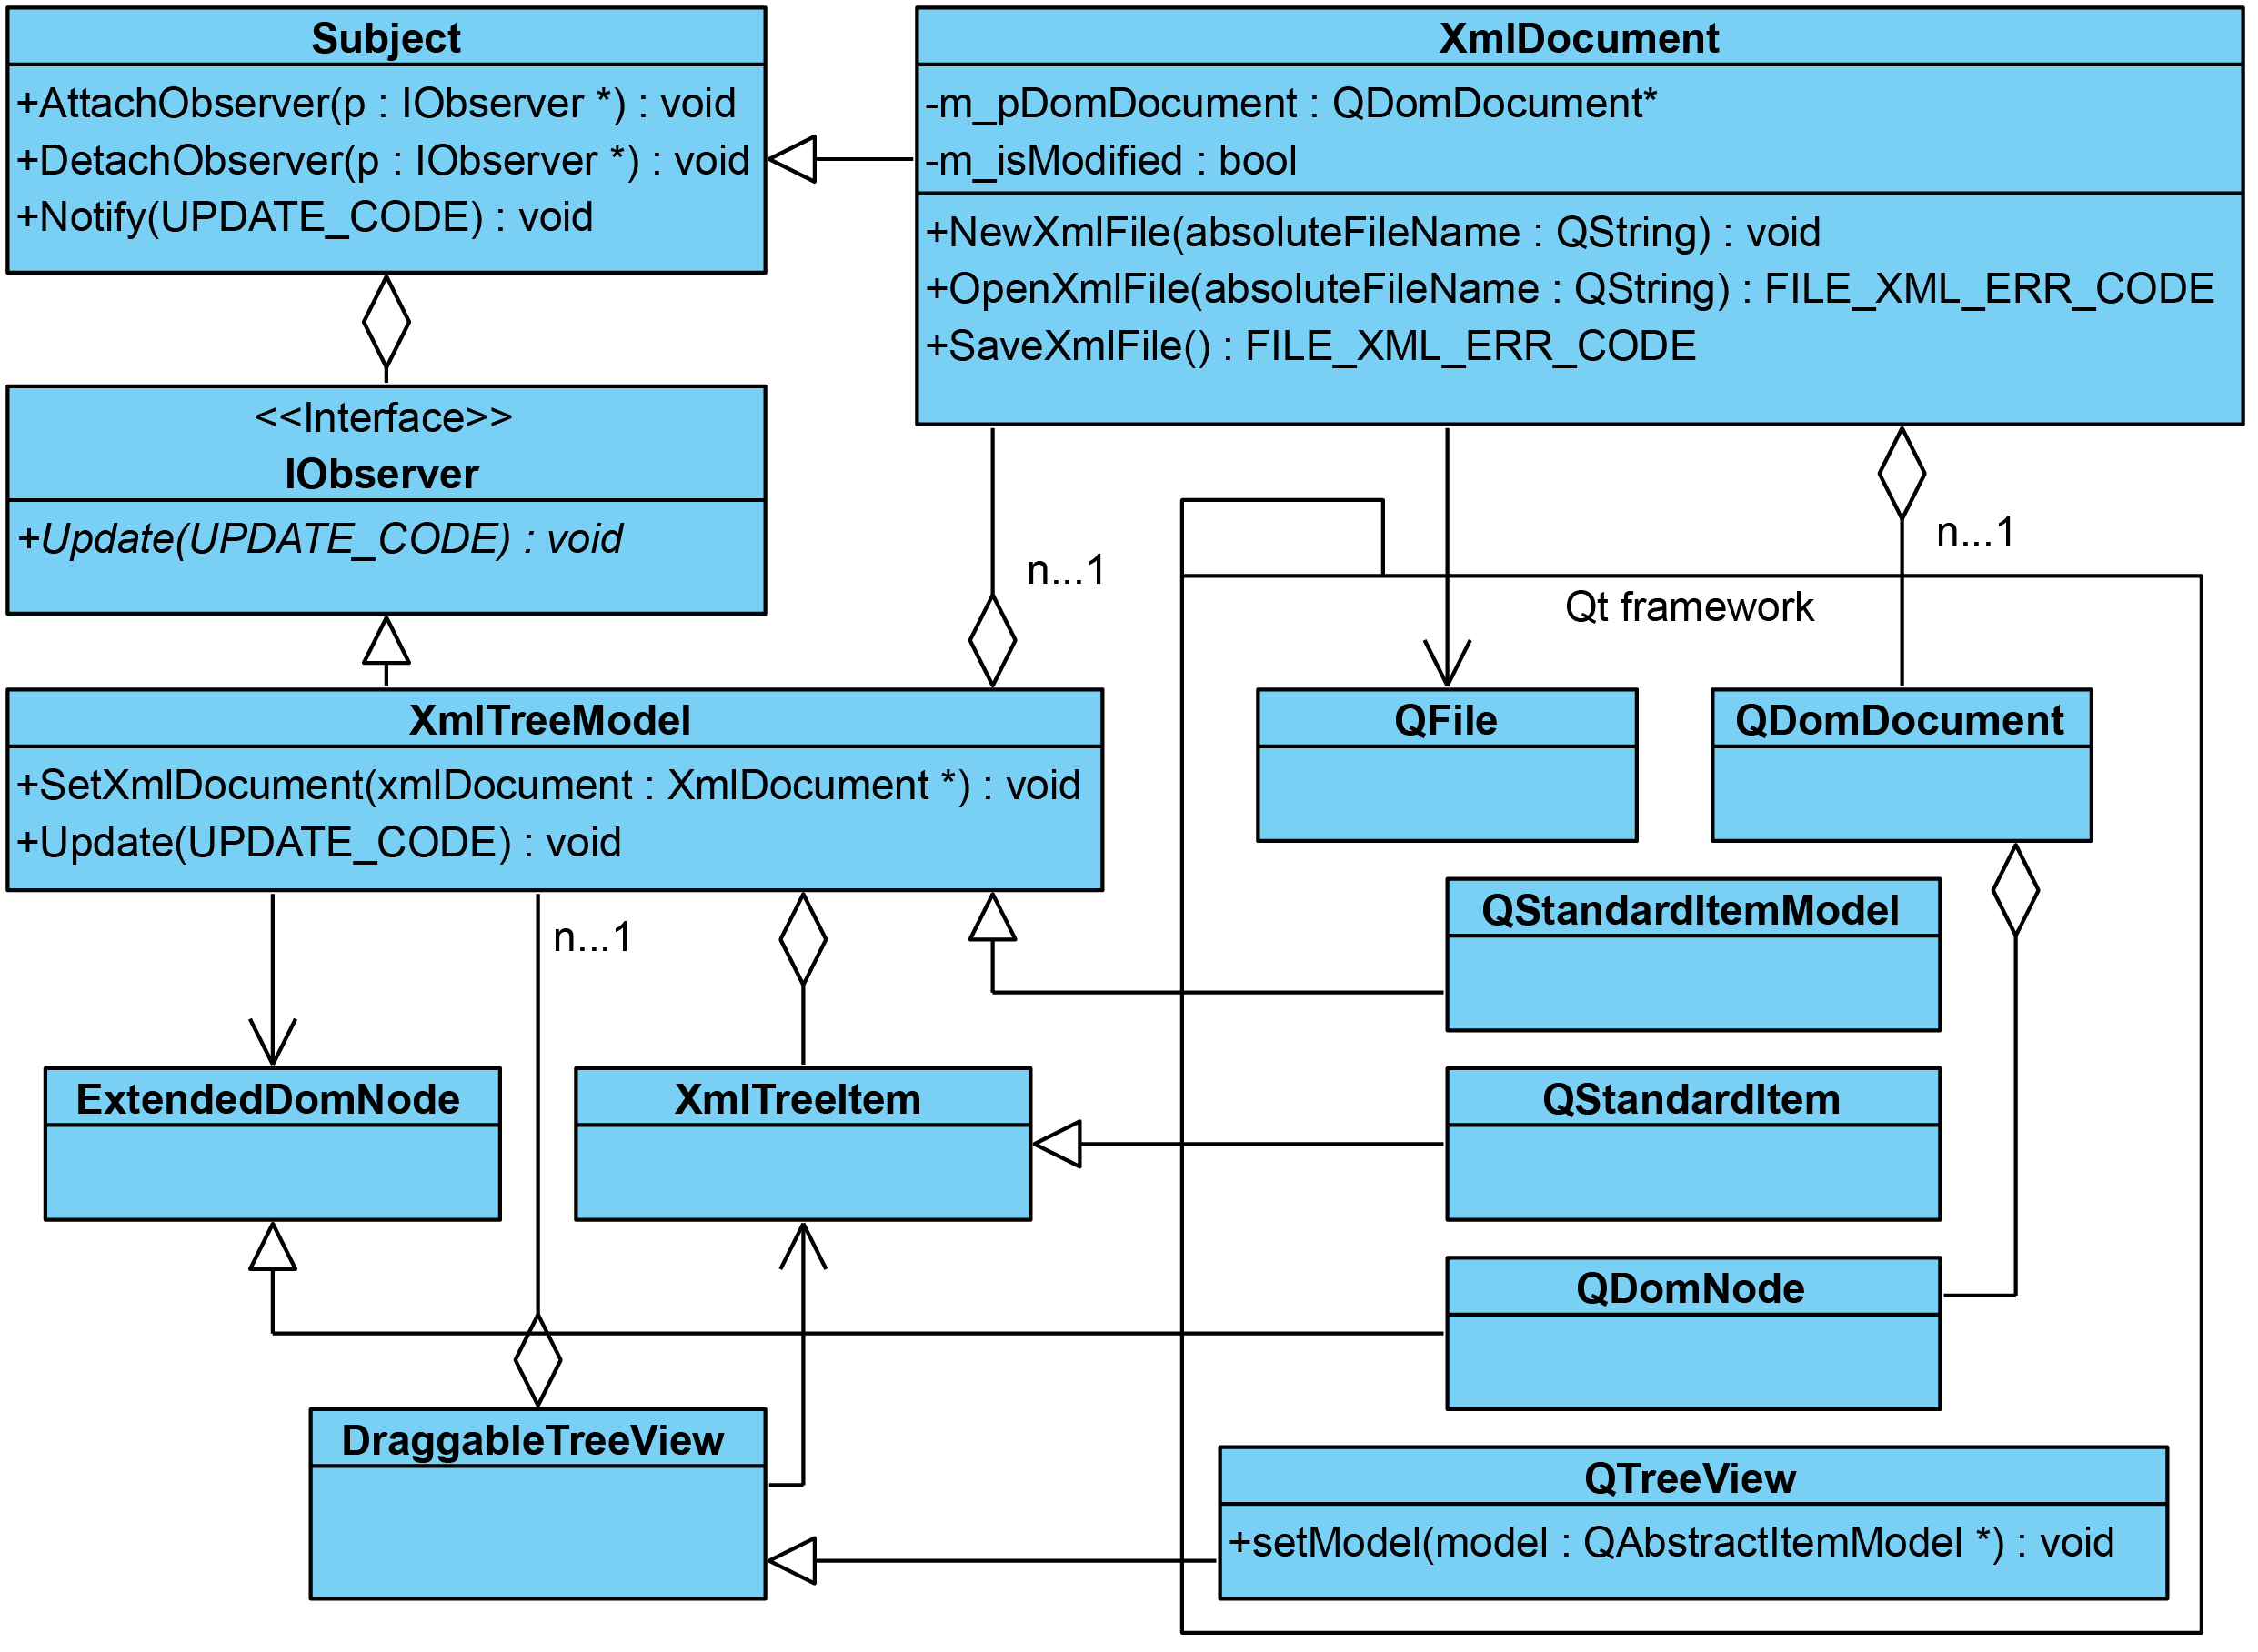
\includegraphics[width=0.98\columnwidth]{tool2/diagramma1.png} 
			\caption{Diagramma dell'integrazione delle classi model-view di Qt\textregistered per la visualizzazione dell'albero XML.}
		\end{figure}
		
		\subsubsection{XML editing diagram}
		In questo diagramma è possibile visualizzare l'implementazione del design pattern \textit{command} usato per gestire l'editing dei file XML. È possibile notare la presenza del design pattern \textit{composite}, inserito allo scopo di permettere la creazione di azioni che si comportassero come singole unità, ma contenessero una aggregazione di azioni base. Un esempio di utilizzo è l'istanziazione automatica di una nuova relazione, la quale crea una singola azione \texttt{XmlEditCommandAggregator} che però esegue tutti i passi intermedi necessari. È a questo punto possibile annullare l'istanziazione con un'unica invocazione del metodo \texttt{Undo} dell'invoker.
		
		\begin{figure}[!h] 
			\centering 
			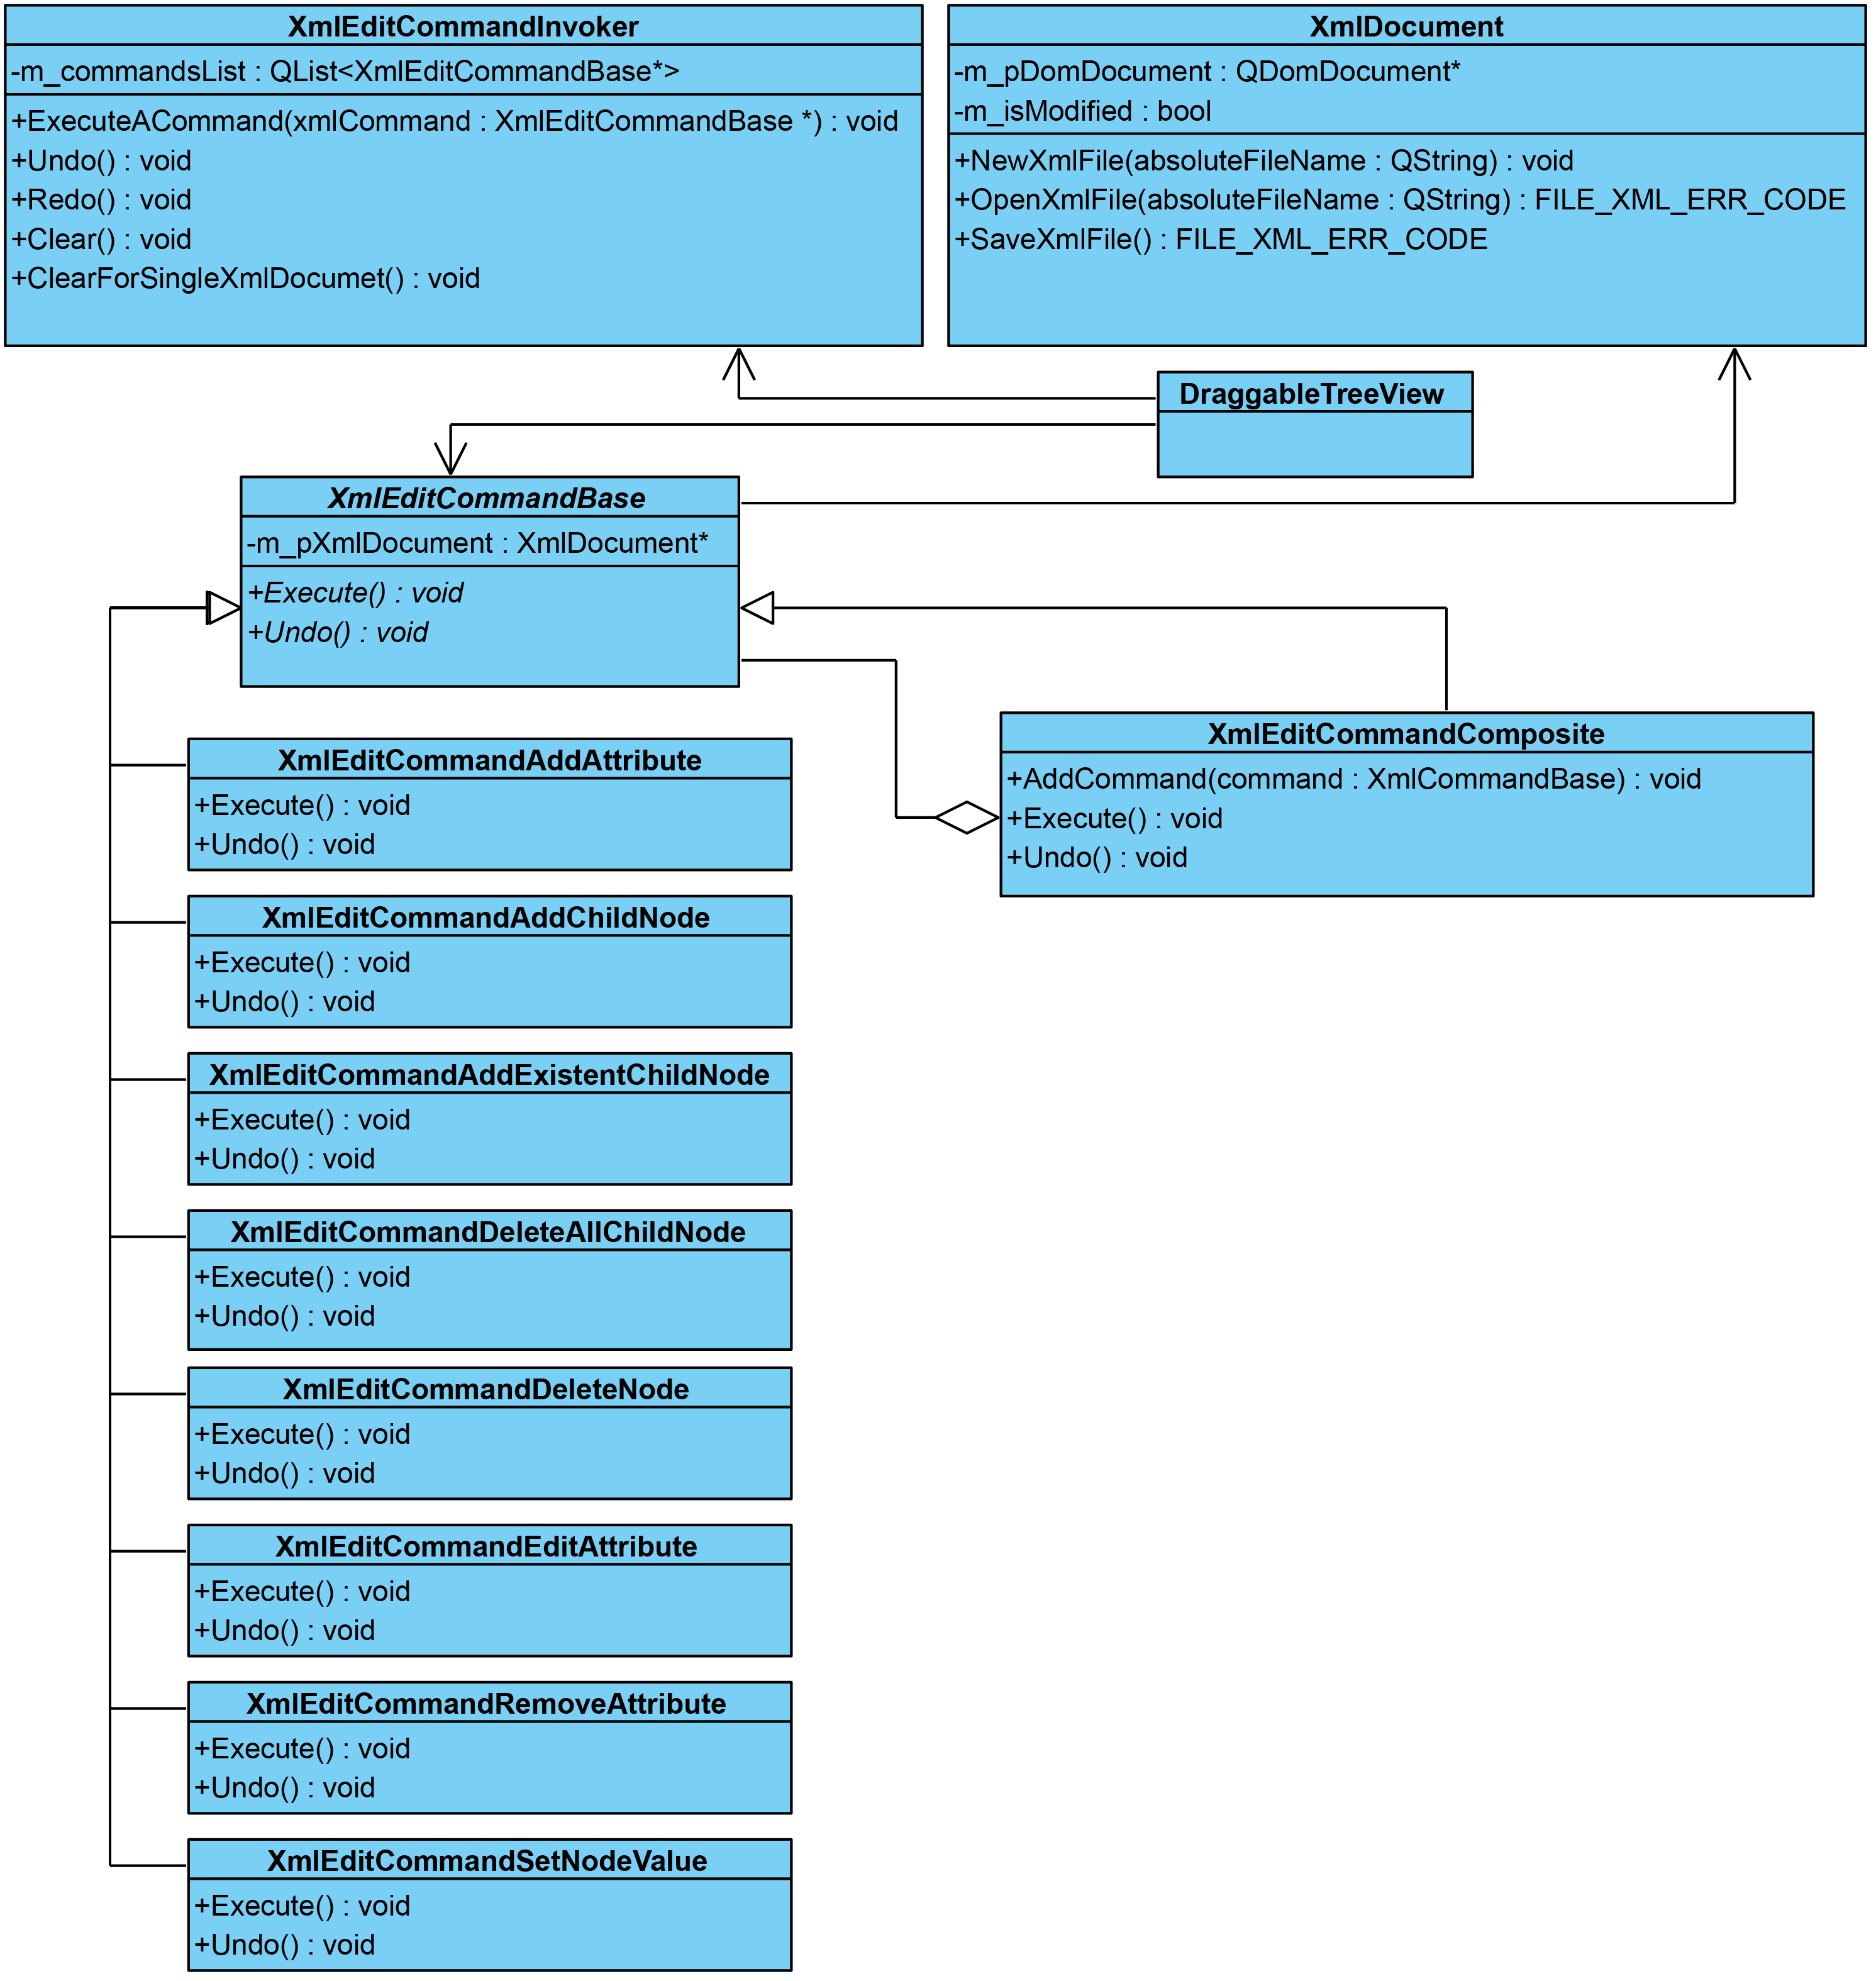
\includegraphics[width=0.98\columnwidth]{tool2/diagramma2.png} 
			\caption{Diagramma delle classi usate per l'editing dei file XML.}
		\end{figure}

\newpage

\subsection{Pacchetto observer}
Questo pacchetto rappresenta l'implementazione del Design Pattern \textit{Observer} ed è stato utilizzato per tenere aggiornata la view al cambiamento dei dati.

	\subsubsection{Interfaccia IObserver}
		\texttt{IObserver} è l'interfaccia che rappresenta gli oggetti che osservano le modifiche di altri oggetti. Essa contiene il metodo virtuale puro \texttt{Update} che i soggetti osservati invocano per segnalare il fatto che sono stati modificati e che quindi un aggiornamento è necessario. Le classi concrete che avranno la necessità di osservare un soggetto deriveranno da \texttt{IObserver} implementando il metodo \texttt{Update}.

	\subsubsection{Classe Subject}
		La classe \texttt{Subject} rappresenta un soggetto che può essere osservato. Essa contiene il codice necessario per notificare tutti gli osservatori dell'avvenuto cambiamento. Mantiene inoltre una lista degli osservatori da notificare, i quali possono iscriversi se desiderano ricevere la notifica, oppure rimuoversi se non è più necessario ricevere aggiornamenti. Le classi che devono essere osservate deriveranno da questa.

\subsection{Pacchetto data}
	Il pacchetto \texttt{data} contiene tutte le classi che rappresentano i dati di business del programma. Come classi aggregazione di base sono state scelte quelle offerte dal framework Qt\textregistered per la loro maggiore integrazione e l'ampio set di funzionalità offerto.

	\subsubsection{Classe AssociatedFiles}
		La classe \texttt{AssociatedFiles} raccoglie tutti i nomi ed i percorsi dei file associati ad un main file. È sua la responsabilità di mantenere la persistenza di queste informazioni tramite la lettura e scrittura nel registro di sistema.
	
	\subsubsection{Classe AttributeNameTagCollapse}
		La classe \texttt{AttributeNameTagCollapse} contiene il filtro sull'attributo da visualizzare nell'albero XML. È sua la responsabilità di mantenere la persistenza di questa informazioni tramite la lettura e scrittura nel registro di sistema.
		
	\subsubsection{Classe XmlDocument}
		La classe \texttt{XmlDocument} rappresenta un file XML aperto nel programma. Ne gestisce la lettura/scrittura su disco e l'effettiva implementazione dell'editing dell'XML.

	\subsubsection{Classe XmlRelation}
		La classe \texttt{XmlRelation} rappresenta un prototipo di relazione, contenendo tutti i dati necessari.
		
	\subsubsection{Classe XmlRelationCollection}
		La classe \texttt{XmlRelationCollection} funge da contenitore per la gestione del set di relazioni cui il programma è a conoscenza.

	\subsubsection{Classe XmlRelationError}
		La classe \texttt{XmlRelationError} rappresenta un errore trovato durante l'analisi di consistenza delle relazioni sulla base dei prototipi conosciuti. Contiene tutte le informazioni dell'errore, le quali saranno mostrate all'utente. È qui presente la logica che compone la stringa descrittiva dell'errore.
		
	\subsubsection{Classe XmlTreeModel}
		La classe \texttt{XmlTreeModel} rappresenta un modello osservabile da una classe view del framework Qt\textregistered. Estende le classi \texttt{QStandardItemModel} e \texttt{Subject}. Essa osserva tramite il pattern \textit{observer} la classe \texttt{XmlDocument} e trasforma il documento XML in un modello visualizzabile dalla classe \texttt{DraggableTreeView}. La classe è un'implementazione del design pattern \textit{Adapter}.
		
	\subsubsection{Classe XmlTreeItem}
		La classe \texttt{XmlTreeItem} estende un classico item del model Qt\textregistered (\texttt{QStandardItem}) inserendo i dati aggiuntivi necessari alla corretta visualizzazione.

\subsection{Core}
	Il pacchetto si occupa della realizzazione dell'analisi e verifica delle relazioni. Utilizza il Design Pattern \textit{Strategy} per l'organizzazione delle classe contenute.

	\subsubsection{Classe XmlRelationCheckerCoreBase}
		\texttt{XmlRelationCheckerCoreBase} rappresenta l'algoritmo di che effettua l'analisi delle relazioni e ritorna una collazione di \texttt{XmlRelationError} con gli errori trovati.
	
	\subsubsection{Classe XmlRelationCheckerCoreImpl}
		La classe \texttt{XmlRelationCheckerCoreImpl} concretizza la base astratta \texttt{XmlRelationCheckerCoreBase} implementando gli algoritmi che effettuano l'analisi dei file verificando la consistenza delle relazioni.

\subsection{Pacchetto command}
Il pacchetto si occupa della gestione delle operazioni di editing dei file XML. Utilizza il Design Pattern \textit{Command} per l'organizzazione delle classe contenute.

	\subsubsection{Classe XmlEditCommandBase}
		\texttt{XmlEditCommandBase} è una classe astratta che rappresenta una operazione eseguibile su un file XML. Mantiene il puntatore al documento XML da editare che verrà usato dalle sottoclassi concrete.
		
	\subsubsection{Classe XmlEditCommandInvoker}
		\texttt{XmlEditCommandInvoker} è la classe che esegue realmente le operazioni mantenendo uno storico di ciò che è stato effettuato offrendo quindi le funzionalità di \texttt{Undo} e \texttt{Redo}

	\subsubsection{Classe XmlEditCommandAggregator}
		\texttt{XmlEditCommandAggregator} è la classe che implementa il design pattern \textit{Command} permettendo l'uso di più comandi come fossero uno singolo.
		
	\subsubsection{Classe XmlEditCommandAddAttribute}
		\texttt{XmlEditCommandAddAttribute} è la classe che implementa il comando di aggiunta di un attributo. Essa mantiene lo stato allo scopo di poter eseguire l'azione di \texttt{Undo}. Per la reale implementazione dell'operazione che essa rappresenta si base sui metodi esposti dalla classe \texttt{XmlDocument}.
		
	\subsubsection{Classe XmlEditCommandAddChildNode}
		\texttt{XmlEditCommandAddChildNode} è la classe che implementa il comando di aggiunta di nuovo nodo vuoto. Essa mantiene lo stato allo scopo di poter eseguire l'azione di \texttt{Undo}. Per la reale implementazione dell'operazione che essa rappresenta si base sui metodi esposti dalla classe \texttt{XmlDocument}.
		
	\subsubsection{Classe XmlEditCommandAddExistentChildNode}
		\texttt{XmlEditCommandAddExistentChildNode} è la classe che implementa il comando di aggiunta di un nodo a partire dalla copia di un nodo precedentemente esistente. Essa mantiene lo stato allo scopo di poter eseguire l'azione di \texttt{Undo}. Per la reale implementazione dell'operazione che essa rappresenta si base sui metodi esposti dalla classe \texttt{XmlDocument}.

	\subsubsection{Classe XmlEditCommandDeleteAllChildNode}
		\texttt{XmlEditCommandDeleteAllChildNode} è la classe che implementa il comando di rimozione di tutti i nodi discendenti di un elemento. Essa mantiene lo stato allo scopo di poter eseguire l'azione di \texttt{Undo}. Per la reale implementazione dell'operazione che essa rappresenta si base sui metodi esposti dalla classe \texttt{XmlDocument}.
			
	\subsubsection{Classe XmlEditCommandDeleteNode}
		\texttt{XmlEditCommandDeleteNode} è la classe che implementa il comando di eliminazione di un attributo e tutti i suoi discendenti. Essa mantiene lo stato allo scopo di poter eseguire l'azione di \texttt{Undo}. Per la reale implementazione dell'operazione che essa rappresenta si base sui metodi esposti dalla classe \texttt{XmlDocument}.
		
	\subsubsection{Classe XmlEditCommandEditAttribute}
		\texttt{XmlEditCommandEditAttribute} è la classe che implementa il comando di editing di un attributo. Essa mantiene lo stato allo scopo di poter eseguire l'azione di \texttt{Undo}. Per la reale implementazione dell'operazione che essa rappresenta si base sui metodi esposti dalla classe \texttt{XmlDocument}.
		
	\subsubsection{Classe XmlEditCommandRemoveAttribute}
		\texttt{XmlEditCommandRemoveAttribute} è la classe che implementa il comando di rimozione di un attributo. Essa mantiene lo stato allo scopo di poter eseguire l'azione di \texttt{Undo}. Per la reale implementazione dell'operazione che essa rappresenta si base sui metodi esposti dalla classe \texttt{XmlDocument}.
		
	\subsubsection{Classe XmlEditCommandSetNodeValue}
		\texttt{XmlEditCommandSetNodeValue} è la classe che implementa il comando di editing del valore di un elemento. Essa mantiene lo stato allo scopo di poter eseguire l'azione di \texttt{Undo}. Per la reale implementazione dell'operazione che essa rappresenta si base sui metodi esposti dalla classe \texttt{XmlDocument}.

\subsection{Pacchetto view}
	Il pacchetto si occupa del display dell'interfaccia utente e della gestione della logica di controllo del software.
	
	\subsubsection{Classe MainWindowView}
		La classe \texttt{MainWindowView} eredita e specializza la classe \texttt{QMainWindow} di Qt\textregistered. Essa è il cuore della logica del programma. Raccoglie e organizza i comandi utente di base, delegando l'esecuzione alle altri componenti del pacchetto.
		
	\subsubsection{Classe DialogAddModifyRelation}
		La classe \texttt{DialogAddModifyRelation} è una dialog creata allo scopo di permettere l'inserimento dei parametri che caratterizzano una relazione da parte dell'utente.
		
	\subsubsection{Classe DialogAssociatedFilesBase}
		La classe \texttt{DialogAssociatedFilesBase} è una base astratta di una finestra di dialog che permette all'utente di gestire i file associati al main file correntemente aperto.
		
	\subsubsection{Classe DialogAssociatedFilesForm}
		La classe \texttt{DialogAssociatedFilesForm} concretizza la base astratta \texttt{DialogAssociatedFilesBase} creando un'interfaccia atta alla gestione dei file associati.
		
	\subsubsection{Classe DialogEditAttributeNameTagCollapseBase}
		La classe \texttt{DialogEditAttributeNameTagCollapseBase} è una base astratta di una finestra di dialog che permette all'utente di gestire il filtro sull'attributo da visualizzare nell'albero XML.
	
	\subsubsection{Classe DialogEditAttributeNameTagCollapse}
		La classe \texttt{DialogEditAttributeNameTagCollapse} concretizza la base astratta \texttt{DialogEditAttributeNameTagCollapseBase} creando un'interfaccia atta alla modifica del filtro sull'attributo da visualizzare nell'albero XML.

	\subsubsection{Classe DialogEditNodeBase}
		La classe \texttt{DialogEditNodeBase} è una base astratta di una finestra di dialog che permette all'utente di editare un nodo XML.
		
	\subsubsection{Classe DialogEditNodeTable}
		La classe \texttt{DialogEditNodeTable} concretizza la base astratta \texttt{DialogEditNodeBase} creando un'interfaccia atta all'editing del valore del nodo e di tutti i suoi attributi.

	\subsubsection{Classe DialogInputFileNameBase}
		La classe \texttt{DialogInputFileNameBase} è una base astratta di una finestra di dialog che permette all'utente di inserire il percorso ed il nome di un file.
	
	\subsubsection{Classe DialogInputFileNameForm}
		La classe \texttt{DialogInputFileNameForm} concretizza la base astratta \texttt{DialogInputFileNameBase} creando un'interfaccia atta all'inserimento di un percorso ed un nome di file. Offre la possibilità di esplorare il file system per un più agevole inserimento. Questa classe è usata per acquisire il file da dove importare o verso dove esportare le relazioni.

	\subsubsection{Classe DialogInputStringBase}
		La classe \texttt{DialogInputStringBase} è una base astratta di una finestra di dialog che permette all'utente di inserire una stringa.
		
	\subsubsection{Classe DialogInputStringForm}
		La classe \texttt{DialogInputStringForm} concretizza la base astratta \texttt{DialogInputStringBase} creando un'interfaccia atta all'inserimento di una stringa da parte dell'utente.
	
	\subsubsection{Classe DialogXmlRelationManagementBase}
	La classe \texttt{DialogXmlRelationManagementBase} è una base astratta di una finestra di dialog che permette all'utente di gestire il database di relazioni.
	
	\subsubsection{Classe DialogXmlRelationManagementTable}
	La classe \texttt{DialogXmlRelationManagementTable} concretizza la base astratta \texttt{DialogXmlRelationManagementBase} creando un'interfaccia atta alla gestione delle relazioni, visualizzate sotto forma tabellare.

	\subsubsection{Classe ViewXmlRelationErrorsBase}
		La classe \texttt{ViewXmlRelationErrorsBase} è una base astratta di una finestra di dialog che permette all'utente di visualizzare il risultato del controllo di consistenza delle relazioni.
		
	\subsubsection{Classe ViewXmlRelationErrorsTable}
		La classe \texttt{ViewXmlRelationErrorsTable} concretizza la base astratta \texttt{ViewXmlRelationErrorsBase} creando un'interfaccia tabellare per la visualizzazione dei risultati sul check delle relazioni.

	\subsubsection{Classe DraggableTreeView}
		La classe \texttt{DraggableTreeView} deriva dalla classe \texttt{QTreeView} del framework Qt\textregistered. Essa è quindi in grado di visualizzare la classe model \texttt{XmlTreeModel} nella quale abilita il drag \& drop per l'istanziazione automatica. È sua responsabilità l'invocazione dei command tramite l'invoker.
	
	
	\subsubsection{Classe XmlViewBase}
		La classe \texttt{XmlViewBase} è una base astratta di un widget per la visualizzazione di file XML.
	
	\subsubsection{Classe XmlViewTree}
		La classe \texttt{XmlViewTree} concretizza la base astratta \texttt{XmlViewBase} creando un widget che mostra un file XML sotto forma di albero.

\section{Codifica}
Tutto il codice del tool è stato pubblicato sulla piattaforma GitHub\textregistered, accedibile tramite il seguente indirizzo: \url{https://github.com/Mauxx91/XML-Editor}. Tutto il codice è disponibile gratuitamente sotto licenza GNU GPL v3\footnote{Un approfondimento sulla licenza può essere trovato al seguente indirizzo: \url{http://www.gnu.org/copyleft/gpl.html}.}\\

Tutto il codice è stato scritto in lingua inglese, compresi i commenti, dei quali si è cercato di scriverne il più possibile.
La codifica ha seguito alcune convenzioni della famosa notazione Ungherese. Di seguito sono elencati i formalismi utilizzati nel codice:

\begin{itemize}
	\item \textbf{prefissi:}
	\begin{itemize}
		\item \textbf{m}: usato per le variabili membro (esempio: \texttt{m\_keyName});
		\item \textbf{p}: usato per le variabili puntatore (esempio: \texttt{m\_pkeyNameList});
		\item \textbf{o}: usato per le variabili input alla funzione che sono usate come output (esempio: \texttt{o\_foundKeys});
		\item \textbf{I}: usato per le classi interfacce (esempio: \texttt{IObserver}).
	\end{itemize}
	\item \textbf{suffissi:}
	\begin{itemize}
		\item \textbf{Base}: usato per le classi astratte (esempio: \texttt{ResultWidgetBase});
	\end{itemize}
	\item \textbf{capitalizzazione:}
	\begin{itemize}
		\item \textbf{variabili e parametri}: iniziano sempre in minuscolo e usano una lettera minuscola per ogni parola (esempio: \texttt{m\_parentWidget}, \texttt{returnValue});
		\item \textbf{macro ed enum}: completamente in maiuscolo con le diverse parole separate dal carattere \sq{\_} (esempio: \texttt{UPDATE\_CODE});
		\item \textbf{classi, funzioni e metodi}: iniziano sempre in maiuscolo e ogni parola diversa parte in maiuscolo (esempio: \texttt{FileOccurrence});
	\end{itemize}
\end{itemize}

todo -> include del codice o no?

\section{Conclusioni}
Tutti i requisiti sono stati soddisfatti come pianificato ma, il secondo incremento comprendente le funzionalità di editing è stata completata con 10 ore di ritardo sulla pianificazione iniziale. 
la realizzazione di questo tool ha permesso allo studente di conoscere davvero approfonditamente il framework Qt\textregistered ed implementare un tool di buona utilità anche all'esterno dell'azienda. L'utilizzo del nuovo design pattern architetturale model-view si è rivelato davvero adatto allo sviluppo di sistemi di questa tipologia, dimostrandosi una valida alternativa a MVC.
             % Product Prototype
% !TEX encoding = UTF-8
% !TEX TS-program = pdflatex
% !TEX root = ../tesi.tex
% !TEX spellcheck = it-IT

%**************************************************************
\chapter{Funzionalità di disegno di elementi grafici 3D a scopo di debug}
\label{cap:game}
%**************************************************************

Lo studente è stato chiamato ad effettuare un refactor\footnote{Per effettuare refactor sono state seguite le linee guida spiegate in \fullcite{inbook:refactoring-book}.} ed implementare nuove funzionalità di disegno di oggetti 3D in game a scopo di debug. Le modifiche sono state apportate al gioco MotoGP 14, delle quali alcune sono state portate a MXGP HD.\\

Si è reso necessario dapprima un'analisi del codice allo scopo di individuare i flussi di interesse e localizzare le vecchie implementazioni su cui effettuare un refactor e sfruttare come base per l'implementazione delle nuove.\\

\section{Stampa dei livelli di LOD di moto e piloti}

In gioco esistono dei moduli grafici che implementano logiche di gestione degli actor di gioco. In particolare esistono in gioco due moduli che gestiscono il calcolo dei livelli di \gloss{LOD} per le moto ed i piloti. Entrambi i moduli sono istanze della classe \texttt{LodSelectionModule}\\

Gli algoritmi più utilizzati per calcolare i livelli di LOD degli oggetti in una scena 3D sono principalmente due. Il primo e più semplice è quello che calcola semplicemente la distanza fra la camera e l'oggetto 3D e scala i livelli secondo una generica funzione (la quale può cambiare a seconda delle tipologie di oggetti o particolari esigenze). Il secondo metodo invece consiste nel calcolare la quantità di pixel occupati dall'oggetto in relazione alla finestra di disegno. Essendo l'oggetto 3D potenzialmente formato da migliaia di poligoni, il calcolo preciso della superficie occupata richiederebbe molto più tempo di quello guadagnato scalando i livelli di dettaglio, si usa quindi un'approssimazione, ad esempio calcolando la superficie della bounding sphere.\\

Il secondo metodo risulta quasi necessario in giochi racing come MotoGP poiché esistono casi in cui il primo algoritmo fallisce molto più spesso del secondo. Si immagini ad esempio un grosso edificio in lontananza visibile dalla pista. Con il primo metodo, l'oggetto in questione, essendo distante, avrà il minimo livello di dettaglio disponibile anche se, essendo anche molto grande occuperà molto spazio su schermo, risultando sgradevole alla vista.\\

\begin{figure}[h!] 
	\centering 
	\hspace*{-0.05\columnwidth}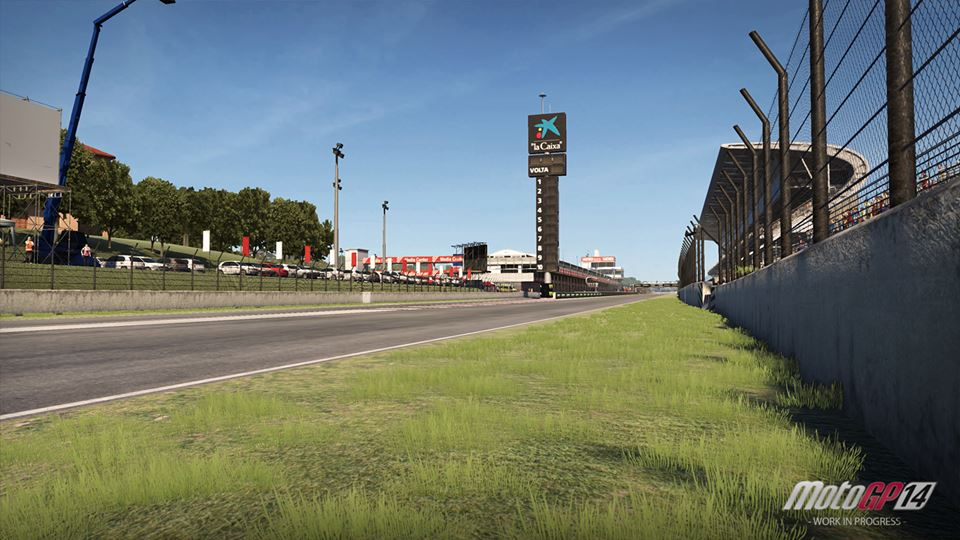
\includegraphics[width=1.1\columnwidth]{game/LODexample.jpg} 
	\caption[Screenshot di MotoGP 14]{Screenshot di MotoGP 14: con il primo metodo la torre sarebbe al lod più basso, invece con il secondo continua ad essere gradevole alla vista}
\end{figure} 

Come già accennato in MotoGP 14 i moduli che gestiscono i livelli di LOD per moto e piloti sono due istanze della classe \texttt{LodSelectionModule}. Essa fornisce, attivabile da Beholder, la funzionalità di stampa dei livelli di LOD correnti degli oggetti per i quali gestisce il livello di dettaglio, in questo caso di moto e piloti presenti al momento in pista. Il problema in questo modulo, era la stampa dei livelli di LOD in posizioni errate, non permettendo di associare il LOD stampato con il suo oggetto. 

\begin{figure}[h!] 
	\centering 
	\hspace*{-0.05\columnwidth}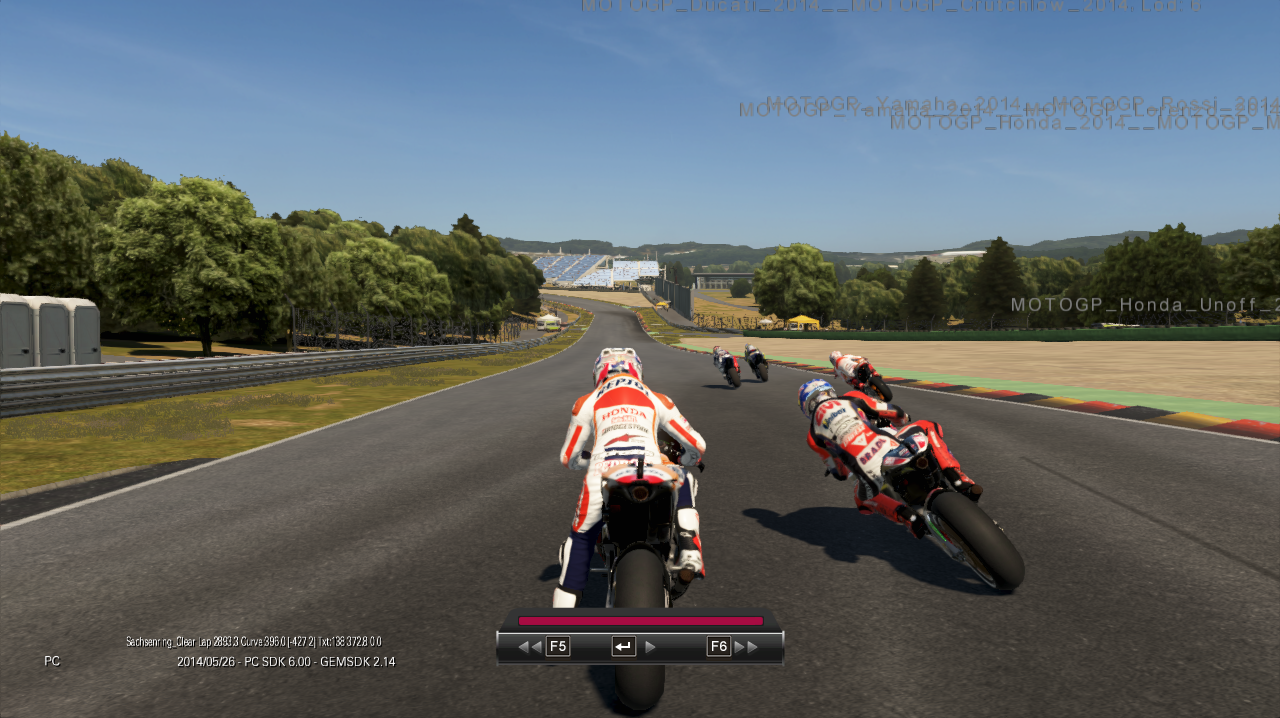
\includegraphics[width=1.1\columnwidth]{game/lodWritesBefore.png}
	\caption{Screenshot di MotoGP 14 nel quale si può osservare la vecchia stampa dei livelli di LOD}
\end{figure}

L'obbiettivo era quindi quello di avere la stampa dell'informazione affiancata all'oggetto, allo scopo di rendere più agevole e veloce il debug e il tuning per ogni piattaforma dell'algoritmo di scelta del LOD.\\

Si parla di tuning dell'algoritmo per ciascuna piattaforma poiché, avendo caratteristiche hardware diverse, le varie piattaforme potranno gestire differenti combinazioni di oggetti con LOD alti. Esiste ad esempio un parametro che indica il massimo numero di bike con LOD 1\footnote{LOD 1 è il massimo livello di dettaglio.}. È compito del team 3D trovare i giusti parametri per permettere il miglior livello grafico possibile per ogni piattaforma.\\ 

Per risolvere il problema è stata inizialmente è stata quindi creata una funzione che trasformasse il punto 3D indicante la posizione dello scene actor, in un punto 2D relativo alle coordinate della finestra di gioco. Punto con il quale si procedeva con la stampa dell'informazione. Viene di seguito riportata la funzione creata.\\

\begin{lstlisting}[style=maurizio-code, caption=Metodo per la trasformazione di un punto 3D in un punto 2D della finestra di gioco rispetto la telecamera corrente, label={code:getScreenPosition}]
void GetScreenPosition(const CCamera* i_pCamera, GVector3& o_position) const
{	
	//Tranform to the homogeneous clip space
	
	//World transformation it's needed
	o_position.TransformPoint(poCamera->GetViewMatrix());
	o_position.TransformPoint(poCamera->GetProjMatrix());
	
	//Now the point is in the range [-1,1] for the x and y axis
	
	//Tranform to the windows space
	o_position.x = (o_position.x + 1) * poCamera->GetViewport().m_uiWidth;
	o_position.y = (o_position.y + 1) * poCamera->GetViewport().m_uiHeight;
	
	//The x cordinate of o_position is simply ignored 
}
\end{lstlisting}
~\\
La funzione \texttt{GetScreenPosition} procede a calcolare le stesse trasformazioni che esegue la GPU per trasformare ogni pixel dell'oggetto nella scena 3D in un'immagine 2D\footnote{Il lettore potrà trovare un approfondimento in \cite[chp.~5]{inbook:directx-book}.}. Si ottengono quindi le coordinate x e y dello schermo nel range [-1, 1]. Si procede quindi a trasformarle in coordinate relative allo spazio dell'intera finestra di gioco (ad esempio 1920x1080px).\\

Con un'analisi più approfondita del codice si è successivamente scoperta la presenza di un metodo della classe \texttt{CCamera} che produceva esattamente gli stessi risultati. Si è quindi provveduto a scartare questa implementazione (seppur corretta) ed usare quella già presente allo scopo di evitare inutili duplicazioni di codice. Di seguito è presente la funzione della classe \texttt{LodSelectionModule} che lancia il disegno del LOD attivo. Questa funzione è lanciata per ogni oggetto gestito dalla classe.\\\vspace*{-0.3cm}

\begin{lstlisting}[style=maurizio-code, caption=Metodo per la stampa del LOD corrente, label={code:printloddebuginformation}]
void LodSelectionModule::PrintLodDebugInformation(CWorld* iWorld, GraphicComponentInfo* i_pComponentInfo )
{
	//Foreach active camera
	for (GUInt camIdx = 0; camIdx < m_pWorld->GetNumberOfCameras(); ++camIdx)
	{
		//Get the string with the lod information and the name of the 3D object
		FixedString256 text;
		i_pComponentInfo->LodToString(camIdx, text);
		
		//Use the old function that calculates the screen point
		GVector2 screenPosition;
		iWorld->GetCurrentCamera(camIdx)->ProjectPoint(i_pComponentInfo->m_pBehavioutInput->GetMatrix().GetTranslation(), screenPosition);
		
		//Draw the LOD information
		DebugTextDrawer::GetInstance()->AppendLog(text.c_str(), screenPosition.x, screenPosition.y);
	}
}
\end{lstlisting}
~\\
Come si può facilmente capire dal codice l'invocazione del metodo \texttt{LodToString} compone la stringa che verrà stampata affianco all'oggetto 3D. Si è modificato tale metodo in modo tale che scrivesse come prima informazione il LOD e poi il nome dello scene actor. Questo perché se l'oggetto è nella parte destra della finestra e ha un nome lungo si corre il rischio che l'informazione più importante (il LOD) finisca fuori dal bordo e non sia visibile.

\begin{figure}[h!] 
	\centering 
	\hspace*{-0.05\columnwidth}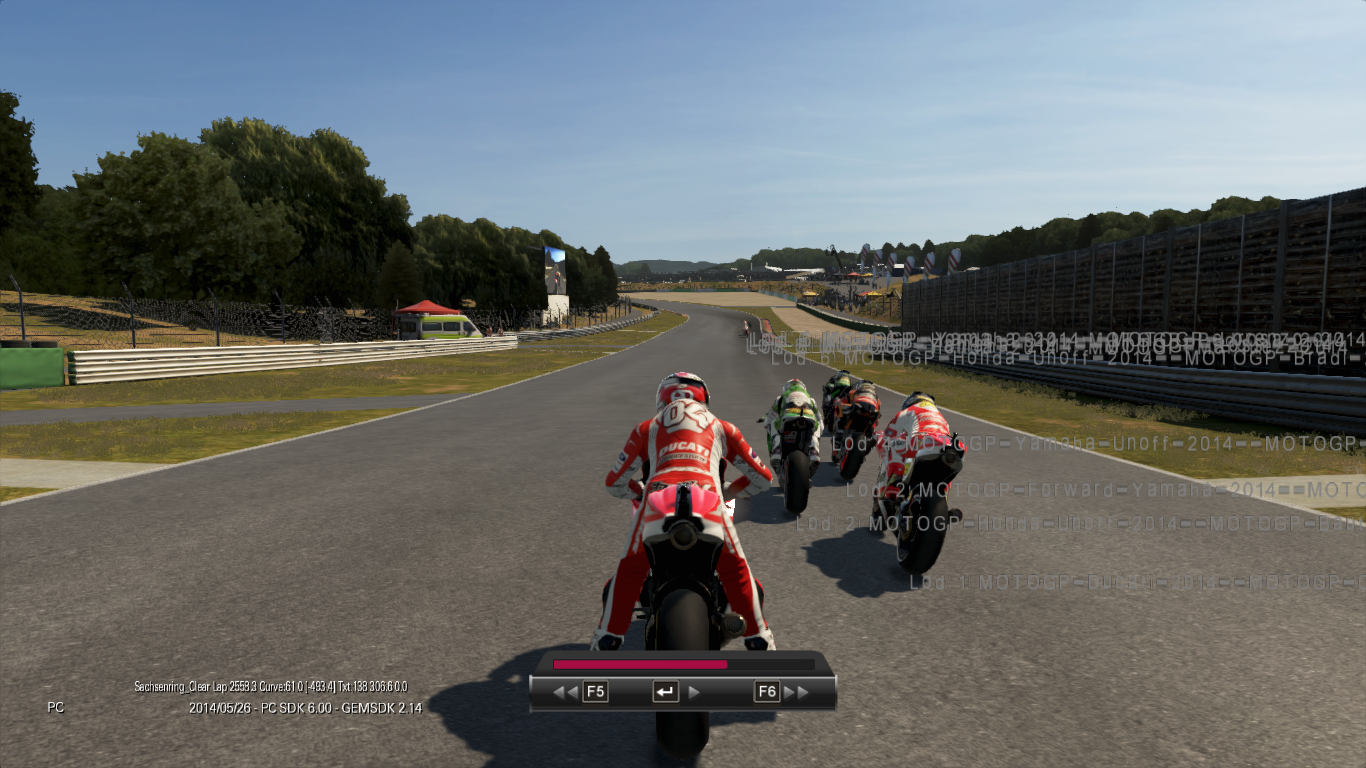
\includegraphics[width=1.1\columnwidth]{game/lodWritesAfterBike.png} 
	\caption{Screenshot di MotoGP 14 nel quale si può osservare la nuova stampa dei livelli di LOD per le moto}
\end{figure}

\begin{figure}[h!] 
	\centering 
	\hspace*{-0.05\columnwidth}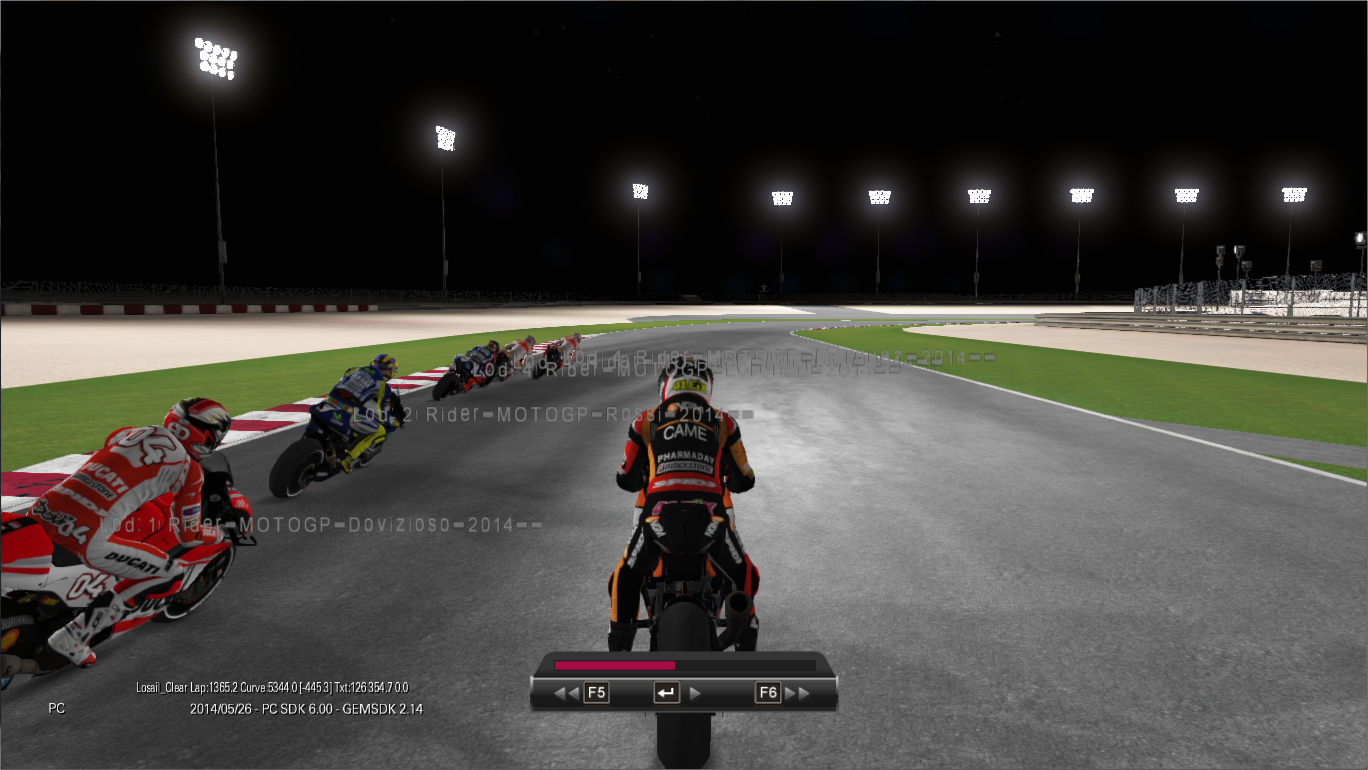
\includegraphics[width=1.1\columnwidth]{game/lodWritesAfterRider.png} 
	\caption{Screenshot di MotoGP 14 nel quale si può osservare la nuova stampa dei livelli di LOD per i piloti}
\end{figure}

Si è poi provveduto ad esporre nel Beholder una variabile membro per ogni istanza della classe \texttt{LodSelectionModule} che permette di attivare e disattivare la stampa di del LOD attivo a run-time.\\

\begin{figure}[h!] 
	\centering 
	\hspace*{-0.05\columnwidth}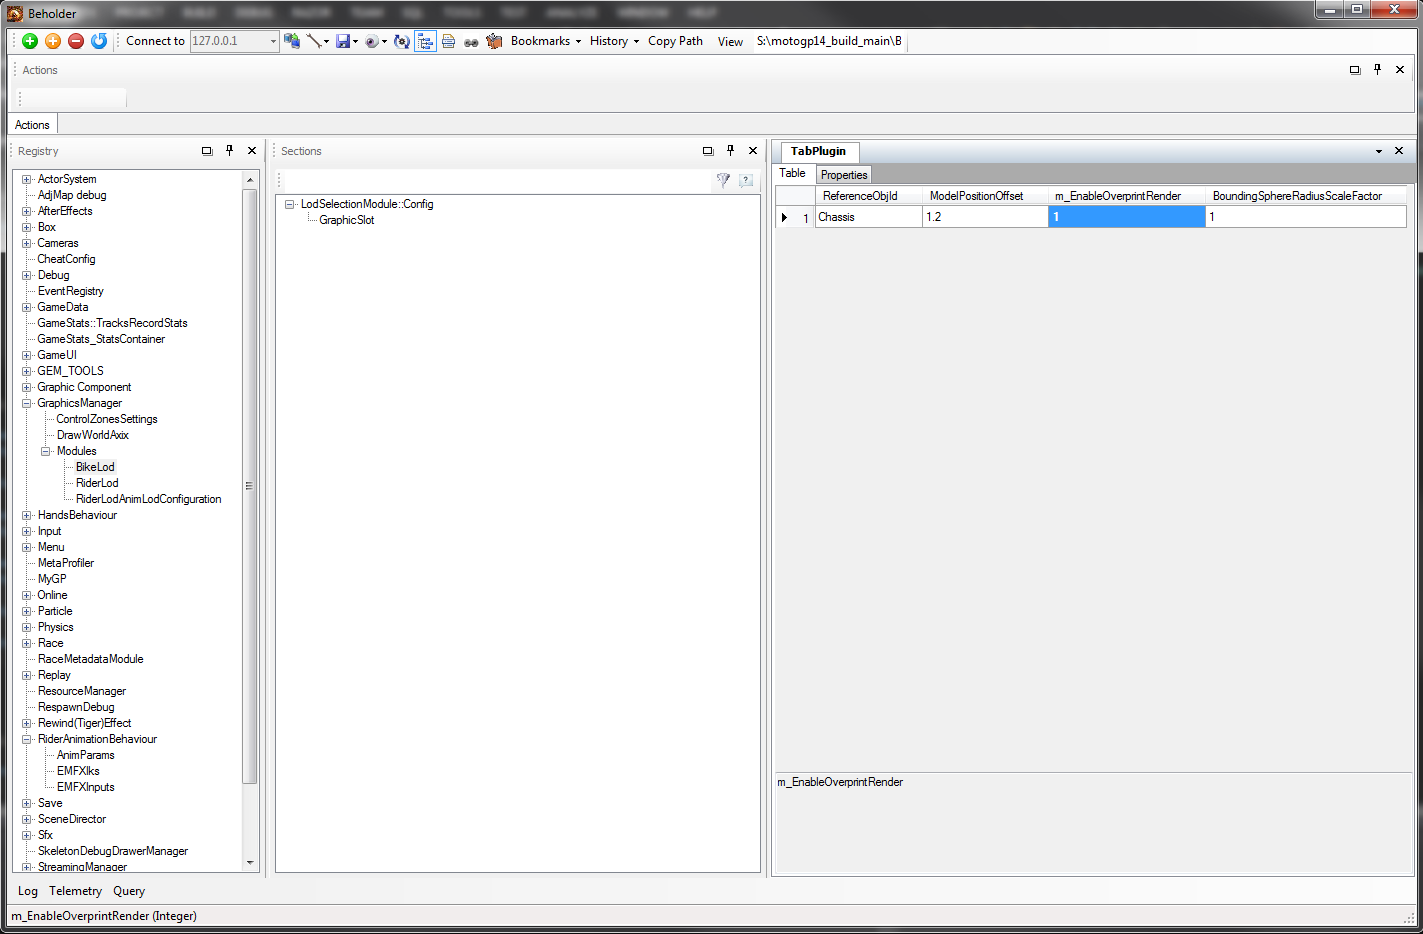
\includegraphics[width=1.1\columnwidth]{game/lodWritesBeholder.png} 
	\caption{Screenshot del Beholder nel quale è possibile vedere dove attivare e disattivare la stampa dei LOD delle moto}
\end{figure}

%\vspace{5cm}

\section{Rifattorizzazione della gerarchia di stampa}

Prestando attenzione al metodo \texttt{PrintLodDebugInformation} presente nel listato \ref{code:printloddebuginformation} si può notare che la stampa a video della stringa è affidata alla classe singleton \texttt{DebugTextDrawer}. Inizialmente la stampa era affidata in gestione alla classe \texttt{LodModule-} \texttt{Debug}, la quale aveva un nome completamente diverso dal compito che svolgeva. Indagando sulle origini di tale classe si è scoperto che questa era stata originata dal \dq{copia e incolla} della classe \texttt{GemScreenLogger}, la quale gestiva la stampa di stringhe in stile terminale, conservando e ristampando le ultime entry inserite e gestendo gli \dq{a capo} e non permettendo sovrapposizioni del testo.\\

Avendo le due classi la maggior parte del codice in comune, si è provveduto ad effettuare un refactor creando una base astratta \texttt{UI\_GemScreenTextBase} dalla quale entrambe derivano e concretizzano implementando i metodi astratti. La classe \texttt{LodModuleDebug} è stata inoltre rinominata in \texttt{DebugTextDrawer} per meglio rispecchiare le sue funzionalità e rendere il codice più comprensibile.\\

\begin{figure}[h!] 
	\centering 
	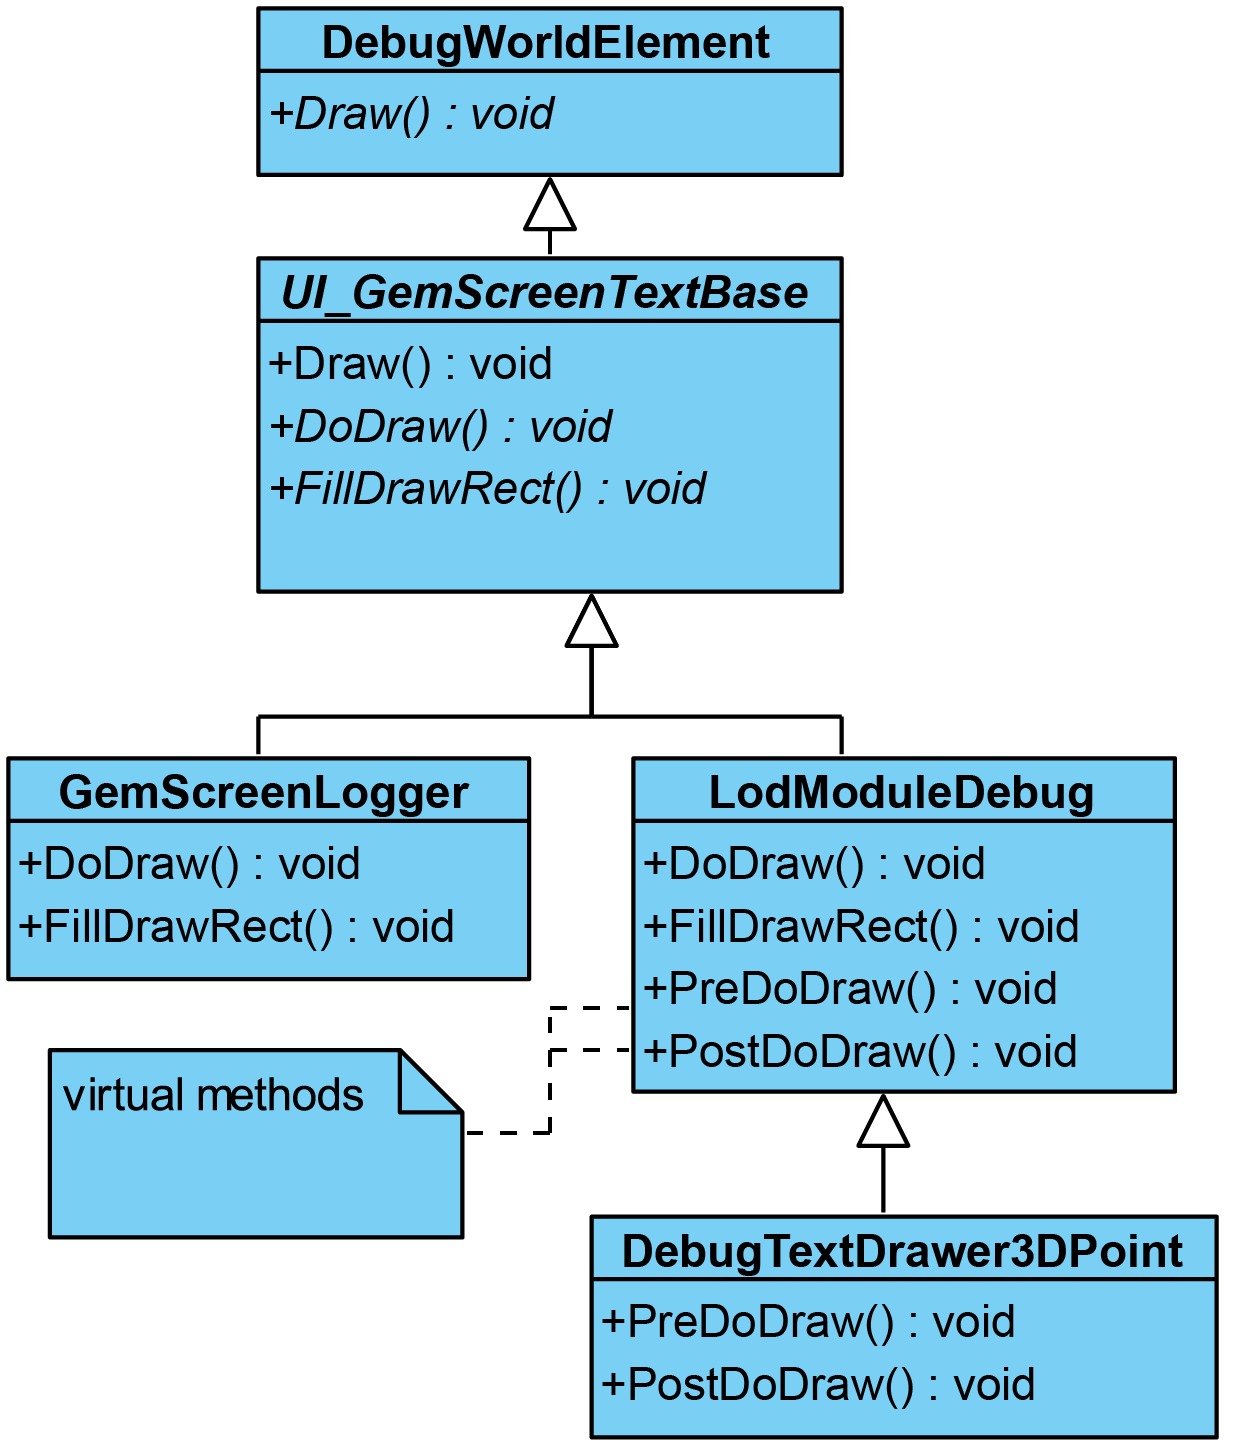
\includegraphics[width=0.6\columnwidth]{game/gerarchiaDrawText.png} 
	\caption{Diagramma UML della gerarchia di stampa del testo. Sono riportati solo i metodi più significativi}
\end{figure}

La classe \texttt{DebugTextDrawer3DPoint} verrà trattata successivamente nella sezione \ref{sec:stampa-del-nome-degli-spazi-di-riferimento}.\\

Le differenze fra le due classi si mostra anche nei loro scenari di utilizzo. \texttt{GemScreen-} \texttt{Logger} accetta dei log e continua a stamparli indipendentemente dai frame. \texttt{DebugText-} \texttt{Drawer} invece, ad ogni frame, stampa tutte le stringhe che possiede e le scarta, non stampandole più al frame successivo. Questo impone quindi che l'inserimento delle scritte sia costante e presente ad ogni frame. Questa caratteristica si adatta perfettamente alla stampa dei LOD, in quanto la posizione su schermo e la stessa informazione varia ad ogni frame e necessita di un costante aggiornamento.\\ 

Come si nota dal diagramma (link diagramma) la gerarchia parte da \texttt{DebugWorld-} \texttt{Element}, classe che rappresenta uno scene actor che può essere inserito in un world. I world sono dei contenitori di oggetti 3D che procedono, se attivi, ad ogni frame a disegnare ogni oggetto presente in essi.\\

Le istanze delle classi concrete della gerarchia vengono, durante la fasi di inizializzazione, inserite nel mondo di debug. Esso è stato creato appositamente per contenere oggetti di debug. Nel resto del gioco, sono presenti implementazioni più specifiche di world, le quali permettono quindi di fare assunzioni sugli oggetti presenti e conseguentemente implementare forti ottimizzazioni. In MotoGP 14 ad esempio sono presenti il \texttt{MenuWorld} ed il \texttt{GameWorld}, che gestiscono rispettivamente il mondo visibile nel menu di gioco ed il mondo visibile durante una gara, permettendone un disegno efficiente.\\

Di seguito è presente la sezione di codice che inizializza gli oggetti della gerarchia in fase di avvio del gioco:

\begin{lstlisting}[style=maurizio-code, caption=Inizializzazione delle classi responsabili della stampa di testo, label={code:initTextClasses}]
GemScreenLogger::Create();
debugWorld->AddElement( UI::GemScreenLogger::GetInstance() );

DebugTextDrawer::Create();
DebugTextDrawer::Config config;
config.m_fontName = "Linotype Univers 430 Regular20";
config.m_alphaValue = 255;
config.m_timeBeforeFade = 500;
config.m_includeContext = false;
config.m_includeSourceFile = false;
config.m_timestamp = false;

DebugTextDrawer::GetInstance()->Init();
DebugTextDrawer::GetInstance()->SetConfig( config );
debugWorld->AddElement( DebugTextDrawer::GetInstance() );

DebugTextDrawer3DPoint::Create();
DebugTextDrawer3DPoint::GetInstance()->Init();
config.m_timeBeforeFade = 9999999999;
DebugTextDrawer3DPoint::GetInstance()->SetConfig( config );
debugWorld->AddElement( DebugTextDrawer3DPoint::GetInstance() );
\end{lstlisting}

\section{Stampa del nome degli spazi di riferimento}
\label{sec:stampa-del-nome-degli-spazi-di-riferimento}

Una funzionalità già presente è la stampa degli assi di riferimento degli oggetti presenti nella scena 3D e dell'asse origine del mondo. L'obbiettivo quindi è stato l'inserimento della stampa del nome dell'oggetto affianco al disegno dell'asse allo scopo di poterli riconoscere fra loro quando se ne disegnano più d'uno. Per realizzare questa funzionalità si è proceduto alla creazione della classe \texttt{DebugTextDrawer3DPoint}. Essa deriva da \texttt{DebugTextDrawer} della quale specializza semplicemente l'inserimento della stringa, allo scopo di poter continuare a disegnare il testo nella corretta posizione (che può cambiare) senza dover chiamare il disegno della stringa ogni frame. Il disegno degli assi è attivato dal Beholder da diversi contesti.\\

\begin{figure}[h!] 
	\centering 
	\hspace*{-0.05\columnwidth}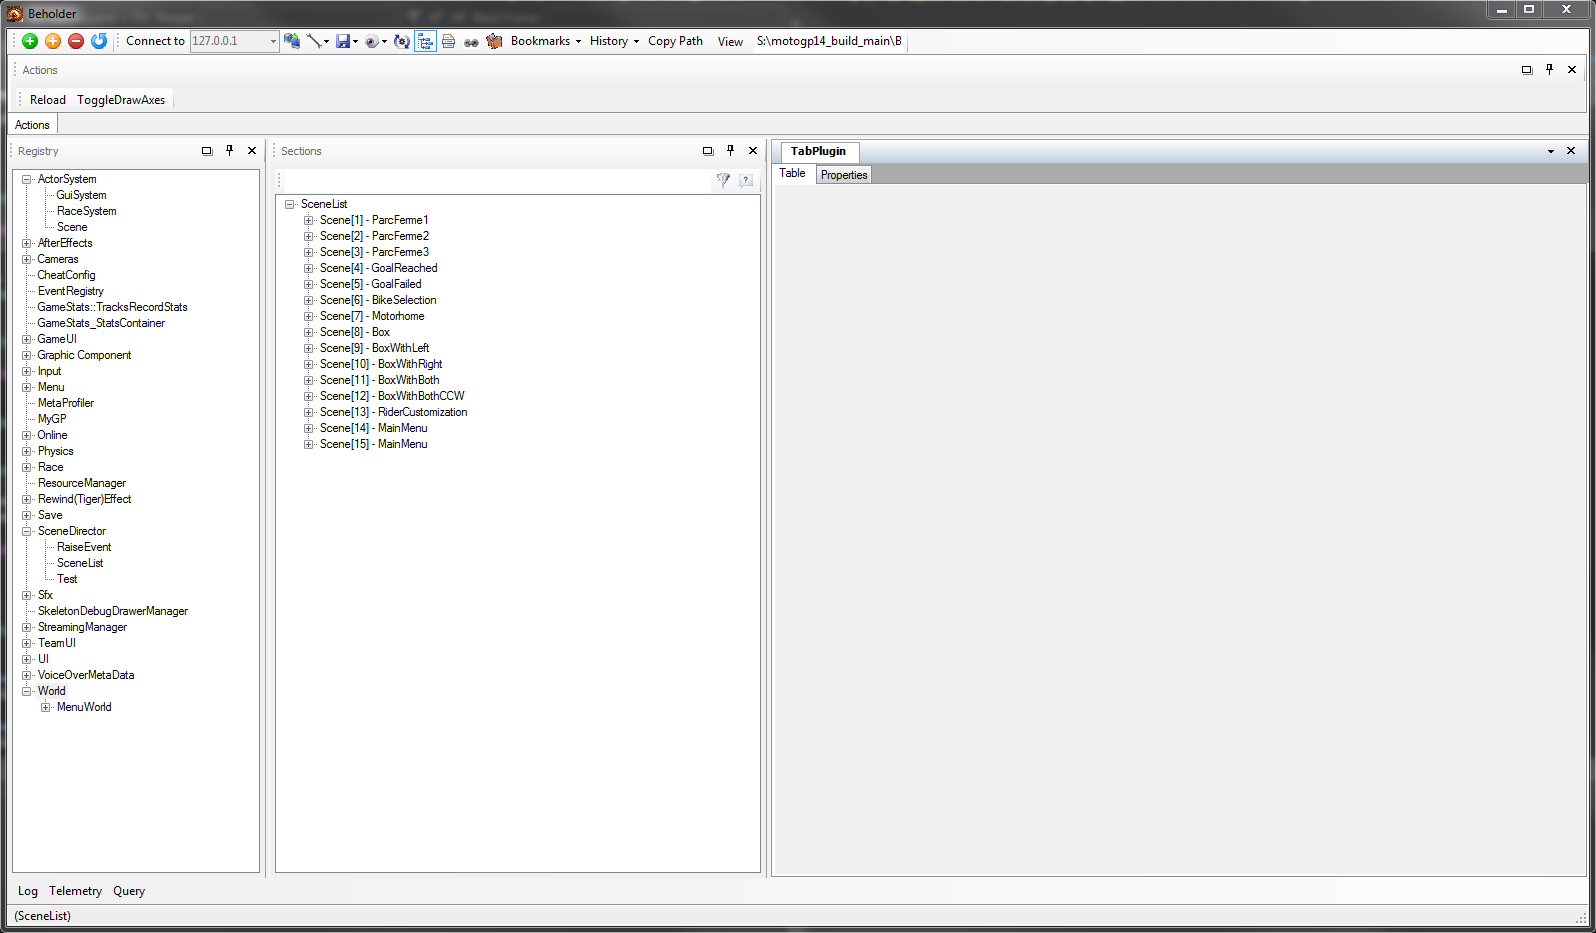
\includegraphics[width=1.1\columnwidth]{game/BeholderDrawSceneAxis.png} 
	\caption{Screenshot del Beholder nel quale è possibile lanciare il disegno degli assi tramite l'azione \dq{ToggleDraeAxes} dello \dq{SceneDirector} visibile in alto a sinistra}
\end{figure}

\texttt{DebugTextDrawer} provvede ad ogni frame, tramite un puntatore alla camera attiva e una reference alla matrice della posizione, che può quindi essere aggiornata, ad effettuare il calcolo del punto 3D a partire dal punto 2D e lanciare la stampa ad ogni frame. L'appesa di un log a questa classe richiede quindi della camera attiva, del testo e della matrice che contiene la posizione 3D. In questo modo è possibile disegnare il nome dell'asse, e continuare a visualizzare il nome ad ogni frame, senza dover appendere il log ad ogni frame come con \texttt{DebugTextDrawer}. Questo si è reso necessario in quanto il submit degli oggetti 3D che rappresentano gli assi avviene una volta soltanto, rendendo quindi necessaria l'utilizzo di un meccanismo simile anche per il testo correlato.

Lo studente ha provveduto quindi a individuare i punti del codice in cui erano presenti le chiamate di disegno degli assi allo scopo di implementare la nuova funzionalità, scoprendo che il codice per disegnarli era duplicato molteplici volte.\\

Si è proceduto quindi ad eseguire un refactor creando una classe specializzata nel disegno di assi con l'etichetta del nome dell'oggetto, la classe \texttt{DebugAxisDrawer}.\\

Essa provvede a incapsulare la funzione che si occupa del disegno degli assi e, eseguendo il codice necessario a ottenere la telecamera attiva, a lanciare la stampa del nome dell'oggetto. Come accennato, la funzionalità di disegno degli assi è lanciata durante un particolare stato in cui le geometrie disegnate, una volta eseguito il submit, vengono renderizzate ogni frame senza doverne richiedere la rappresentazione ad ogni frame. Si procede quindi allo stesso modo per il testo associato grazie alla classe \texttt{DebugTextDrawer3DPoint}.\\

Di seguito si riporta il codice della classe \texttt{DebugAxisDrawer}.

\lstinputlisting[style=maurizio-code, caption=DebugAxisDrawer.h, label={code:DebugAxisDrawer-h}]{code/DebugAxisDrawer.h}

\lstinputlisting[style=maurizio-code, caption=DebugAxisDrawer.cpp, label={code:DebugAxisDrawer-cpp}]{code/DebugAxisDrawer.cpp}

\begin{figure}[h!] 
	\centering 
	\hspace*{-0.05\columnwidth}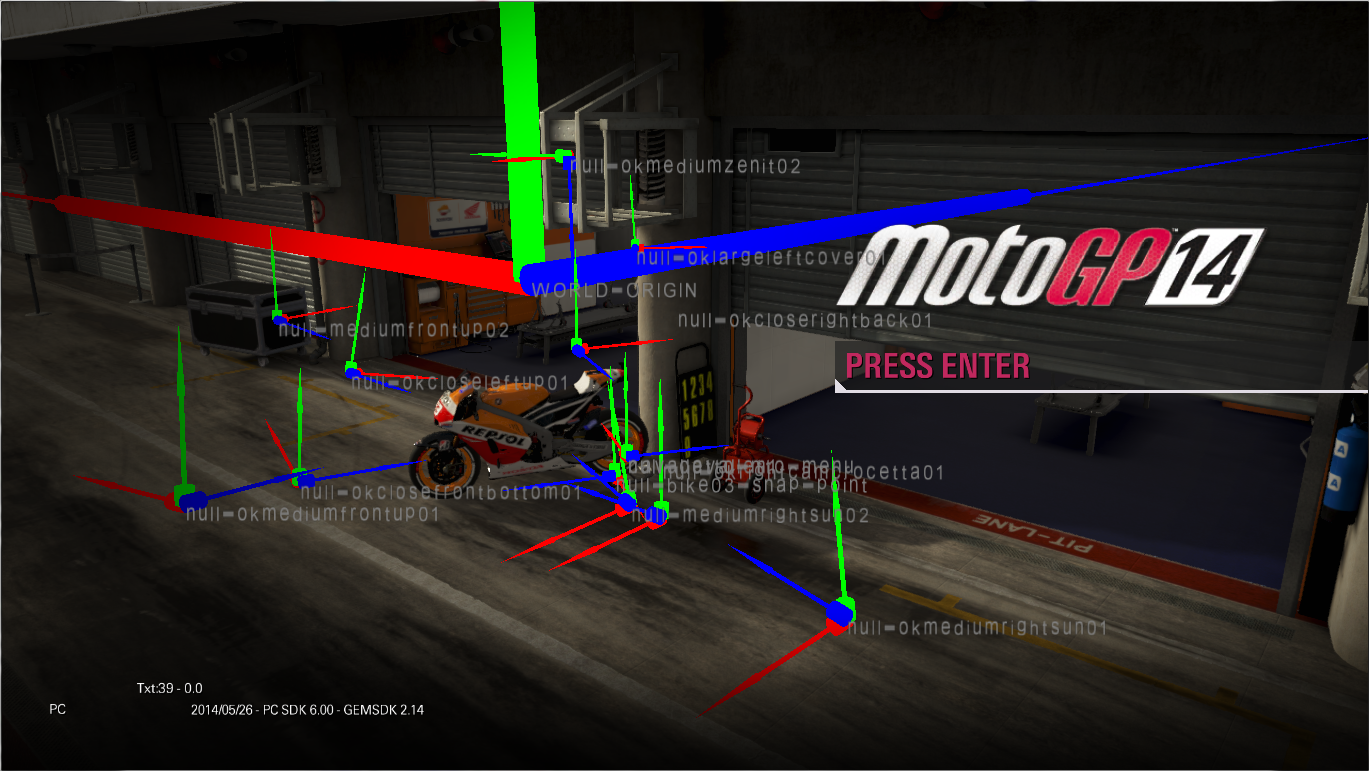
\includegraphics[width=1.1\columnwidth]{game/menuDrawAxisText.png} 
	\caption{Screenshot di MotoGP 14 in cui nel main menu è possibile vedere gli assi dei punti in cui viene ancorata la camera e la stampa del nome corrispondente}
\end{figure}

\section{Vista gerarchica dei world nel Beholder}
	Nel Beholder è possibile visualizzare tutte le risorse grafiche presenti nel \texttt{Resour-} \texttt{cesManager}. Questa classe gestisce il caricamento e lo scaricamento in memoria di tutte le risorse grafiche utilizzate per costruire le scene 3D del gioco. Essa utilizza la strategia di reference couting per sapere quando un oggetto diviene inutilizzato e può essere quindi scaricato. Essa contiene quindi una collezione di world in cui sono presenti le varie risorse (mesh, texture, animazioni, ecc..). Per ogni tipo di risorsa presente nel world nel Beholder viene presentata come lista piatta. È possibile invece che queste risorse siano imparentate fra di loro, formando ad esempio delle gerarchie di oggetti 3D.\\
	
	\begin{figure}[h!] 
		\centering 
		\hspace*{-0.05\columnwidth}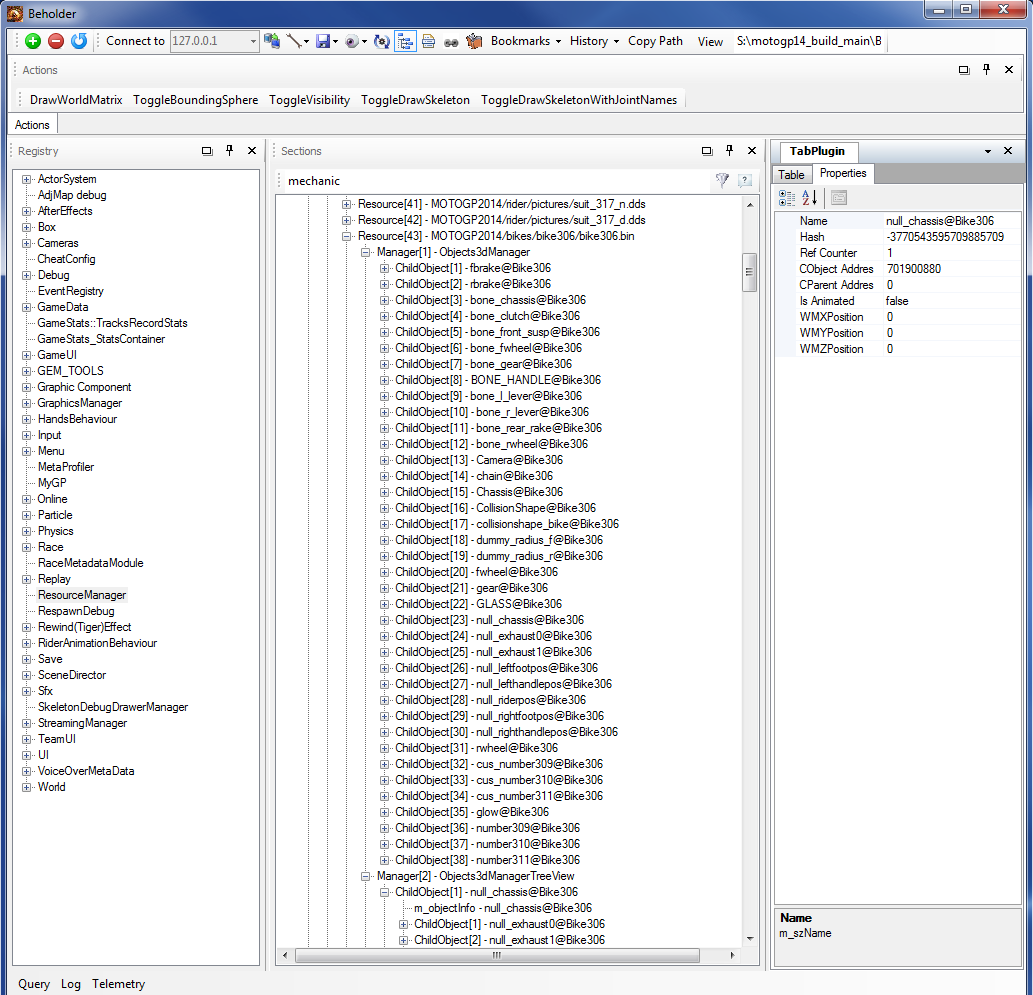
\includegraphics[width=1.1\columnwidth]{game/beholderResourceManagerView.png} 
		\caption{Screenshot del Beholder in cui è possibile visualizzare la versione a lista piatta sopra e la versione ad albero sotto per la bike 306}
		\label{fig:resource-manager-tree-view}
	\end{figure}
	
	Si è proceduto quindi a creare una versione ad albero per la categoria degli Object3D presenti nel world.\\
	
	Il contenuto del \texttt{ResourcesManager} è esposto nel Beholder tramite la classe \texttt{Resources-} \texttt{ManagerDebug} in cui si concentrano le modifiche effettuate per poter offrire la nuova funzionalità.
	
	Di seguito vengono riportati alcune sezioni del codice della classe significative per la nuova funzionalità inserita.
	
	\lstinputlisting[style=maurizio-code, caption=ResourcesManagerDebug.h, label={code:ResourcesManagerDebug-h}]{code/ResourcesManagerDebug_new.h}
	
	\newpage
	
	\lstinputlisting[style=maurizio-code, caption=ResourcesManagerDebug.cpp, label={code:ResourcesManagerDebug-cpp}]{code/ResourcesManagerDebug_new.cpp}
	
	\lstinputlisting[style=maurizio-code, caption=ResourcesManagerDebug\_Metadata.cpp, label={code:ResourcesManagerDebug-Metadata-cpp}]{code/ResourcesManagerDebug_newMetadata.cpp}

\section{Disegno degli scheletri di animazione}
	
	Allo scopo di permettere agli artisti di affinare le animazioni scheletrali dei personaggi e permettere al team 3D un più rapido debug, è stato deciso di aggiungere al gioco la funzionalità di disegno dello scheletro di animazione degli oggetti animati.\\
	
	Come visibile in figura \ref{fig:SkeletonTerminology} lo scheletro di animazione è composto da un'insieme di bone (ossa) organizzati gerarchicamente: se il padre viene mosso, il movimento e trasmesso a tutta la prole. Un modo efficiente di memorizzare lo scheletro è tramite una palette di matrici \footnote{Nella grafica 3D una matrice 4x4 è un modo efficiente di memorizzare una posizione oppure una trasformazione in termini di traslazione, rotazione e scale. Un approfondimento è disponibile in \fullcite[chp.~3]{inbook:directx-book}} che rappresentano la posizione dei joint (estremi esterni di un bone) che compongono lo scheletro. È inoltre necessaria una lista che permetta di sapere come è organizzata la gerarchia dei joint per permettere la ricostruzione dello scheletro\footnote{Esistono metodi di memorizzazione più efficienti utilizzando strutture dati avanzate ma, visto che solitamente lo scheletro viene sempre scorso linearmente e i bone vengono raramente rimossi o aggiunti, questa è una delle implementazioni più usate nella computer grafica.}.\\
	
	\begin{figure}[h!] 
		\centering
		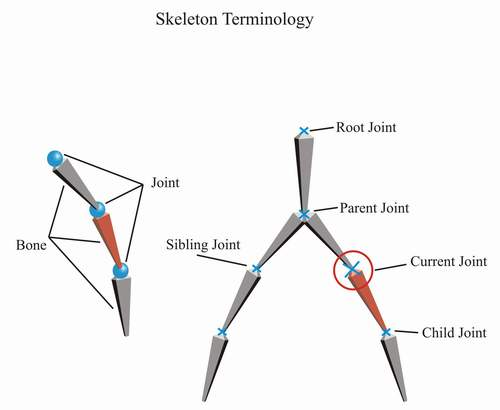
\includegraphics[width=0.8\columnwidth]{game/SkeletonTerminology.jpg}
		\caption[Sintesi della terminologia usata nelle animazioni scheletrali]{Sintesi della terminologia usata nelle animazioni scheletrali\footnotemark{} }
		\label{fig:SkeletonTerminology}
	\end{figure}
	\footnotetext{Tratto da \fullcite{site:skeleton-terminoligy}}
	
	Si procede quindi ad animare\footnote{Si consiglia al lettore appassionato \fullcite[chp.~24, 25]{inbook:directx-book} in cui è presente una breve introduzione alla matematica dei quaternioni, l'animazione scheletrale e lo skinning.} lo scheletro di animazione tramite la fisica o con delle pose fisse precalcolate dagli artisti, oppure con il blend tree calcolato tramite il middleware Emotion Fx.\\
	
	Il passo successivo è modificare la mesh dell'oggetto per rispecchiare l'animazione dello skeleton, questa procedura è detta Skinning. Un modo semplice per effettuarla è assegnare ad ogni vertice della mesh un massimo di 4 bone che potranno influenzarne la posizione. Si procede quindi (solitamente su GPU durante la fase di Vertex Shader) a calcolare un'interpolazione sulla trasformazione della posizione del vertice effettuando una media pesata fra i bone assegnati. La trasformazione risultante viene quindi applicata alla posizione originale del vertice.\\
	
	L'analisi del codice di gioco ha evidenziato la presenza di una precedente implementazione del disegno dello skeleton dei soli rider durante la corsa. Questa implementazione permetteva l'attivazione e la disattivazione della funzionalità di disegno attraverso una \texttt{define}.\\

	La prima modifica è stata l'esposizione nel Beholder di una variabile di membro di quella classe che permettesse di attivare/disattivare il disegno di debug a run-time.\\
	
	\begin{figure}[h!] 
		\centering 
		\hspace*{-0.05\columnwidth}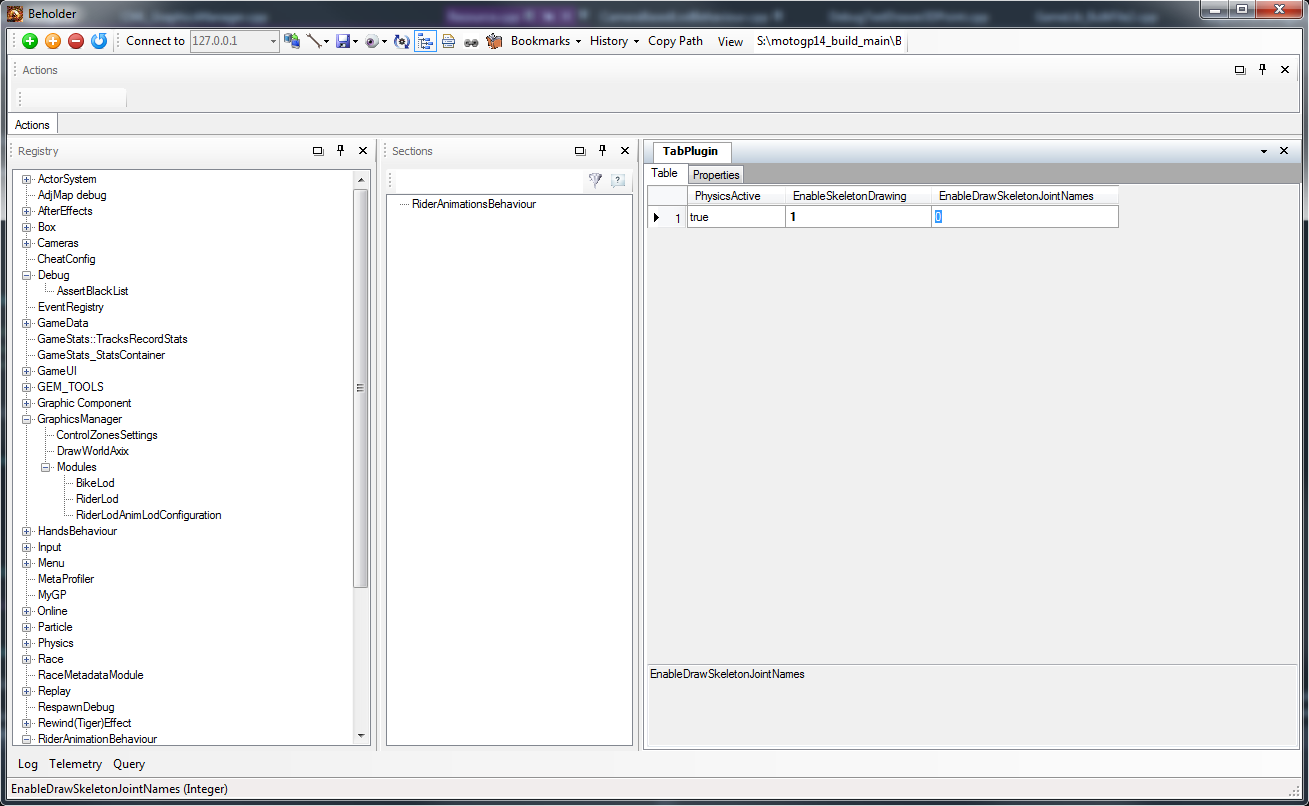
\includegraphics[width=1.1\columnwidth]{game/BeholderActivateRiderSkeleton.png} 
		\caption{Screenshot del Beholder in cui è possibile visualizzare dove è permesso attivare e disattivare il disegno dello skeleton del rider}
	\end{figure}
	
	Successivamente si è proceduto ad affinare e ottimizzare l'algoritmo di disegno, estrapolandolo e portandolo in una classe specializzata nel solo disegno di uno skeleton: \texttt{SkeletonDebugDrawer}.\\
	
	Di seguito è presente il codice della classe \texttt{SkeletonDebugDrawer}.
	
	\lstinputlisting[style=maurizio-code, caption=SkeletonDebugDrawer.h, label={code:SkeletonDebugDrawer-h}]{code/SkeletonDebugDrawer.h}
	
	\lstinputlisting[style=maurizio-code, caption=SkeletonDebugDrawer.cpp, label={code:SkeletonDebugDrawer-cpp}]{code/SkeletonDebugDrawer.cpp}
	~\\
	La rappresentazione interna dello scheletro organizzata come spiegato prima, permette quindi di utilizzare lo scheletro efficientemente minimizzando le moltiplicazioni tra matrici. L'algoritmo di disegno procede quindi ricorsivamente, con un approccio top-down, a calcolare l'effettiva posizione del joint corrente applicando la trasformazione del padre. In questo modo si evitano la ripetizione della stessa operazione che sarebbe emersa in un approccio bottom-up.\\
	
	\begin{figure}[h!] 
		\centering 
		\hspace*{-0.05\columnwidth}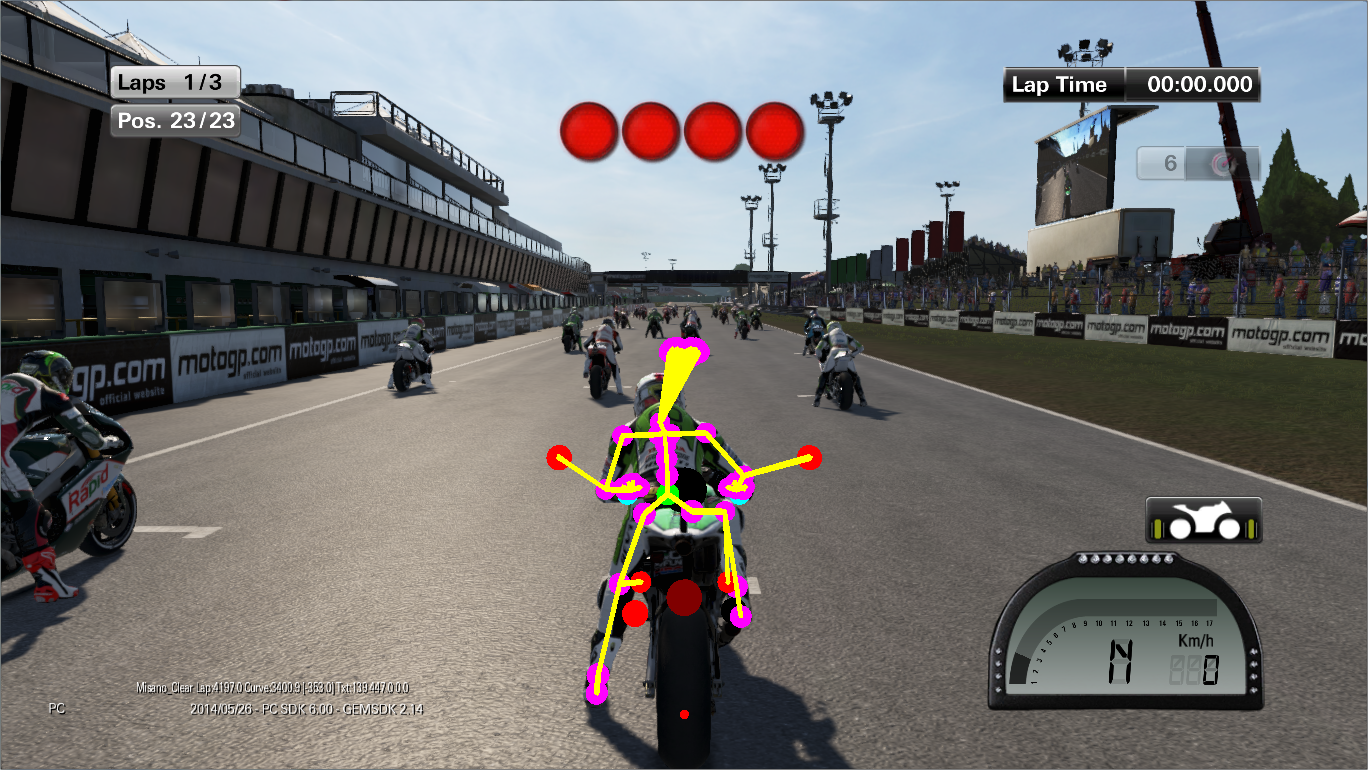
\includegraphics[width=1.1\columnwidth]{game/skeletonRider1.png} 
		\caption{Screenshot n. 1 del disegno dello skeleton del rider}
	\end{figure}
	
	\begin{figure}[h!] 
		\centering 
		\hspace*{-0.05\columnwidth}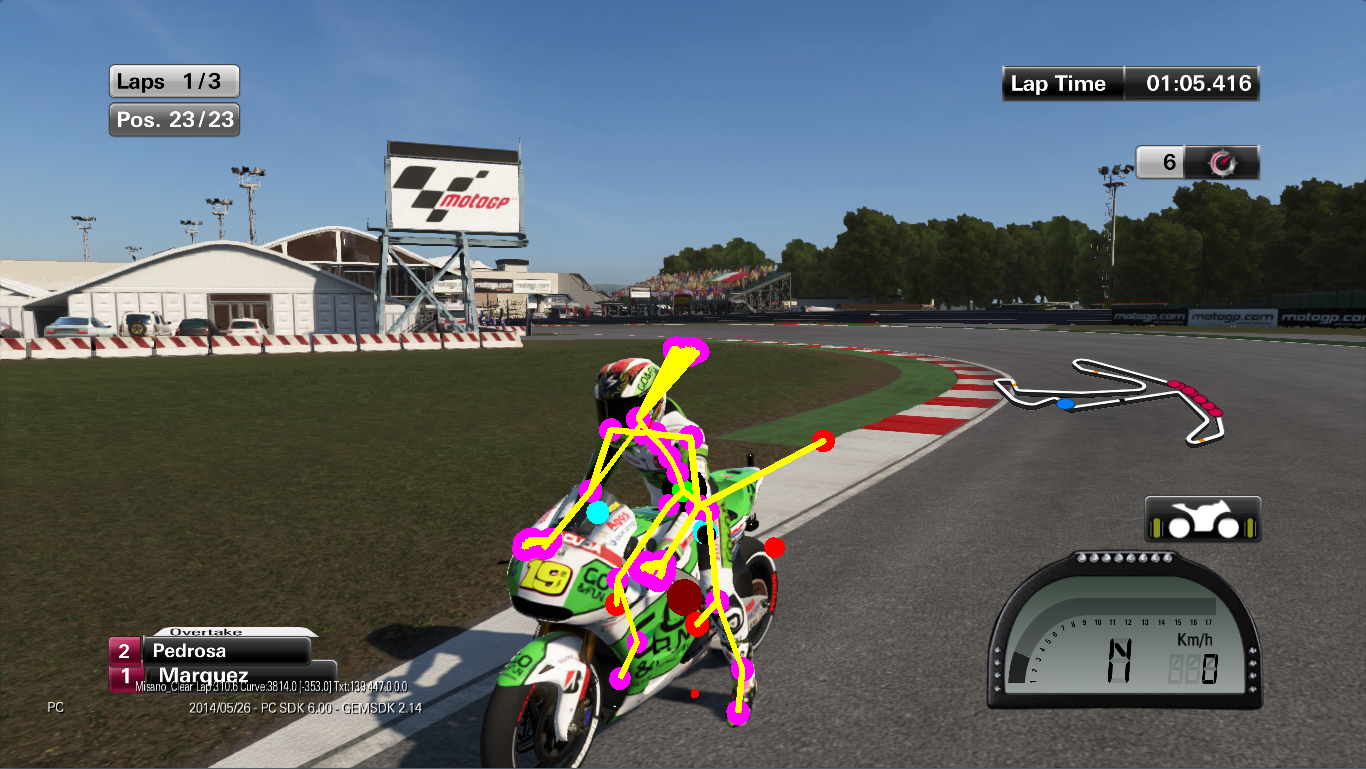
\includegraphics[width=1.1\columnwidth]{game/skeletonRider2.png} 
		\caption{Screenshot n. 2 del disegno dello skeleton del rider}
	\end{figure}
	
	Un altro obbiettivo era quello di disegnare lo scheletro di animazione non solo del rider corrente ma, di un qualsiasi oggetto animato.\\
	
	Per soddisfare questo obbiettivo si è ricorsi al \texttt{ResourcesManagerDebug}. Esso contenendo tutti gli oggetti era il posto corretto da cui partire. Per ogni \texttt{CObject3d} si è proceduto a valutare se era un oggetto animato e nel caso, permettere all'utente tramite Beholder di lanciare il disegno dello scheletro.\\
	
	Per capire se un oggetto è animato si è ricorsi ad un dynamic\_cast da \texttt{CObject3d} a \texttt{CAnimated3dModel}, sottoclasse che rappresenta gli oggetti 3d anche animati. Nel codice il dynamic\_cast è stato poi sostituito con un più veloce confronto tra ClassID.\\
	
	Per gli oggetti animati è stato quindi inserito nel Beholder la possibilità di lanciarne il disegno dello scheletro. Essendo il disegno dello scheletro un'azione da compiere ad ogni frame, vista la sua continua modifica, si è proceduto a creare la classe \texttt{SkeletonDebugDrawerManager}. Essa permette di aggiungere un oggetto il cui scheletro verrà disegnato ogni frame. Permette inoltre di mettere in pausa il disegno oppure di fermare definitivamente il disegno.\\
	
	Come già accennato tutte queste funzionalità sono disponibili da Beholder, in particolare per ogni oggetto visualizzato nel Beholder tramite il \texttt{ResourcesManagerDebug} è presente una proprietà che indica (true o false) se l'oggetto è animato, e quindi è possibile disegnarne lo scheletro.\\
	
	In figura \ref{fig:resource-manager-tree-view} è visibile sulla destra le proprietà di un oggetto 3D, tra le quali \texttt{isAnimated}. In alto a sinistra invece ci sono le azioni disponibili, tra le quali il disegno dello scheletro. Azione che verrà davvero eseguita solo se l'oggetto è animato.\\
	
	Di seguito è presente il codice della classe \texttt{SkeletonDebugDrawerManager}.
	
	\begin{figure}[h!] 
		\centering 
		\hspace*{-0.05\columnwidth}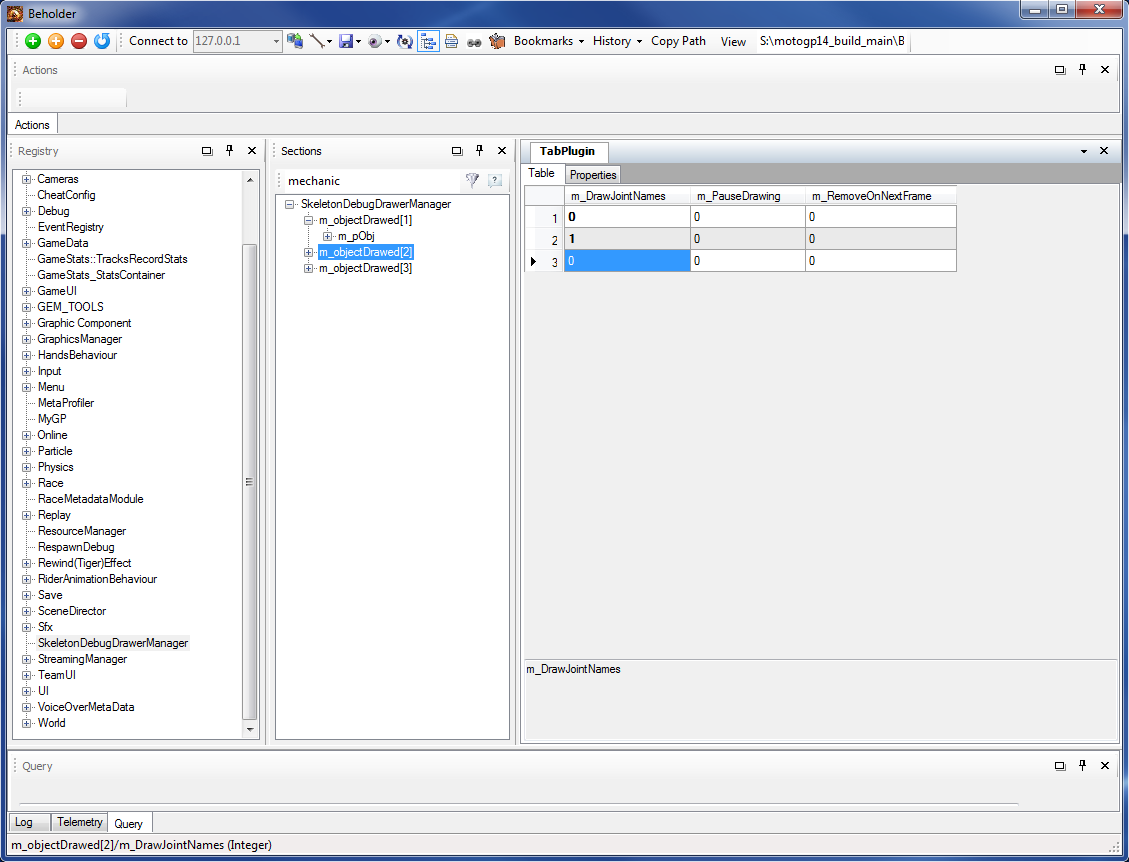
\includegraphics[width=1.1\columnwidth]{game/SkeletonDebugDrawerManagerinBeholder.png} 
		\caption{Screenshot del Beholder in cui è visibile lo \texttt{SkeletonDebugDrawerManager}}
	\end{figure}
	
	\begin{figure}[b!] 
		\centering
		\hspace*{-0.05\columnwidth}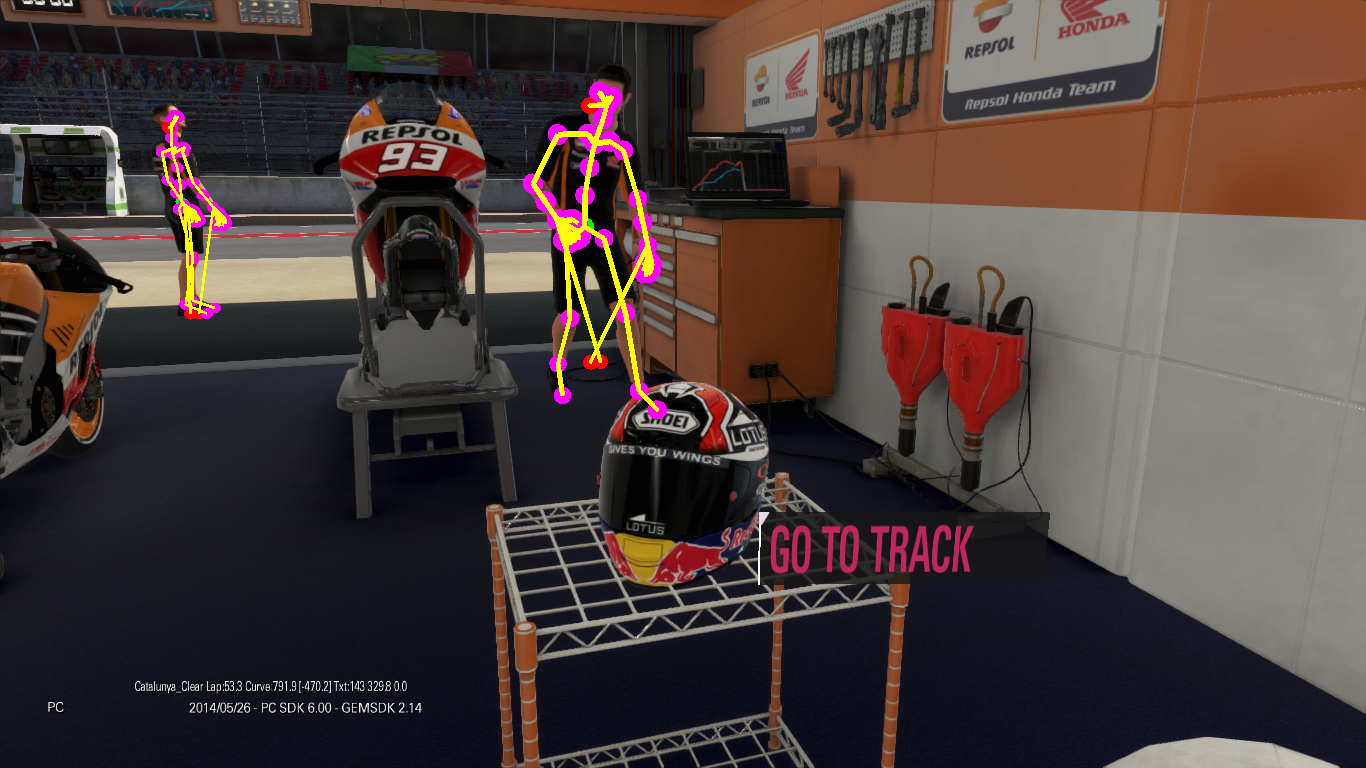
\includegraphics[width=1.1\columnwidth]{game/mechanicSkeleton.png} 
		\caption{Screenshot di MotoGP 14 in cui è stato attivato il disegno degli scheletri di animazione di 2 meccanici}
	\end{figure}
	
	\lstinputlisting[style=maurizio-code, caption=SkeletonDebugDrawerManager.h, label={code:SkeletonDebugDrawerManager-h}]{code/SkeletonDebugDrawerManager.h}
	
	\lstinputlisting[style=maurizio-code, caption=SkeletonDebugDrawerManager.cpp, label={code:SkeletonDebugDrawerManager-cpp}]{code/SkeletonDebugDrawerManager.cpp}             % Product Design Freeze e SOP
% !TEX encoding = UTF-8
% !TEX TS-program = pdflatex
% !TEX root = ../tesi.tex
% !TEX spellcheck = it-IT

%**************************************************************
\chapter{Conclusioni}
\label{cap:conclusioni}
%**************************************************************

In questo capitolo verranno presentate le riflessioni scaturite dall'analisi effettuata a posteriori dell'esperienza di stage. Verranno analizzati gli obbiettivi raggiunti e l'esperienza acquisita durante il lavoro, concludendo con una valutazione di come la preparazione accademica si interfacci con il mondo del lavoro.

%**************************************************************
\section{Raggiungimento degli obbiettivi}

Lo studente ha raggiunto tutti gli obbiettivi pianificati ad inizio stage, con soddisfazione dell'azienda e del tutor esterno. Questa ha infatti proposto allo studente altri sei mesi di collaborazione per continuare il percorso iniziato e la formazione on-the-job.\\

I tool sviluppati durante la prima parte dello stage sono infatti stati apprezzati e verranno presto inseriti nel modus operandi aziendale. In essi lo studente ha soddisfatto tutti i requisiti posti in fase di analisi degli stessi, seppur sforando di 4 giorni lavorativi sul tempo pianificato per la conclusione definitiva di XML Editor. Tempo recuperato poi durante lo svolgimento della seconda parte.\\

Di seguito viene riportata una tabella ed un grafico contenenti il resoconto della suddivisione delle ore per macro attività ed il confronto fra le ore preventivate e quelle a consuntivo. Le ore riportate di seguito sono comprensive del tempo dedicato alla stesura della documentazione.

\begin{center}
	\begin{longtable}{p{3.2cm}!{\color{white}\vrule width 0.5mm}c!{\color{white}\vrule width 0.5mm}c!{\color{white}\vrule width 0.5mm}c!{\color{white}\vrule width 0.5mm}}
		\rowcolor{headcolor}\textcolor{white}{\textbf{Attività}}&\textcolor{white}{\textbf{Ore a preventivo}}&\textcolor{white}{\textbf{Ore a consuntivo}} & \textcolor{white}{\textbf{Variazione}} \\
		
		\rowcolor{row1} Analisi & 130 & 110 & -20\\
		\rowcolor{row2} Progettazione & 45 & 65 & +20\\
		\rowcolor{row1} Codifica & 85 & 90 & +5\\
		\rowcolor{row2} Verifica & 60 & 55 & -5\\
		\rowcolor{row1} \textbf{Totale} & \textbf{320} & \textbf{320} & \textbf{0}\\
		\caption{Riepilogo ore a preventivo e consuntivo}
		\label{tab:istoBilancio}
	\end{longtable}
\end{center}

\begin{figure}[h!] 
	\centering 
	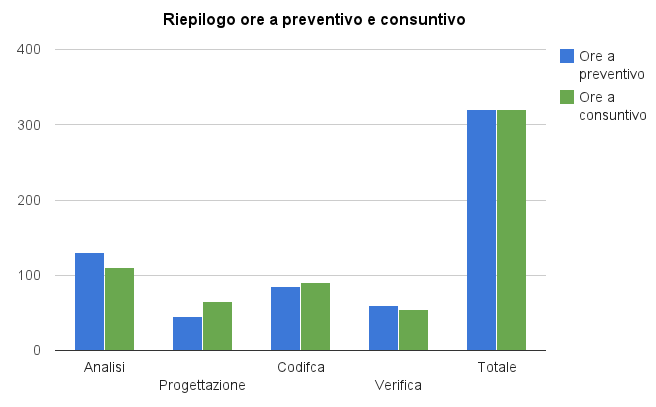
\includegraphics[width=1\columnwidth]{bilancio.png} 
	\caption{Istogramma del riepilogo ore a preventivo e consuntivo}
	\label{fig:istoBilancio}
\end{figure}

\newpage

Come visibile in tabella \ref{tab:istoBilancio} ed in figura \ref{fig:istoBilancio} si nota che l'attività di analisi e formazione ha occupato 20 ore meno del previsto, le quali sono state quasi tutte reinvestite in progettazione, spiegabile dalla complessità del sistema con il quale lo studente ha interagito.\\

La codifica invece ha portato via poco in più di ciò preventivato e, vista l'impossibilità di aumentare il budget ore complessivo, si è stati costretti a tagliare sulla verifica.

%**************************************************************
\section{Conoscenze acquisite e valutazione della preparazione accademica}

Lo studente ha approfondito la sua conoscenza delle librerie Qt\textsuperscript{\textregistered}, soprattutto ha potuto maturare esperienza nella progettazione di un'architettura che si adattasse al meglio con il framework in questione e che al contempo risultasse facilmente comprensibile ed estendibile. Egli ha potuto inoltre mettere in pratica le conoscenze di usabilità nel progettare la user interface dei tool, acquisite nei corsi di Tecnologie Web.\\

Lo stagista ha inoltre potuto approfondire le proprie conoscenze nella grafica 3D, sopratutto nell'ambito delle animazioni scheletrali. C'è da dire, sotto questo aspetto, che le competenze necessarie per svolgere gli obbiettivi della seconda parte sono state acquisite dallo studente in maniera autonoma durante tutto il percorso di studi, utilizzando come basi per comprendere le nuove nozioni ciò studiato durante il percorso accademico.\\

Tranne le conoscenze di grafica 3D bisogna affermare che la preparazione fornita durante il percorso di studi è stata adeguata alle necessità aziendali. Durante lo sviluppo si è potuto constatare che il metodo di lavoro acquisito si adattava bene a quello aziendale.\\

Si è constatato inoltre la necessità di autonomia nella ricerca e nell'approfondimento di particolare tematiche di cui lo studente non era a conoscenza con gli strumenti a disposizione (internet e manuali).\\

Tutto il codice prodotto, sopratutto quello dei tool, è stato documentato nel migliore dei modi per poter permettere a chiunque di comprenderlo ed evolverlo in completa autonomia.\\

È convinzione dello studente che, al di là degli aspetti teorici e pratici di qualunque tecnologia, un informatico maturo che abbia compreso gli aspetti fondamentali dell'informatica insegnati in questo corso di studio, potrà durante la sua intera carriera acquisire senza troppi problemi tutte le tecnologie di cui avrà bisogno.

%**************************************************************
\section{Valutazione personale}

Lo studente ritiene che lo stage sia stata un'esperienza decisamente positiva, oltre agli obbiettivi raggiunti, l'ambiente in cui è stato inserito si è dimostrato positivo e amichevole. La positività che lo stagista ha sempre dimostrato è stata ricambiata dai colleghi e dalla direzione che ha confermato la collaborazione. Altro motivo di crescita è derivato dal trasferimento a Milano, sede di Milestone S.r.l., per lo svolgimento del tirocinio, che ha permesso allo studente di crescere e maturare anche da questo punto di vista.\\

Per tutti questi motivi si afferma la buona riuscita del periodo di stage.
             % Conclusioni
\appendix                               
% !TEX encoding = UTF-8
% !TEX TS-program = pdflatex
% !TEX root = ../tesi.tex
% !TEX spellcheck = it-IT

%**************************************************************
\chapter{Appendice A}
%**************************************************************

\epigraph{Citazione}{Autore della citazione}



             % Appendice A

%**************************************************************
% Materiale finale
%**************************************************************
\backmatter
\printglossaries
% !TEX encoding = UTF-8
% !TEX TS-program = pdflatex
% !TEX root = ../tesi.tex
% !TEX spellcheck = it-IT

%**************************************************************
% Bibliografia
%**************************************************************

\cleardoublepage
\chapter{Bibliografia}

\nocite{*}
%\addtocategory{opere}{site:milestone}
\addtocategory{web}{site:milestone}

\bibbycategory % equivale a dare un \printbibliography per ogni categoria

\end{document}
